% -----------------------------------------------------------------------------
%       Centro Federal de Educação Tecnológica de Minas Gerais - CEFET-MG
%
%   Modelo de trabalho acadêmico monográfico de acordo com as normas da ABNT
%   (Tese de Doutorado, Dissertação de Mestrado ou Projeto de Qualificação)
%
%     Projeto hospedado em: https://github.com/cfgnunes/latex-cefetmg
%
%    Autores: Cristiano Fraga G. Nunes <cfgnunes@gmail.com>
%             Henrique E. Borges <henrique@lsi.cefetmg.br>
%             Denise de Souza <densouza@gmail.com>
%             Lauro César <https://code.google.com/p/abntex2/>
%
% -----------------------------------------------------------------------------

\documentclass[%
%    twoside,                    % Impressão em frente (anverso) e verso
    oneside,                    % Impressão apenas no anverso
]{cefetmg}

\usepackage[%
    num,
%    overcite,
    abnt-emphasize=bf,
    bibjustif,
    recuo=0cm,
    abnt-doi=expand,            % Expande um endereço iniciado com doi: para http://dx.doi.org/
    abnt-url-package=url,       % Utiliza o pacote url
    abnt-refinfo=yes,           % Utiliza o estilo bibliográfico abnt-refinfo
    abnt-etal-cite=3,
    abnt-etal-list=3,
    abnt-thesis-year=final
]{abntex2cite}                  % Configura as citações bibliográficas conforme a norma ABNT

% -----------------------------------------------------------------------------
% Pacotes utilizados
% -----------------------------------------------------------------------------
\usepackage[utf8]{inputenc}                                 % Codificação do documento
\usepackage[T1]{fontenc}                                    % Seleção de código de fonte
\usepackage{booktabs}                                       % Réguas horizontais em tabelas
\usepackage{color, colortbl}                                % Controle das cores
\usepackage{float}                                          % Necessário para tabelas/figuras em ambiente multi-colunas
\usepackage{graphicx}                                       % Inclusão de gráficos e figuras
\usepackage{icomma}                                         % Uso de vírgulas em expressões matemáticas
\usepackage{indentfirst}                                    % Indenta o primeiro parágrafo de cada seção
\usepackage{microtype}                                      % Melhora a justificação do documento
\usepackage{multirow, array}                                % Permite tabelas com múltiplas linhas e colunas
\usepackage{subeqnarray}                                    % Permite subnumeração de equações
\usepackage{verbatim}                                       % Permite apresentar texto tal como escrito no documento, ainda que sejam comandos Latex
\usepackage{amsfonts, amssymb, amsmath, wasysym, txfonts}   % Fontes e símbolos matemáticos
\usepackage[algoruled, english]{algorithm2e}                % Permite escrever algoritmos em inglês
\usepackage[scaled]{helvet}                                 % Usa a fonte Helvetica
%\usepackage{times}                                         % Usa a fonte Times
%\usepackage{palatino}                                      % Usa a fonte Palatino
%\usepackage{lmodern}                                       % Usa a fonte Latin Modern
%\usepackage[bottom]{footmisc}                              % Mantém as notas de rodapé sempre na mesma posição
%\usepackage{ae, aecompl}                                   % Fontes de alta qualidade
%\usepackage{latexsym}                                      % Símbolos matemáticos
%\usepackage{lscape}                                        % Permite páginas em modo "paisagem"
%\usepackage{picinpar}                                      % Dispor imagens em parágrafos
%\usepackage{scalefnt}                                      % Permite redimensionar tamanho da fonte
%\usepackage{subfig}                                        % Posicionamento de figuras
%\usepackage{upgreek}                                       % Fonte letras gregas
\usepackage{subcaption}                                     % Permite a utilização de sublegendas em finguras compostas
\usepackage{empheq}                                         % Permite a utilização de subequações
\usepackage{tikz}                                           % Criação e manipulação de figuras
\usepackage{tikzscale}                                      % Inclui as figuras feitas no TIKZ
\usepackage{pdfpages}                                       % Permite a inclusão de arquivos no texto

% Redefine o estilo de citação para o uso dos colchetes
\citebrackets[]

% Redefine a fonte para uma fonte similar a Arial (fonte Helvetica)
\renewcommand*\familydefault{\sfdefault}

% Redefine a cor dos números dos algoritmos para preto
% \SetNlSty{bfseries}{\color{black}}{}

% -----------------------------------------------------------------------------
% Configurações de aparência do PDF final
% -----------------------------------------------------------------------------
\makeatletter
\hypersetup{%
    english,
    colorlinks=true,            % true: "links" coloridos; false: "links" em caixas de texto
    linkcolor=black,            % Define cor dos "links" internos
    citecolor=black,            % Define cor dos "links" para as referências bibliográficas
    filecolor=black,            % Define cor dos "links" para arquivos
    urlcolor=black,             % Define a cor dos "hiperlinks"
    breaklinks=true,
    pdftitle={\@title},
    pdfauthor={\@author},
    pdfkeywords={Granular Materials, DEM, CFD, BNE}
}
\makeatother

% Altera o aspecto da cor azul
\definecolor{blue}{RGB}{41,5,195}

% Redefinição de labels
\renewcommand{\algorithmautorefname}{Algorithm}
\def\equationautorefname~#1\null{Equation~(#1)\null}

% Cria o índice remissivo
\makeindex

% Hifenização de palavras que não estão no dicionário
\hyphenation{%
    qua-dros-cha-ve
}

% -----------------------------------------------------------------------------
% Inclui os arquivos do trabalho acadêmico
% -----------------------------------------------------------------------------

% Insere e constrói alguns elementos pré-textuais para gerar capa, folha de rosto e folha de aprovação
% -----------------------------------------------------------------------------
% Capa
% -----------------------------------------------------------------------------

% -----------------------------------------------------------------------------
% ATENÇÃO:
% Caso algum campo não se aplique ao seu documento - por exemplo, em seu trabalho
% não houve coorientador - não comente o campo, apenas deixe vazio, assim: \campo{}
% -----------------------------------------------------------------------------

% -----------------------------------------------------------------------------
% Dados do trabalho acadêmico
% -----------------------------------------------------------------------------

\titulo{Numerical simulation of granular materials}
%\title{Title in English}
\subtitulo{Brazil nut effect and sediment transport}
\autor{Gustavo Henrique Borges Martins}
\local{Belo Horizonte}
\data{2021 August} % Normalmente se usa apenas mês e ano

% -----------------------------------------------------------------------------
% Natureza do trabalho acadêmico
% Use apenas uma das opções: Tese (p/ Doutorado), Dissertação (p/ Mestrado) ou
% Projeto de Qualificação (p/ Mestrado ou Doutorado), Trabalho de Conclusão de
% Curso (Graduação)
% -----------------------------------------------------------------------------

\projeto{Thesis}

% -----------------------------------------------------------------------------
% Título acadêmico
% Use apenas uma das opções:
% - Se a natureza for Tese, coloque Doutor
% - Se a natureza for Dissertação, coloque Mestre
% - Se a natureza for Projeto de Qualificação, coloque Mestre ou Doutor conforme o caso
% - Se a natureza for Trabalho de Conclusão de Curso, coloque Bacharel
% -----------------------------------------------------------------------------

\tituloAcademico{Doctor of Philosophy}

% -----------------------------------------------------------------------------
% Área de concentração e linha de pesquisa
% OBS: indique o nome da área de concentração e da linha de pesquisa do Programa de Pós-graduação
% nas quais este trabalho se insere
% Se a natureza for Trabalho de Conclusão de Curso, deixe ambos os campos vazios
% -----------------------------------------------------------------------------

\areaconcentracao{Mathematical and Computational Modeling}
\linhapesquisa{Applied Mathematical Methods}

% -----------------------------------------------------------------------------
% Dados da instituição
% OBS: a logomarca da instituição deve ser colocada na mesma pasta que foi colocada o documento
% principal com o nome de "logoInstituicao". O formato pode ser: pdf, jpf, eps
% Se a natureza for Trabalho de Conclusão de Curso, coloque em "programa' o nome do curso de graduação
% -----------------------------------------------------------------------------

\instituicao{Centro Federal de Educação Tecnológica de Minas Gerais}
\programa{Programa de Pós-graduação em Modelagem Matemática e Computacional}
\logoinstituicao{0.2}{./04-figuras/logo-instituicao.pdf} % \logoinstituicao{<escala>}{<nome do arquivo>}

% -----------------------------------------------------------------------------
% Dados do(s) orientador(es)
% -----------------------------------------------------------------------------

\orientador[Advisor:]{Allbens Atman Picardi Faria}
%\orientador[Orientadora:]{Nome da orientadora}
\instOrientador{CEFET-MG}

\coorientador[Co-Advisor:]{Philippe Claudin}
%\coorientador[Coorientadora:]{Nome da coorientadora}
\instCoorientador{ESPCI - France}

% -----------------------------------------------------------------------------
% Folha de Rosto
% -----------------------------------------------------------------------------

% Trabalho de Conclusão de Curso
%\preambulo{{\imprimirprojeto} apresentado ao Curso de Engenharia de Computação do Centro Federal de Educação Tecnológica de Minas Gerais, como requisito parcial para a obtenção do título de {\imprimirtituloAcademico} em Engenharia de Computação.}

% Projeto de qualificação de Mestrado ou Doutorado
%\preambulo{{\imprimirprojeto} apresentado ao Programa de \mbox{Pós-graduação} em Modelagem Matemática e Computacional do Centro Federal de Educação Tecnológica de Minas Gerais, como requisito parcial para a obtenção do título de {\imprimirtituloAcademico} em Modelagem Matemática e Computacional.}

% Dissertação de Mestrado
%\preambulo{{\imprimirprojeto} apresentada ao Programa de \mbox{Pós-graduação} em Modelagem Matemática e Computacional do Centro Federal de Educação Tecnológica de Minas Gerais, como requisito parcial para a obtenção do título de {\imprimirtituloAcademico} em Modelagem Matemática e Computacional.}

% Tese de Doutorado
\preambulo{{\imprimirprojeto} presented to the \mbox{Graduate Program} in Mathematical and Computational Modeling at Centro Federal de Educação Tecnológica de Minas Gerais, as partial requirement to obtain the degree of {\imprimirtituloAcademico} in Mathematical and Computer Modeling.}
%\preambulo{{\imprimirprojeto} apresentada ao Programa de \mbox{Pós-graduação} em Modelagem Matemática e Computacional do Centro Federal de Educação Tecnológica de Minas Gerais, como requisito parcial para a obtenção do título de {\imprimirtituloAcademico} em Modelagem Matemática e Computacional.}

% -----------------------------------------------------------------------------
% Edite este arquivo comentando as linhas que não se aplicam ao tipo de documento acadêmico pretendido.
% -----------------------------------------------------------------------------

% -----------------------------------------------------------------------------
% Folha de Aprovação
% -----------------------------------------------------------------------------

\textopadraofolhadeaprovacao{This sheet should be replaced by the scanned copy of the approval sheet provided.}

% -----------------------------------------------------------------------------
% Este documento foi mantido apenas para preservar a paginação do trabalho
% acadêmico final, após a inserção da folha de aprovação fornecida
% -----------------------------------------------------------------------------


\begin{document}

% Insere os elementos pré-textuais
\pretextual
\imprimircapa                                               % Comando para imprimir Capa
\imprimirfolhaderosto{}                                     % Comando para imprimir Folha de rosto
\imprimirfolhadeaprovacao{}                                 % Comando para imprimir Folha de aprovação
%% -----------------------------------------------------------------------------
% Dedicatória
% -----------------------------------------------------------------------------

\begin{dedicatoria}

I dedicate this thesis to all teachers that went in my life, 'cause without them, for sure, I wouldn't know that my profession is to be an eternal questioner...

\textit{Dedico este texto a todos os meus professores, pois sem eles, com certeza, não saberia que a minha profissão é ser um eterno aprendiz...}

\textit{Je dédie cette thèse à tous les enseignants et professeurs qui sont allés dans ma vie, car sans eux, surement, je ne saurais pas que ma profession est devenir un éternel questionneur ... Merci a vous !}

\end{dedicatoria}
           % Dedicatória
%% -----------------------------------------------------------------------------
% Agradecimentos
% -----------------------------------------------------------------------------

\begin{agradecimentos}[Acknowledgements]

First of all, I am greatfull to the creator of the universe, that gaves us inteligence and mysteries, which through science and philosophy will be unveiled.

To my family, I am thankful that they always given me all the encouragement and support necessary to carry out all my human and academic training. To my beloved wife, that supported me in all ways to keep searching and understanding what are the misteries of nature. To my father, I thank who always encouraged me to study scientific. To my mother, I thank, taste and fulfillment for teaching. To my brother I thank all the practice of patience and perseverance, in addition to keeping me in the realization of good practices and the usefulness of our work.

To my friend and adviser Allbens Atman, I thank the time and the efforts to teach me the path of the research and to all lessons inside and outside class, that I take with me.

To my friend and co-adviser Philippe Claudin, I thank for accepting me as his student, besides all disponibility and pacience that leads to this research.

I thank to the support given from the Graduate Program in Mathematical and Computing Modelling - PPGMMC at \textit{Centro Federal de Educação Tecnológica de Minas Gerais} - CEFET-MG, and from the laboratory \textit{Physique et Mécanique des Milieux Hétérogènes} - PMMH at \textit{École Supérieure de Physique et de Chimie Industrielles de la ville de Paris} - ESPCI.

I am also thankful to all my teachers and professors, once without them, I would certainly not be here.

To my friends, I thank their compreension, whom give me support in this project.

And specially, I am greatful to every brazilian citzen, that allow me to do this research in this public institution payed with taxes. I am also greatful to the finacial support given by \textit{Conselho Nacional de Pesquisa} - CNPq grant 88881.187077/2018-01, \textit{Coordenação de aperfeiçoamento de Pessoal de Nível Superior} - CAPES, \textit{Fundação de Amparo à Pesquisa do Estado de Minas Gerais} - FAPEMIG, PPGMMC, CEFET-MG, PMMH, \textit{Centre National de la Recherce Scientifique} - CNRS, and \textit{Fundação CEFETMINAS}.

%É obrigatório o agradecimento às instituições de fomento à pesquisa que financiaram total ou parcialmente o trabalho, inclusive no que diz respeito à concessão de bolsas.

\end{agradecimentos}

\begin{agradecimentos}[Agradecimentos]

Agradeço primeiramente ao grande criador de todo o universo, que nos deu inteligência e os mistérios, que pelas ciências e filosofia os serão desvendados.

À minha família, que sempre deu todo o incentivo e suporte necessários para realizar toda a minha formação humana e acadêmica. À minha grande companheira que sempre me deu apoio e incentivo, direto e indireto, a sempre continuar desvendando os mistérios naturais. Ao meu pai que sempre me incentivou o estudo científico. A minha mãe o gosto e a realização pela docência. Ao meu irmão toda a prática de paciência e perseverança, além de me manter na realização das boas práticas e da utilidade de nossos trabalhos.

Ao meu amigo e orientador Allbens Atman, por todo o tempo e esforço em ensinar os caminhos de como fazer pesquisa e por todas as lições dentro e fora da sala de aula que levo comigo.

Ao meu amigo e co-orientador Philippe Claudin, por ter me aceitado como seu aluno, além de toda a disponibilidade e paciência para que pudessemos chegar neste estágio da pesquisa.

Ao Centro Federal de Educação Tecnológico de Minas Gerais - CEFET-MG, ao Programa de Pós-Graduação em Modelagem Matemática e Computacional - PPGMMC e ao laboratório de \textit{Physique et Mécanique des Milieux Hétérogènes} - PMMH da \textit{École Supérieure de Physique et de Chimie Industrielles de la ville de Paris} - ESPCI que disponibilizaram seus recursos, pessoal e apoio nesta pesquisa.

À todos os meus professores, que certamente contribuíram para a minha chegada até este ponto.

Aos meus amigos e colegas que sempre compreenderam as ausências, e que me deram a ajuda e o suporte para continuar trabalhando neste projeto, sejam como ouvidos para os desabafos, sejam para renovar as ideias da pesquisa.


%É obrigatório o agradecimento às instituições de fomento à pesquisa que financiaram total ou parcialmente o trabalho, inclusive no que diz respeito à concessão de bolsas.

À cada cidadão brasileiro, que me permitiu pesquisar em uma escola paga com os impostos do povo, através de suas agências de fomento à educação e à pesquisa. Ao Conselho Nacional de Pesquisa - CNPq, especialmente na chamada de número 88881.187077/2018-01, à Coordenação de Aperfeiçoamento de Pessoal de Nível Superior - CAPES, à Fundação de Amparo à Pesquisa do Estado de Minas Gerais - FAPEMIG, ao CEFET-MG, ao PMMH e à ESPCI, ao \textit{Centre National de la Recherche Scientifique} - CNRS e à Fundação CEFETMINAS pelo suporte financeiro neste projeto de pesquisa, que teve início desde minha primeira iniciação científica em 2008.

\end{agradecimentos}
        % Agradecimentos
%% -----------------------------------------------------------------------------
% Epígrafe
% -----------------------------------------------------------------------------

\begin{epigrafe}

%\textit{“Saber que sabemos o que sabemos, e saber que não sabemos o que não sabemos, esta é a verdadeira sabedoria.”}
%(Nicolau Copérnico)

%\textit{“São grandes as vantagens industriais derivadas do princípio econômico da divisão do trabalho, porém, por causa disso, privou-se o trabalho do homem de alma e de vida.”}
%(Johannes Kepler)

\textit{“All truths are easy to understand once they are discovered; the point is discover them.”}

\textit{“Todas as verdades são fáceis de perceber depois de terem sido descobertas; o problema é descobri-las.”}

\textit{"Il est facile comprendre toutes les vérités une fois qu'elles sont découvertes ; le point est de les découvrir."}

(Galileu Galilei)

%\textit{“A gravidade explica os movimentos dos planetas, mas não pode explicar quem colocou os planetas em movimento. Deus governa todas as coisas e sabe tudo que é ou que pode ser feito.”}
%(Isaac Newton)

%\textit{“Ninguém é tão sábio que não tenha algo pra aprender e nem tão tolo que não tenha algo pra ensinar.”}
%(Blaise Pascal)

%\textit{“Devemos admitir com humildade que, ao passo que os números são puramente produtos de nossas mentes, o espaço tem uma realidade fora de nossas mentes, de modo que não podemos descrever completamente suas propriedades a priori.”}
%(Carl Friedrich Gauss)

%\textit{“Leia Euler, leia Euler, ele é o mestre de todos nós.”}
%(Pierre Simon Laplace)

\end{epigrafe}

% -----------------------------------------------------------------------------
% Edite o texto acima para inserir uma epígrafe de sua preferência
% -----------------------------------------------------------------------------
              % Epígrafe
% -----------------------------------------------------------------------------
% Abstract
% -----------------------------------------------------------------------------

\begin{resumo}[Abstract]
    The simulation of granular materials is studied widely in many research centers around the world, and used in industries and engineering companies. For the understanding and quantification of granular materials a Discrete Element Method (DEM) simulates the behavior of granular materials.
    Many of the challenges to understanding the behavior of granular materials begin in the dry grain segregation phenomenon. Classically, we have the Brazil-Nut Effect (BNE) - which consists of confined granular material containing grains of different sizes and, when agitated, segregation occurs, with the larger grains rising from the mixture. For many years, it was believed that this segregation occurred due to the presence of walls that confine the material. In this thesis we show that in systems with periodic boundary conditions, BNE can also occur.
    We also studied sediment transport that occurs in the interaction between granules and fluids. To simulate the behavior of granular materials immersed in a fluid, we use a Computational Fluid Dynamics (CFD) technique. The solid sediments move in the velocity field transported by the fluid. Three dimensionless parameters are required to describe the transport behavior: the Reynolds number, which relates the inertial forces to the viscous forces, and consequently the fluid turbulence effects; the number of Shields, which is related to the drag forces and the inertial forces of the fluid; and finally, the density ratio between the solid and the fluid. It is possible to reproduce the different modes of transport only by changing such dimensionless parameters. In this thesis, we calculate the saturation time for the modes of transport.
%    Translation of the abstract into english, possibly adapting or slightly changing the text in order to adjust it to the grammar of Standard English.
%    Try to stay within the limit of: 500 word for a PhD Thesis;
%    250 words for a Master Dissertation;
%    200 words for a Qualifying Research Project.

    \textbf{Keywords}: Granular materials. Computer simulations. Discrete Element Method (DEM). Computational Fluid Dynamics (CFD). Brazil-Nut Effect. Sediment transport.
\end{resumo}

% -----------------------------------------------------------------------------
% O restante da formatação deve manter-se igual ao do resumo em português, i.e, um único parágrafo.
% -----------------------------------------------------------------------------
             % Resumo na língua vernácula
% -----------------------------------------------------------------------------
% Resumo
% -----------------------------------------------------------------------------

\begin{resumo}
    A simulação de materiais granulares é estudada nas academias de todo o mundo, também aplicada em indústrias e empresas de engenharia. Para o entendimento e quantificação das proprieadades dos materiais granulares, o Método de Elementos Discretos, ou \textit{Discrete Element Method} (DEM), é usado para simular o comportamento de materiais granulares.
    Muitos dos desafios de se compreender o comportamento de materiais granulares têm início no fenômeno de segregação de grãos secos. Classicamente, temos o efeito castanha do Pará - \textit{Brazil Nut Effect} (BNE) - que consiste em um material granular confinado contendo grãos de diferentes volumes e que, quando agitados, exibem segregação, sendo que os grãos maiores ascendem até a superfície. Por muitos anos, acreditou-se que esta segregação ocorria devido a presença de paredes que confinam o material. Nesta tese mostramos que em sistemas com condição periódica de contorno também pode ocorrer o BNE. Propomos que o BNE se comporta com efeito ressonate, e diferenciamos os sistemas com paredes do com condição periódica de contorno usando a função de grandes desvios - \textit{Large-Deviation function} (LDF).
    Estudamos também o transporte de sedimentos que ocorre na interação entre granulares e fluidos. Para simular o comportamento de materiais granulares imersos em um fluido, utilizamos uma técnica de Fluidodinâmica Computacional, ou \textit{Computational Fluid Dynamics} (CFD). Os sedimentos sólidos se movem em um campo de velocidades transportados pelo fluido. Três parâmetros adimensionais são necessários para descrever o comportamento do transporte: o número de Reynolds, que relaciona as forças inerciais com as forças viscosas, e consequentemente os efeitos de turbulência do fluido; o número de Shields, que está relacionado com a as forças de arraste e as forças inerciais do fluido; e finalmente, a razão de densidade entre o sólido e a fase fluida. É possível reproduzir os diferentes modos de transporte apenas mudando tais parâmetros adimensionais. Nesta tese, calculamos o tempo de saturação para o modo \textit{bedload} no regime viscoso, e também predizemos o tempo de saturação para este mode de transporte. Este estudo de transporte de sedimentos foi possível graças ao doutorado sanduíche realizado no PMMH-ESPCI com a bolsa CAPES No.88881.187077/2018-01.

    \textbf{Palavras Chaves}: Materiais granulares. Simulação computacional. Método de Elemento Discreto (DEM). Fluidodinâmica Computacional (CFD). Efeito castanha do Pará (BNE). Transporte de sedimentos.

%    Síntese do trabalho em texto cursivo contendo um único parágrafo.
%    Para uma Tese de Doutorado o resumo deve conter, no máximo, 500 palavras.
%    Para uma Dissertação de Mestrado o resumo deve conter, no máximo, 250 palavras.
%    Para um Projeto de Qualificação o resumo deve conter, no máximo, 200 palavras.
%    O resumo é a apresentação clara, concisa e seletiva do trabalho.
%    No resumo deve-se incluir, preferencialmente, nesta ordem:brevíssima introdução ao assunto do trabalho de pesquisa (incluindo motivação e justificativa para a realização deste trabalho), o que será feito no trabalho (objetivos), como ele será desenvolvido (metodologia), quais são os principais resultados obtidos ou esperados e a conclusão (compare os resultados com os da literatura e destaque as principais contribuições científicas do trabalho.

%    \textbf{Palavras-chave}: Modelo Latex. Trabalho acadêmico monográfico. Normas ABNT. Outra palavra.
\end{resumo}

% -----------------------------------------------------------------------------
% Escolha de 3 a 6 palavras ou termos que descrevam bem o seu trabalho. As palavras-chaves são utilizadas para indexação.
% A letra inicial de cada palavra deve estar em maiúsculas. As palavras-chave são separadas por ponto.
% -----------------------------------------------------------------------------
             % Resumo em língua inglesa
% -----------------------------------------------------------------------------
% Resumo
% -----------------------------------------------------------------------------

\begin{resumo}[Résumé]
    Des simulation de matériaux granulaires ont étudiée en centres de recherche de tout le monde, également elles ont appliquée dans les industries et des société d'ingénierie. Pour comprenez et qualifiez des propriétés des matériaux granulaire, la Méthode de Éléments Discrètes, ou \textit{Discrete Element Method} (DEM), est utilisée pour simuler des comportement des matériaux granulaires.
    De nombreux défis pour comprenez le comportement des matériaux granulaires commencement par le phénomène de ségrégation de grains secs. Classiquement, il y a l'effet noix du Brésil - \textit{Brazil Nut Effect} (BNE) - qui consiste en des matériaux granulaires confinés contenant grains de différents volumes et qui, lorsqu'ils son agités, présentent une ségrégation, le plus gros grains remontent jusqu'à la surface. Pendant de nombreuses années, on a cru que cette ségrégation était due à la présence de murs qui confinement le matériau. Dans cette thèse, nous montrons que dans le systèmes avec de condition aux limites périodiques, le BNE peut également se produire. Nous avons également proposé que le BNE présente un effet de résonance, et nous différencions les systèmes avec murs et de condition aux limites périodiques en utilisant la fonction de grande déviation.
    Nous avons également étudié le transport des sédiments qui se produit dans l'interaction entre le granules et les fluides. Pour simuler le comportement de matériaux granulaires immergés dans un fluide, nous utilisons une technique de Dynamique des Fluides Computationnelle, ou \textit{Computational Fluid Dynamics (CFD)}. Les sédiments solides se déplacent dans un champ de vitesses portées par le fluide. Trois paramètres adimensionnels sont nécessaires pour décrie le comportement de transport: le nombre de Reynolds, qui est lié aux forces d'inertie aux forces visqueuses, et par conséquent aux effets de la turbulence des fluides; le nombre de Shields, qui est lié aux forces de traînée et aux forces d'inertie du fluide; et enfin, le rapport de densité entre le solide et la phase fluide. Il est possible de reproduire les différents modes de transport simplement en modifiant ces paramètres adimensionnelles. Dans cette thèse, nous calculons et caractérisons le temps de saturation pour le modes de transport charrié en régime visquex, et nous prédisons également la longueur de saturation pour ce mode de transport. Ce transport sédimentaire a pu être étudié grâce à le stage de thèse fait au PMMH-ESPCI avec la bourse CAPES 88881.187077/2018-01.

    \textbf{Mots clés}: Matériaux granulaires. Simulation par ordinateur. Méthode des éléments discrets (DEM). Dynamique des fluides computationnelle (CFD). Effet de Noix du Brésil (BNE). Transporte de sédiments.

%    Síntese do trabalho em texto cursivo contendo um único parágrafo.
%    Para uma Tese de Doutorado o resumo deve conter, no máximo, 500 palavras.
%    Para uma Dissertação de Mestrado o resumo deve conter, no máximo, 250 palavras.
%    Para um Projeto de Qualificação o resumo deve conter, no máximo, 200 palavras.
%    O resumo é a apresentação clara, concisa e seletiva do trabalho.
%    No resumo deve-se incluir, preferencialmente, nesta ordem:brevíssima introdução ao assunto do trabalho de pesquisa (incluindo motivação e justificativa para a realização deste trabalho), o que será feito no trabalho (objetivos), como ele será desenvolvido (metodologia), quais são os principais resultados obtidos ou esperados e a conclusão (compare os resultados com os da literatura e destaque as principais contribuições científicas do trabalho.

%    \textbf{Palavras-chave}: Modelo Latex. Trabalho acadêmico monográfico. Normas ABNT. Outra palavra.
\end{resumo}

% -----------------------------------------------------------------------------
% Escolha de 3 a 6 palavras ou termos que descrevam bem o seu trabalho. As palavras-chaves são utilizadas para indexação.
% A letra inicial de cada palavra deve estar em maiúsculas. As palavras-chave são separadas por ponto.
% -----------------------------------------------------------------------------
             % Resumo em língua francesa
% -----------------------------------------------------------------------------
% Lista de Figuras
% -----------------------------------------------------------------------------

\pdfbookmark[0]{\listfigurename}{lof}
\listoffigures*
\cleardoublepage

% -----------------------------------------------------------------------------
% Este arquivo não necessita de ser editado. A lista é gerada automaticamente.
% -----------------------------------------------------------------------------
         % Lista de figuras
% -----------------------------------------------------------------------------
% Lista de Tabelas
% -----------------------------------------------------------------------------

\pdfbookmark[0]{\listtablename}{lot}
\listoftables*
\cleardoublepage

% -----------------------------------------------------------------------------
% Este arquivo não necessita de ser editado. A lista é gerada automaticamente.
% -----------------------------------------------------------------------------
         % Lista de tabelas
% -----------------------------------------------------------------------------
% Lista de Quadros
% -----------------------------------------------------------------------------

\pdfbookmark[0]{\listofquadrosname}{loq}
\listofquadros*
\cleardoublepage

% -----------------------------------------------------------------------------
% Este arquivo não necessita de ser editado. A lista é gerada automaticamente.
% -----------------------------------------------------------------------------
         % Lista de quadros
% -----------------------------------------------------------------------------
% Lista de Algoritmos
% -----------------------------------------------------------------------------

\newcommand{\algoritmoname}{Algorithm}
\renewcommand{\listalgorithmcfname}{List of Algorithms}

\floatname{algocf}{\algoritmoname}
\newlistof{listofalgoritmos}{loa}{\listalgoritmoname}
\newlistentry{algocf}{loa}{0}

\counterwithout{algocf}{chapter}
\renewcommand{\cftalgocfname}{\algoritmoname\space}
\renewcommand*{\cftalgocfaftersnum}{\hfill--\hfill}

\pdfbookmark[0]{\listalgorithmcfname}{loa}
\listofalgorithms
\cleardoublepage

% -----------------------------------------------------------------------------
% Este arquivo não necessita de ser editado. A lista é gerada automaticamente.
% -----------------------------------------------------------------------------
      % Lista de algoritmos
% -----------------------------------------------------------------------------
% Lista de Siglas
% -----------------------------------------------------------------------------

\begin{siglas}
%    \item[ABNT] Associação Brasileira de Normas Técnicas
%    \item[DECOM] Departamento de Computação
    \item[BNE] Brazil-Nut Effect
    \item[CFD] Computational Fluid Dynamics
    \item[DEM] Discrete Element Method
    \item[MD] Molecular Dynamics
    \item[LDF] Large Deviation Function
\end{siglas}

% -----------------------------------------------------------------------------
% Edite a lista acima para definir "todos" os acrônimos e siglas utilizados neste trabalho
% -----------------------------------------------------------------------------
          % Lista de abreviaturas e siglas
% -----------------------------------------------------------------------------
% Lista de Símbolos
% -----------------------------------------------------------------------------

\begin{simbolos}
%    \item[$ \Gamma $] Letra grega Gama
%    \item[$ \lambda $] Comprimento de onda
%    \item[$ \in $] Pertence
    \item[$\mathcal{G}$] Galileos number
    \item[$\mathcal{R}$] Reynolds number
    \item[$\Theta$] Shields number
    \item[$\rho$] Density
    \item[$\Gamma$] Dimensionless number that compares shaken acceleration and gravity
    \item[$\omega$] Oscillation frequency of shaken systems
    \item[$\phi$] Packing fraction
\end{simbolos}

% -----------------------------------------------------------------------------
% Edite a lista acima para definir "todos" os símbolos utilizados neste trabalho
% -----------------------------------------------------------------------------
        % Lista de símbolos
% -----------------------------------------------------------------------------
% Sumário
% -----------------------------------------------------------------------------

\pdfbookmark[0]{\contentsname}{toc}
\tableofcontents*
\cleardoublepage

% -----------------------------------------------------------------------------
% Este arquivo não necessita de ser editado. O sumário é gerado automaticamente.
% -----------------------------------------------------------------------------
               % Sumário

% Insere os elementos textuais
\textual
% -----------------------------------------------------------------------------
% Introdução
% -----------------------------------------------------------------------------

\chapter{Introduction}
\label{chap:Introducao}

%    Materiais granulares estão presentes em vários contextos da natureza e das atividades humanas \cite{Sands_Powders_and_Grains, The_Physics_of_Granular_Media, Granular_Physics, Micromechanics_of_Granular_Materials, Granular_Media_Between_Fluid_and_Solid}. Atividades econômicas, como produção agrícola, mineração e tecnologia de construção, são essencialmente ligadas ao uso de materiais granulares \cite{Sands_Powders_and_Grains}. Por muitos anos, os estudos em materiais granulares estiveram presentes principalmente nas engenharias \cite{Versuche_uber_Getreidedruck_in_Silozellen, Janssen}, com o intuito de otimizar os processos de produção, armazenagem, escoamento e aplicações estruturais destes materiais. Hoje, algumas áreas da física, como a mecânica estatística \cite{Unifying_Concepts_in_Granular_Media_and_Glasses}, estudam intensamente a caracterização do comportamento destes materiais e suas aplicações, pela riqueza dos fenômenos observados. Sua ubiquidade reflete a importância dos estudos acerca de seu conhecimento, para que haja a manipulação destes elementos nas mais diversas situações.

    Granular materials are present in various contexts of nature and in many human activities \cite{Sands_Powders_and_Grains, The_Physics_of_Granular_Media, Granular_Physics, Micromechanics_of_Granular_Materials, Granular_Media_Between_Fluid_and_Solid}. Economic activities, like agricultural production, mining and building technology, are essentially linked to the usage of granular materials \cite{Sands_Powders_and_Grains}. For many years, research in granular materials were linked manly to engineering \cite{Versuche_uber_Getreidedruck_in_Silozellen, Janssen}, in order to optimize production process, storing, flowing, and structural applications to these materials. Nowadays, some areas of physics, such as statistical mechanics \cite{Unifying_Concepts_in_Granular_Media_and_Glasses}, study intensively the characterization and behavior of these materials, and their applications, due to the richness of observed phenomena. Its ubiquity reflects the importance of studies about its knowledge, so that there is manipulation of these elements in the most diverse situations.

%    Materiais granulares podem ser caracterizados como um aglomerado de corpos maiores que algumas centenas de micrometros até o tamanho de asteroides \cite{Sands_Powders_and_Grains, The_Physics_of_Granular_Media}. Além do tamanho, outra característica dos corpos é se apresentarem no estado sólido. Suas interações resultam em dissipação de energia, seja por atrito, seja pela inelasticidade da interação. Não estão sujeitos à variações no movimento causadas por flutuações térmicas, e portanto, não exibem movimentos Brownianos. Mais caracterizações dos materiais granulares podem ser encontradas no capítulo \ref{chap:Trabalhos-Relacionados} desta tese.

    Granular materials can be characterized as a cluster of bodies larger than a few hundred micrometers up to the size of asteroids \cite{Sands_Powders_and_Grains, The_Physics_of_Granular_Media}. In addition to the size, another feature of bodies is that they are individually in solid state. Their interactions result in energy dissipation, either by friction or by inelastic collision interaction. They are not subject to various movement caused by thermal fluctuations, and therefore, do not exhibit Brownian movements. More characterizations of granular materials can be found in the chapter \ref{chap:Trabalhos-Relacionados} of this thesis.

%    A proposta de estudos deste trabalho baseia-se na realização de simulações computacionais de materiais granulares, utilizando o Método de Elemento Discreto, ou \textit{Discrete Element Method} (DEM), baseado no método de Dinâmica Molecular, ou \textit{Molecular Dynamics} (MD) \cite{Computer_Simulation_of_Liquids}. As simulações estão em 2D, os grãos tem geometria circular, estão sob a ação da gravidade, e possuem potencial de repulsão quando estão em contato. No contato também levamos em conta o atrito entre as partículas. Definidas as propriedades dos materiais, como dureza, atrito, massa, posição e raio, aplicamos as leis de Newton para realizar a simulação. Detalhamos tal equacionamento e peculiaridades da simulação no capítulo \ref{chap:DEM}. Em relação ao fluido, a descrição detalhada do equacionamento, considerações do fluido no problema de transporte e da Fluidodinâmica Computacional, ou \textit{Computational Fluid Dynamics (CFD)}, pode ser encontrada também no capítulo \ref{chap:DEM}.

    The aim of this work is to computationally simulate granular materials, using Discrete Element Method (DEM), based on the Molecular Dynamics (MD) \cite{Computer_Simulation_of_Liquids}. The simulations are in 2D, with grains that have circular geometry, have potential repulsion when in contact, and are under the action of gravity. In contact, we also take into account the friction between the grains. Once the properties of the materials are defined, such as hardness, friction, mass, position and radius, we apply Newton's laws to perform the simulation. We detail these equations and peculiarities of the simulation in the chapter \ref{chap:DEM}. The detailed description of the fluid equation, and its considerations, can also be found in chapter \ref{chap:DEM}, likewise the transport law and Computational Fluid Dynamics (CFD).

%    Dos fenômenos apresentados pelos materiais granulares, estudamos nesta tese, o efeito castanha do Pará, ou \textit{Brazil Nut Effect} (BNE), relacionado à segregação de grãos confinados quando são submetidos à vibração e em presença de um campo gravitacional. Grãos maiores segregam-se no topo, enquanto grãos menores afundam. O capítulo \ref{chap:BNE} fornece mais detalhes a respeito do \textit{BNE}, tanto do ponto de vista fenomenológico, quanto das simulações propostas.

    From the phenomena presented by the dry granular materials, we researched in this thesis, the Brazil Nut Effect (BNE), related to the segregation of confined grains when they are submitted to the vibration and in the presence of a gravitational field. Larger grains segregate at the top, while smaller grains sink. The chapter \ref{chap:BNE} provides more details about BNE, both from a phenomenological point of view and from the proposed simulations.

%    Estudamos também o fenômeno do transporte de sedimentos imersos em fluidos. Com as equações que regem os fluidos, a equação de Navier-Stokes \cite{Physical_Hydrodynamics, Fluid_Mechanics} é utilizada neste trabalho para modelar o fluido que escoa e carrega consigo parte do material granular. Existem alguns modos de transporte que são caracterizados pela maneira como os grãos são trasportados pelo fluido, os quais estão descritos no capítulo \ref{chap:Transporte-Sedimentos}.

    We also researched the phenomenon of sediment transport immersed in fluids. With the equations that govern fluids, the Navier-Stokes \cite{Physical_Hydrodynamics, Fluid_Mechanics} equation is used in this work to model the fluid that flows and carries part of the granular materials with. There are some transport modes that are characterized by the way the grains are transported by the fluid, which are briefly described in the chapter \ref{chap:Transporte-Sedimentos}. In this thesis, we focused in the bedload transportation mode.

\section{Justification}
\label{sec:justificativa}

%    No contexto da engenharia, necessita-se compreender como os processos são elaborados, de forma a ajustá-los para otimizar os custos de produção, transporte e armazenamento de materiais vitais às atividades humanas, como alimentos e minérios. Neste sentido, o entendimento do comportamento dos materiais, quando submetidos a certas condições, permite manipulá-los da forma de maior interesse, seja por uma necessidade de conservação do material, seja pelo transporte mais rápido ou pela eficiência de outro parâmetro na qual se pretende gastar menos recursos ou ter o maior retorno financeiro, energético ou social.

    In the context of engineering, it is necessary to understand how the processes are elaborated, in order to adjust them to optimize the production costs, transportation and storage of materials vital to human activities, such as food and ores. In this sense, the understanding of behavior of materials, when subjected to certain conditions, allows them to be manipulated in the way of greatest interest, whether due to the need to conserve the material, either due to faster transport or the efficiency of another parameter in which it is intended spend less resources or have the greatest financial, energy or social return.

%    Na segregação de grãos, problemas relacionados a entupimentos podem ocorrer dependendo da geometria dos materiais \cite{Caio-Tese}. Quando estes materiais são submetidos à vibração, ou quando escoam, naturalmente separam-se os maiores dos menores, facilitando assim a filtração, porém dificultando a mistura. Estes conjuntos de aglomerados podem trazer consequências negativas aos processos industriais, como desgaste de silos relacionado à resistência dos materiais, corrosão do silo ou do granular, apodrecimento ou envelhecimento de alimentos estocados, etc. \cite{Silo_failures}.

    In grain segregation, problems related to clogging may occur depending on the geometry of the materials \cite{Caio-Tese}. When these materials are subjected to vibration, or when they flow, the largest are naturally separated of the smallest, thus facilitating the filtration, but making it difficult to mix. These sets of agglomerates can have negative consequences for industrial process, such as wear of silos related to the resistance of materials, corrosion of the silo or granular, rotting or aging of stored food, etc. \cite{Silo_failures}.

%    Assim, compreender como os materiais interagem e como são transportados, sejam transportados em uma esteira, sejam levados pelas correntezas de um rio, dá a possibilidade de controlar seus possíveis efeitos, ou prever suas consequências, como por exemplo a quantidade de resíduos remanescentes nos rios devido ao rompimento das barragens de Fundão em Mariana-MG em novembro de 2015 \cite{Mariana_en, Mariana_pt, Mariana_fr}, e a barragem de Brumadinho em janeiro de 2019 \cite{Brumadinho_en, Brumadinho_pt, Brumadinho_fr}.

    Thus, understanding how the materials interact and how they are transported, whether transported on a conveyor belt, or carried by the currents of a river, gives the possibility to control its possible effects, or to predict its consequences, such as the amount of residues remaining in in the rivers due to the collapse of the Fundão dams in Mariana-MG in November 2015 \cite{Mariana_en, Mariana_pt, Mariana_fr}, and the Brumadinho dam in January 2019 \cite{Brumadinho_en, Brumadinho_pt, Brumadinho_fr}.

\section{Motivation}
\label{sec:motivacao}

%    Por percebermos que ainda falta compreensão nos fenômenos envolvendo materiais granulares, propomos estudar nesta tese as técnicas que possam predizer o comportamento do aglomerado, ou caracterizar alguma propriedade emergente do sistema que ainda não tenha sido relatada ou documentada, bem como utilizar resultados já conhecidos dos materiais e procurar aplicá-los em outras áreas que a medição faz-se dificultada.
    
    Because we realize that there is still a lack of understanding in the phenomena involving granular materials, we propose to study in this thesis the techniques that can predict the behavior of the conglomerate, or to characterize some emerging properties of the system that has not yet been reported or documented, as well as to use results already known from the materials, and try to apply them in other areas where measurement is difficult.

%    Especificamente, trataremos de um assunto que ainda não havia sido reproduzido na literatura: o BNE em duas dimensões com condição periódica de contorno. Para analisar este problema utilizamos a técnica de \textit{Large Deviation Function} (LDF) \cite{Large_Deviations_in_Physics}.

    Specifically, we will deal with a subject that has not yet been reproduced in the literature: BNE in two dimensions with periodic boundary conditions. To analyze this problem we use the Large Deviation Function (LDF) \cite{Large_Deviation_in_Physics} technique.

%    Medimos também a medida de escala de tempo de saturação\footnote{Tempo de saturação em transporte de sedimentos indica o tempo característico que o material leva para entrar em regime permanente, saindo de uma configuração e chegando na configuração final.} do material quando transportado por um fluido.

    We also measure the saturation time scale\footnote{Saturation time in sediment transport indicates the characteristic time it takes for the material to enter a steady state, leaving a configuration and arriving at the final configuration.} of the material when transported by a fluid.

\section{Organização do trabalho}
\label{sec:organizacaoTrabalho}

    Este trabalho divide-se em um capítulo de revisão bibliográfica sobre materiais granulares, descrito no capítulo \ref{chap:Trabalhos-Relacionados}, com fenomenologia do estudo sobre o estudo de materiais granulares. As descrições do capítulo \ref{chap:DEM} dizem respeito ao equacionamento e da modelagem do sistema, subdividido em duas partes principais: a primeira diz respeito das forças de interação dos grãos e como são implementadas as equações regentes neste sistema, enquanto a segunda parte trata do fluido e como implementá-lo. O capítulo \ref{chap:BNE} refere-se em especial ao fenômeno conhecido como \textit{BNE}. o capítulo \ref{chap:Transporte-Sedimentos} traz as descrições do transporte de materiais por fluidos, com as caracterizações de cada modo de transporte. O capítulo \ref{chap:Conclusao} apresenta as conclusões parciais deste projeto de tese.

    %O capítulo \ref{chap:Metodologia} descreve a implantação dos modelos para conseguir observar e caracterizar, tanto o BNE quanto o transporte de grãos, através dos parâmetros do modelo já descritos no capítulo \ref{chap:DEM}.

    %Já o capítulo \ref{chap:Resultados}, mostra os resultados obtidos através das simulações realizadas, bem como uma discussão e validação do modelo proposto.

    %Finalmente, o capítulo \ref{chap:Conclusao} encerra este projeto de tese, concluindo os resultados obtidos com a literatura.
                % Introdução
% -----------------------------------------------------------------------------
% Trabalhos Relacionados
% -----------------------------------------------------------------------------

\chapter{Granular Materials}
\label{chap:Trabalhos-Relacionados}

%Cada capítulo deve conter uma pequena introdução (tipicamente, um ou dois parágrafos), em seção não numerada, que deve deixar claro o objetivo e o que será discutido no capítulo, bem como a organização do capítulo.

%    Materiais granulares são conjunto de corpos sólidos, que individualmente podem ser compostos de um mesmo material ou de diferentes materiais, de geometria das mais variadas, podendo ter várias densidades, coeficiente de atrito, dureza, e várias outras propriedades físicas que os materiais possuem, mas todos são maiores que $100\mu m$, e portanto visíveis a olho nu \cite{Sands_Powders_and_Grains}. Interagem entre si quando estão em contato uns com os outros, perdendo energia, tanto na forma de dissipação inelástica, quanto no atrito entre os grãos.
%    Os corpos sólidos que constituem os materiais granulares são grandes o suficiente para não apresentarem influência cinemática em função da temperatura termodinâmica. Assim sendo, movimentos Brownianos são ausentes nesse tipo de sistema.

    Granular Materials are sets of solid bodies, which individually can be composed by same material or different materials. They can have variety geometry, different densities, friction coefficient, hardness, etc., but an individual grain must be larger than $100\mu m$ \cite{Sands_Powders_and_Grains} due to the athermous nature. The solid bodies that composes granular materials are large enough to do not present kinetic fluctuation induced by thermodynamic temperature. Therefore, Brownian motion do not appear in those systems. Granular materials interact each other when they are in contact, loosing energy in inelastic collision\footnote{Inelastic collision is a loss of kinetic energy due to the contact of the bodies, in which they have transformed part of the energy to heat and they may deform in the process \cite{Halliday}. We are modeling the inelastic collision between two grains in section \ref{subsubchap:Reologia}.}, as well as friction.

%    Segundo a \href{http://webofknowledge.com}{\textit{Web of Science}}, o número de produções publicadas com a palavra chave \textit{"Granular Materials"}, até $03/04/2018$, é de $8.618$ e segue a distribuição apresentada na figura \ref{fig:articles-year} ao longo dos anos. O estudo de materiais granulares também segue uma tendência crescente ao longo dos anos.
    
%\begin{figure}
%    \centering
%    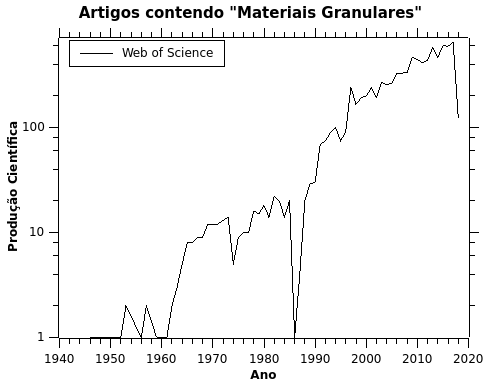
\includegraphics[width=0.8\textwidth]{04-figuras/articles-year.png}
%    \caption{Produção científica acerca de materiais granulares com as palavras chave \textit{"Granular Materials"} ao longo dos anos.}
%    \label{fig:articles-year}
%\end{figure}

\section{Theory}
\label{subsection:Teoria}

%    Como exemplos de materiais granulares temos areia, pedras, solos, fármacos, minérios, alimentos em grãos (arroz, milho, soja, etc.), e até mesmo o cinturão de asteroides e os anéis de Saturno. Só a areia compõe $10\%$ dos materiais da superfície do planeta Terra. Além disso, estima-se que o segundo material mais utilizado nas indústrias são materiais granulares, utilizando aproximadamente $10\%$ de toda a energia do planeta, sendo que o material mais utilizado é a própria água \cite{Sands_Powders_and_Grains}.

    Examples of granular materials includes sand, stones, soils, drugs, ores, grain foods (rice, corn, soybeans, etc.), even the asteroid belt and Saturn's rings. The sand alone makes up $10\%$ of the materials on surface of planet Earth. Besides that, it is estimated that the second most used material in industries are granular materials, using approximately $10\%$ of all the energy on the planet, with the most used material being water itself \cite{Sands_Powders_and_Grains}.

    \begin{figure}
        \begin{minipage}{.45\linewidth}
            \centering
            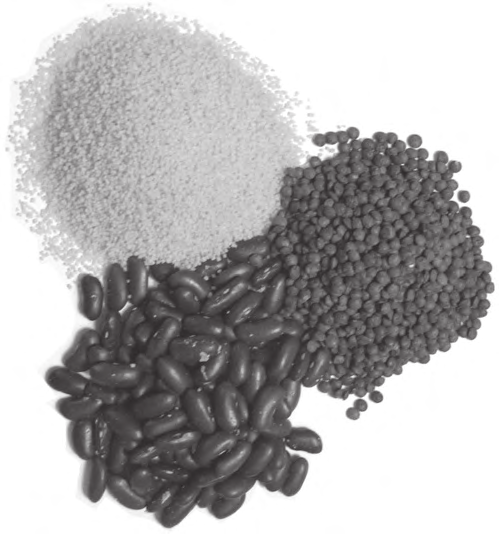
\includegraphics[width=0.9\textwidth]{04-figuras/Exemplo_Alimento.png}
            \subcaption{Grain foods.}
            \label{subfig:exemplo_alimento}
        \end{minipage}
        \begin{minipage}{.45\linewidth}
            \centering
            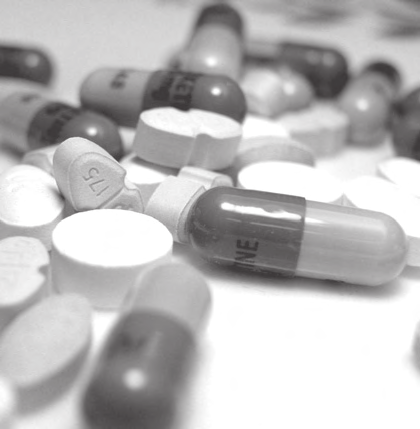
\includegraphics[width=0.9\textwidth]{04-figuras/Exemplo_Medicamento.png}
            \subcaption{Drugs.}
            \label{subfig:exemplo_medicamento}
        \end{minipage}
        \begin{minipage}{.45\linewidth}
            \centering
            \includegraphics[width=0.9\textwidth]{04-figuras/Exemplo_Açucar.png}
            \subcaption{Sugar.}
            \label{subfig:exemplo_acucar}
        \end{minipage}
        \begin{minipage}{.45\linewidth}
            \centering
            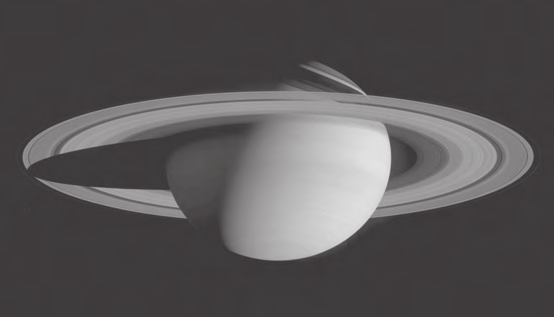
\includegraphics[width=0.9\textwidth]{04-figuras/Exemplo_Saturno.png}
            \subcaption{Saturn and its rings.}
            \label{subfig:exemplo_saturno}
        \end{minipage}
        \caption{Examples of granular material. Figures taken from \cite{Granular_Media_Between_Fluid_and_Solid}.}
    \end{figure}

%    Pela ausência de movimentos Brownianos, bem como pela dissipação de energia, sistemas granulares não sofrem relaxação espontânea de suas configurações estáveis na ausência de perturbações externas, principalmente na forma de vibrações, e portanto não apresentam ergodicidade\footnote{Um sistema ergódico tem característica de transitar entre seus microestados de energia espontaneamente, em intervalos de tempos, implicando que seus estados são todos equiprováveis quando analisados em um longuíssimo tempo \cite{Dissertacao, Srdjan-Tese, Granular_Solids_Liquids_and_Gases}.}.

    Due to the absence of Brownian movements, as well as the dissipation of energy in the contact, granular systems does not undergo spontaneous relaxation of its stable configurations in the absence of external disturbances, and therefore do no have ergodicity\footnote{An ergodic system has the characteristic of moving between their micro-states of energy spontaneously, in intervals of time, implying that their states are all equiprobable when analyzed in a very long time \cite{Srdjan-Tese, Unifying_Concepts_in_Granular_Media_and_Glasses}.}.

    To demonstrate this non-ergodicity, we can think about a dry sand pile that rests at a base. If this base does not oscillate, the structure of the pile does not change, the structure of internal forces will remain unchanged, even if it is heated or cooled. This means that sand grains cannot transit between all equipotential states spontaneously, and than this sand pile will rest with internal configurations (chain-forces, stress tensors, grain contact, etc.) unchanged. In the section \ref{subchap:Fenomenologia}, one can find more details.

%    Materiais granulares apresentam também particularidades quanto às suas fases. Apresentam-se individualmente em corpos sólidos, e quando o conglomerado está próximo do repouso, constituem a fase sólida do sistema. Porém, se o sistema é agitado, ou configurado além de um limiar crítico do ângulo de repouso, pode apresentar-se nas fases de granular líquido\footnote{Granulares líquidos podem possuir uma camada limite que flui sobre a camada sólida do sistema.} ou granular gasoso. Tal classificação ainda está em aberto na literatura, apesar de existirem proposições para o que seria a temperatura granular do sistema \cite{Granular_Solids_Liquids_and_Gases}.

    Granular materials also have particularities regarding their phases, analogously to the state of matter. They are presented individually in solid bodies, and when the conglomerate is close to rest, they constitute the equivalent solid phase of the state of matter. However, if the granular system is slightly agitated, or configured beyond a critical threshold of angle of rest, it can be interpreted in similarity of the liquid state of matter\footnote{Liquid granules can have a boundary layer that flows over the sold layer of the system.}. Granular gases are granular systems that are vigorously agitated, with low packing fraction\footnote{Packing fraction is the measure of the occupied space by the solid portion in relation of the total space.}, and they tend to occupy a large part of the recipe which contains them. An example of the granular state is shown in figure \ref{fig:exemplo_fases}, where the solid phase is static in the bottom, the liquid phase is flowing though layers in the middle, and the gaseous phase is flowing in a higher disordered portion at top. Such classification is still open in the literature, although there are proposals for what would be the granular temperature of the system, in analogous of thermal temperature \cite{Granular_Solids_Liquids_and_Gases}.

    \begin{figure}
        \centering
        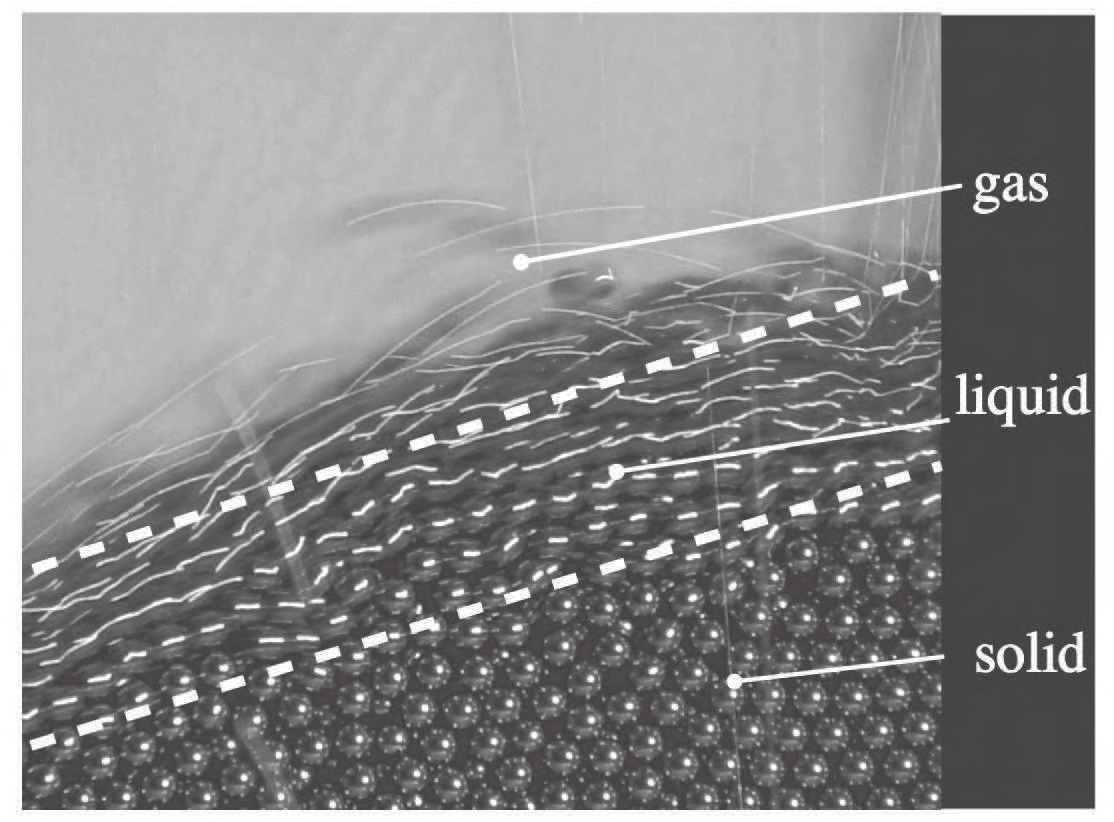
\includegraphics[width=0.9\textwidth]{04-figuras/Exemplo_Fases.png}
        \label{fig:exemplo_fases}
        \caption{Example of three granular phases according their kinetic energy. Figures taken from \cite{Granular_Media_Between_Fluid_and_Solid}.}
    \end{figure}

%    Uma diferenciação entre sistemas granulares pode ser resultado direto das forças de interações entre os grãos. São chamados de granulares secos os sistemas que possuem apenas interações repulsivas, enquanto os granulares molhados apresentam forças de van der Waals nas interações grão a grão. Nesta tese, consideraremos apenas as interações repulsivas de contato, apesar de que em alguns casos, existe fluido envolvendo o material. Consideramos que todo o material que está envolvido pelo mesmo fluido não sofre forças de atração entre os mesmos grãos, e portanto, não está inclusa força de van der Waals na interação entre os grãos.

    A differentiation between granular systems can be a direct result of the interaction forces between grains. Systems that have only repulsive interactions are called dry granulars, while wet granulars have van der Waals forces in grain-to-grain interactions. In this thesis, we will only consider repulsive contact interactions, although in some cases, there is fluid surrounding the material. We consider that all the material that is involved by the same fluid does not suffer forces of attraction between the same grains, and therefore, van der Waals force is not included in the interaction between the grains.

\section{Fenomenologia de Materiais Granulares}
\label{subchap:Fenomenologia}

%Pilha de areia
    Talvez a primeira ideia sobre materiais granulares remeta ao empilhamento de areira. Nesse caso, tem-se uma pilha estática de areia\footnote{A pilha estática está no estado sólido da fase granular \cite{Granular_Solids_Liquids_and_Gases}.}, amontoada sobre uma superfície. Note que em uma pilha como essa, os grãos sempre atingem uma determinada altura, e quando coloca-se mais material sobre a pilha, em algum momento, as camadas superiores da pilha escorrem até a base. Sempre que a pilha ultrapassar o ângulo crítico de repouso \cite{Granular_Physics}, ocorrerá uma avalanche, restaurando o sistema a um outro ângulo característico. Esta propriedade é a de auto-organização\footnote{Um sistema que não possui controlador central, regido por vários agentes que interagem entre si, com regras conhecidas na interação dos agentes e exibem propriedade não prevista pelas interações entre os agentes caracterizam um Sistema Complexo. Uma propriedade característica de Sistemas Complexos e de materiais granulares é a auto-organização. Alguns autores \cite{Mixing_and_Segregation_of_Granular_Materials, Measuring_the_flowing_properties_of_powders_and_grains, Revisiting_localized_deformation_in_sand_with_complex_systems, Granular_matter_and_networks, Patterns_and_collective_behavior_in_granular_media} classificam materiais granulares dentro da área de estudo de Sistemas Complexos.} da pilha de areia pelo ângulo crítico de repouso. Uma boa aproximação do ângulo de repouso é dada pela equação \ref{equ:atrito}:
\begin{equation}
    \label{equ:atrito}
    tan(\theta) = \mu _s ,
\end{equation}
onde $\theta$ é o ângulo crítico de repouso, e $\mu _s$ é o coeficiente de atrito do material.

%Biestabilidade da pilha
    Um pouco mais curioso ainda sobre as pilhas de grãos é que o histórico de preparação do sistema reflete-se no ângulo de repouso \cite{Dynamics_at_the_angle_of_repose}. Este histórico de preparação permite o sistema configurar-se diferentemente, e portanto, o ângulo de repouso assume valores diferentes utilizando o mesmo material. Existe então um ângulo de repouso mínimo $\theta _r$, e um ângulo máximo $\theta _m$, em que o empilhamento pode configurar-se: $\theta _r < \theta < \theta _m$ \cite{Granular_Physics}. Ter uma faixa de ângulos estáveis entre o ângulo mínimo de repouso e o ângulo máximo recebe o nome de biestabilidade do ângulo de repouso.

%Diferentes preparações, diferentes pressões
    Uma evidência de que o histórico de preparação altera a configuração do material é descrita nos artigos "\textit{Sensitivity of Stress Response Function to Packing Preparation}" e "\textit{Memories in sand: Experimental tests of construction history on stress distributions under sandpiles}" \cite{Sensitivity_of_Stress_Response_Function_to_Packing_Preparation, Memories_in_Sand}. A base circular apresentada na figura \ref{fig:pile_stress} foi feita com duas formas de deposição diferentes. No experimento, a pressão medida na base varia de acordo com a deposição, sendo que a deposição feita a partir do funil possui um pico de máximo de pressão em torno de $0,25$ e $0,5$ do raio da mesa, enquanto na deposição feita a partir da peneira apresenta pressão como espécie de platô entre o centro da mesa e $0,25$ do raio, com o máximo próximo do centro.

\begin{figure}
    \centering
    \begin{minipage}{.45\linewidth}
        \centering
        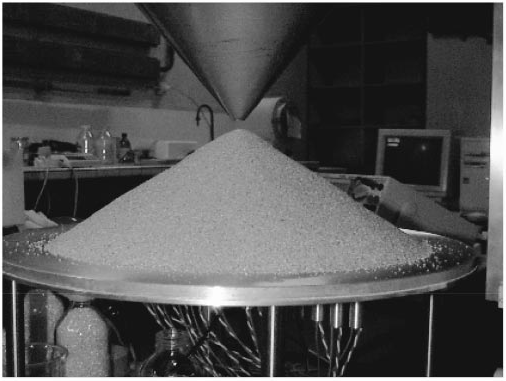
\includegraphics[width=0.9\textwidth]{04-figuras/Sand_Pile_GG_Experiment.png}
        \subcaption{Empilhamento a partir do funil.}
        \label{fig:pressure_pile:GG}
    \end{minipage}
    \begin{minipage}{.45\linewidth}
        \centering
        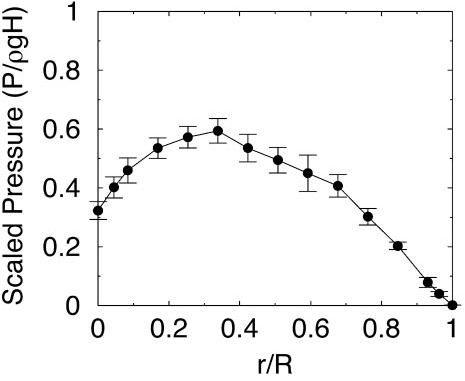
\includegraphics[width=0.9\textwidth]{04-figuras/Sand_Pile_GG_Pressure.png}
        \subcaption{Pressão na montagem a partir do funil.}
        \label{fig:pressure_response:GG}
    \end{minipage}
    \begin{minipage}{.45\linewidth}
        \centering
        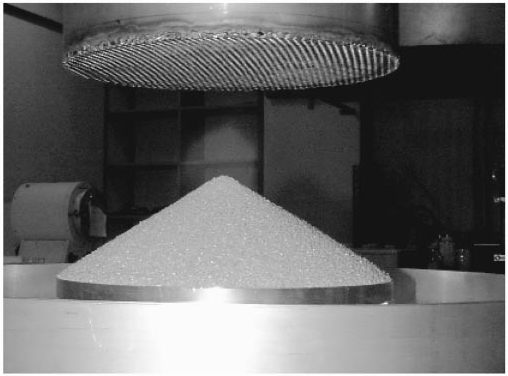
\includegraphics[width=0.9\textwidth]{04-figuras/Sand_Pile_RL_Experiment.png}
        \subcaption{Empilhamento a partir da peneira.}
        \label{fig:pressure_pile:RL}
    \end{minipage}
    \begin{minipage}{.45\linewidth}
        \centering
        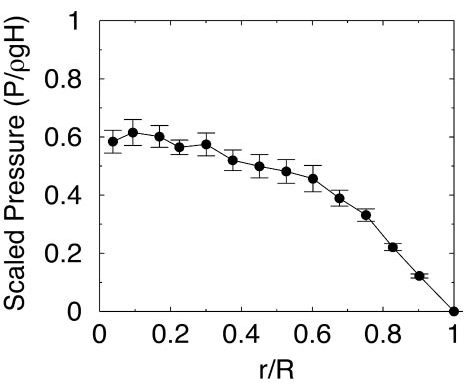
\includegraphics[width=0.9\textwidth]{04-figuras/Sand_Pile_RL_Pressure.png}
        \subcaption{Pressão na montagem a partir da peneira.}
        \label{fig:pressure_response:RL}
    \end{minipage}
    \caption{A preparação das pilhas de areia reflete nas pressões medidas na base da pilha. Nas figuras \ref{fig:pressure_pile:GG} e \ref{fig:pressure_response:GG} a deposição a partir do funil cria um perfil de pressões que tem o pico fora do centro da pilha, enquanto nas figuras \ref{fig:pressure_pile:RL} e \ref{fig:pressure_response:RL} a deposição a partir da peneira cria um perfil de pressões que tem um platô e depois decai. Figuras retiradas de \cite{Memories_in_Sand}.}
    \label{fig:pile_stress}
\end{figure}    

%Função resposta em diferentes configurações
    Um estudo feito por Atman \textit{et al.} \cite{Sensitivity_of_Stress_Response_Function_to_Packing_Preparation} mostra que diferentes geometrias de materiais granulares resultam em diferentes funções respostas\footnote{Função resposta é a diferença entre duas configurações, uma antes de aplicar-se a carga de teste e após a aplicação da carga, mostrando-se a distribuição de forças sobre o material, ou a compressão do sistema \cite{The_Physics_of_Granular_Media}.}. Como exemplo, a figura \ref{fig:stress_response} mostra duas funções respostas para sistemas com geometria circular e pentagonal.

\begin{figure}
    \centering
    \begin{minipage}{.45\linewidth}
        \centering
        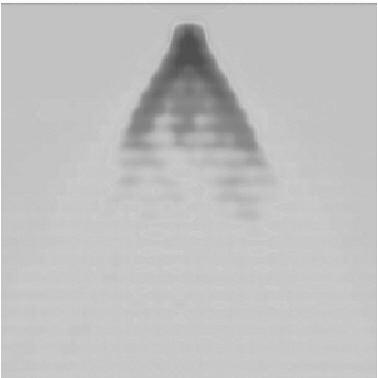
\includegraphics[width=0.9\textwidth]{04-figuras/Funcao_Resposta1.png}
        \subcaption{Grãos circulares.}
        \label{fig:stress_response:circle}
    \end{minipage}
    \begin{minipage}{.45\linewidth}
        \centering
        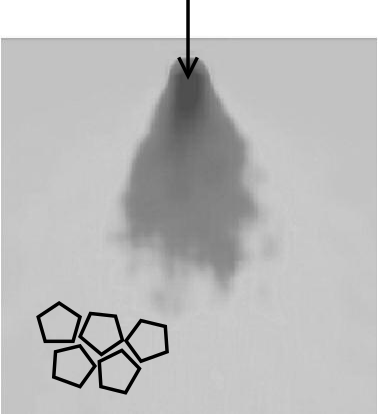
\includegraphics[width=0.9\textwidth]{04-figuras/Funcao_Resposta2.png}
        \subcaption{Grãos pentagonais.}
        \label{fig:stress_response:pentagon}
    \end{minipage}
    \caption{A aplicação de uma força em diferentes sistemas granulares resulta em diferentes funções respostas. A diferença entre estes sistemas é que a figura \ref{fig:stress_response:circle} possui grãos de geometria circular e possui maior ordem, enquanto a figura \ref{fig:stress_response:pentagon} possui geometria pentagonal e maior desordem. Figuras retiradas de \cite{Sensitivity_of_Stress_Response_Function_to_Packing_Preparation}.}
    \label{fig:stress_response}
\end{figure}

%Cadeias de forças em diferentes pilhas
    Já que citamos as diferentes funções respostas nos empilhamentos de grãos, não podemos deixar de citar as cadeias de forças\footnote{Cadeias de forças consistem na rede de contatos entre os grãos que possuem força acima da força média do sistema. Em geral, mede-se as cadeias de forças são medidas a partir da função resposta \cite{The_Physics_of_Granular_Media}.}. A importância experimental da visualização das cadeias de forças se dá no entendimento da distribuição das forças internas que sustentam o material. Como exemplo, a figura \ref{fig:force_chain} indicia a cadeia de forças associada à função resposta de uma força puntual aplicada sobre o topo do material granular.

\begin{figure}
    \centering
    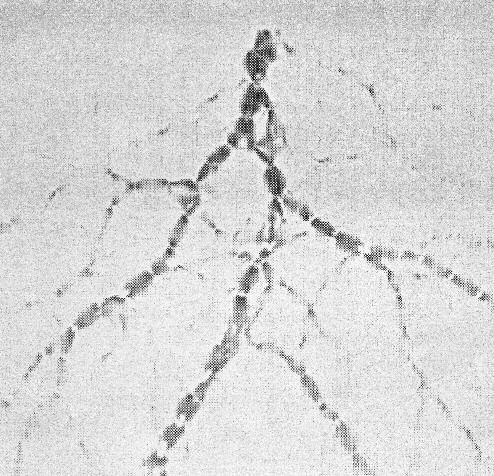
\includegraphics[width=0.5\textwidth]{04-figuras/Cadeia_Forca.png}
    \caption{A aplicação de uma força puntual no topo do material resulta na cadeia de forças, que pode ser vista através da função resposta do sistema. Neste caso, o sistema é preparado com grãos fotoelásticos em uma distribuição bidimensional. Quanto mais escuras, maiores são as tensões no material. Figura retirada de \cite{Sensitivity_of_Stress_Response_Function_to_Packing_Preparation}.}
    \label{fig:force_chain}
\end{figure}

%Formação de arcos
    As cadeias de forças são importantes para entender o fenômeno que está presente nos arcos de sustentação que utilizamos. Arcos são estruturas coletivas que possuem sustentação mútua, e, consequentemente, uma cadeia de forças ligando toda a estrutura, sendo capaz de sustentar o peso próprio e de todos os grãos acima, impedindo que os mesmos escoem. Na formação de arcos podem ocorrer efeitos de segregação, como verificado por Magalhães, C. e Magalhães, F. \cite{Caio-Tese, Felipe-Tese}.

%Pressão e tensão
    As medidas em materiais granulares geralmente tentam caracterizar o material em duas escalas diferentes que se relacionam: microescala, que diz respeito das medidas na escala dos grãos, como atrito; e macroescala, que diz respeito das medidas na escala do sistema, como pressão e tensão de cisalhamento.

%Dilatação
    Uma curiosidade sobre os materiais granulares é que quando estão submetidos a uma pressão e seu coeficiente de compactação\footnote{\label{foot:packingfraction}O coeficiente de compactação é dado pela razão da soma dos volumes individuais dos grãos pelo volume de ocupação no espaço.} está próximo do engarrafamento \cite{Non-Gaussian_behavior_in_jamming_unjamming_transition_in_dense_granular_materials}, uma dilatação tende a ocorrer, expandindo-se pelas bordas das fronteiras que confinam o material ou pelas outras direções de liberdade que o confinamento apresenta. Muitas vezes, ao aplicar-se uma pressão no material confinado, o coeficiente de compactação final pode ser menor que o inicial, indicando uma expansão volumétrica do sistema \cite{Felipe-Tese}.

%Escoamento de granular
    Aproveitando o exemplo do empilhamento, observa-se que na formação da pilha, após os grãos atingem o ângulo critico, ocasiona-se uma avalanche do material. Na avalanche, a camada superior entra em movimento, enquanto as camadas abaixo continuam estáticas. Na movimentação da camada superior, o material granular se apresenta no estado líquido, enquanto a camada estática abaixo encontra-se no estado sólido \cite{Granular_Solids_Liquids_and_Gases}. A figura \ref{fig:inclinacao} exemplifica a transição de fase sólido líquido entre as camadas.

\begin{figure}
    \centering
    \begin{minipage}{.45\linewidth}
        \centering
        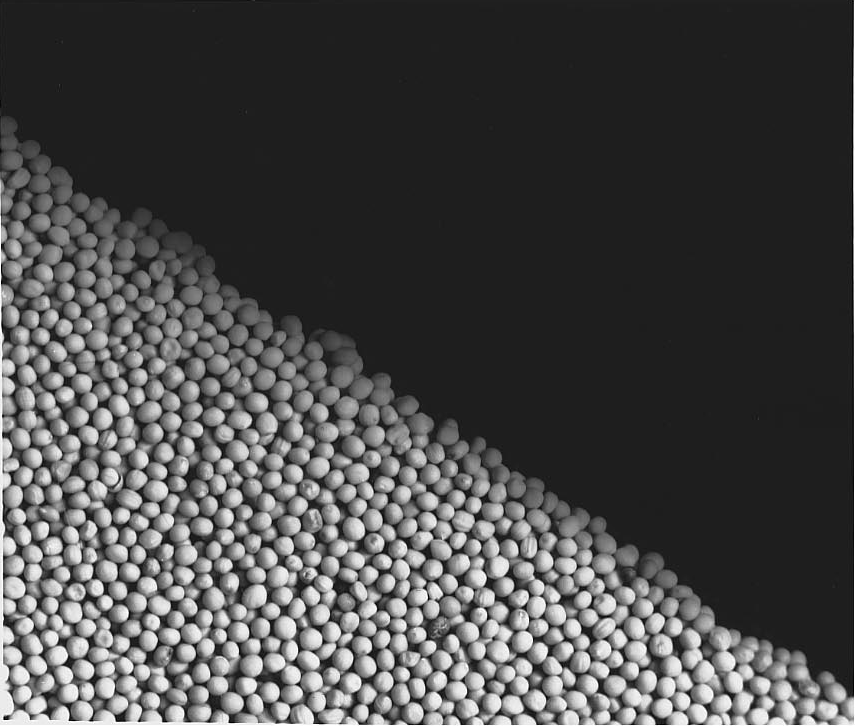
\includegraphics[width=0.9\textwidth]{04-figuras/Pilha1.png}
        \subcaption{Pilha estática.}
        \label{fig:inclinacao:solido}
    \end{minipage}
    \begin{minipage}{.45\linewidth}
        \centering
        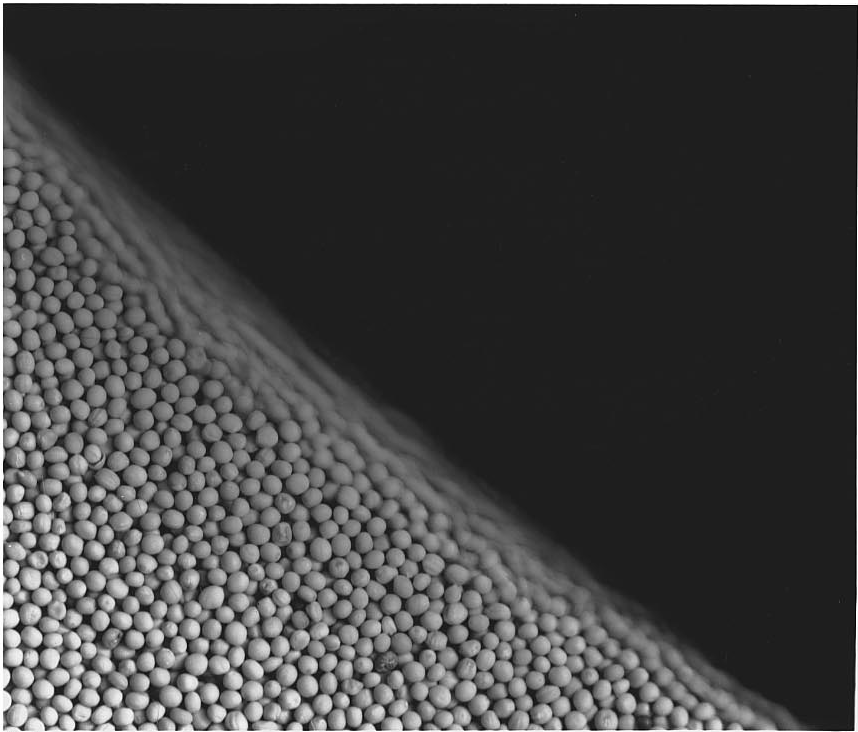
\includegraphics[width=0.9\textwidth]{04-figuras/Pilha2.png}
        \subcaption{Pilha escorrendo.}
        \label{fig:inclinacao:liquido}
    \end{minipage}
    \caption{Com o aumento do ângulo da pilha, nota-se que a camada superior desliza sobre a camada inferior (da figura \ref{fig:inclinacao:solido} para a figura \ref{fig:inclinacao:liquido}). Figuras retiradas de \cite{Granular_Solids_Liquids_and_Gases}.}
    \label{fig:inclinacao}
\end{figure}

    Escoamentos podem ocorrer então por tensões aplicadas no material, seja em uma inclinação da base, seja pela vibração do material. Como a mudança de configurações do material está relacionada a taxa de cisalhamento do material, mas a tensão de cisalhamento não é necessariamente proporcional a taxa de cisalhamento, este escoamento pode ser classificado como fluido não newtoniano.

%Segregação
%    Um fenômeno muito estudado é a segregação dos materiais granulares. O efeito de segregação ocorre em diferentes geometrias de material, densidades e coeficientes de atrito.

%Vibração
%    Vibrações no material granular fornecem energia ao sistema

    No próximo capítulo descreveremos as equações e os procedimentos para realizar as simulações dos materiais granulares, desde o modelo de contatos até a inserção do fluido no sistema.
    % Trabalhos relacionados
\chapter{Discrete Element Method - DEM}
\label{chap:DEM}
    Numerical simulations are widely used to study granular systems, which play an important role in complementing experimental information, which further enhances the understanding of granular physics phenomena. A justification to the use of numerical simulations is the precise control of the input parameters of the simulations and the level of complexity about the object of study. Another advantage is the extraction of data, that goes from the grain scale (microscale), such as positions and velocity of grains, rising to the scale of force chains (mesoscale), up to the system scale (macroscale), such as material shear, showing possible emerging properties and their causes.

    The technique to simulate of granular materials that we use in this work is a DEM known in the literature as Molecular Dynamics (MD). The method consists of numerically solving the Newton's laws of motion. An advantage of this method is that any force that can describe the interaction with the elements is accepted in this method.

    The technique described in the reference \cite{Computer_Simulation_of_Liquids} uses the formalisms of analytical mechanics through the interaction potentials between agents, whether Lagrangian or Hamiltonian potentials, to establish the forces acting on each agent. The disadvantage of this type of description is that dissipative forces may not appear, since the description of forces is directly related to potentials. Formally, the system must obey the set of Equations \label{equ:lagrange} described by the Lagrangian function of the system: 
\begin{subequations}
    \label{equ:lagrange}
    \begin{empheq}[left={}]{align}
        \label{equ:lagrange1}
        \mathcal{L} = \mathcal{T} - \mathcal{V},\\
        \label{equ:lagrange2}
        \sum_{k} \left[\frac{d}{dt} \left( \frac{\partial \mathcal{L}}{\partial \dot{q_k}} \right) - \left(\frac{\partial \mathcal{L}}{\partial q_k} \right)\right] = 0,\\
        \label{equ:lagrange_forca}
        \vec{F}_{i} = \nabla \mathcal{L} = -\nabla \mathcal{V},
    \end{empheq}
\end{subequations}
where $\mathcal{L}$ represents the Lagrangian function that governs the dynamics of the system, $\mathcal{T}$ the kinetic energy, $\mathcal{V}$ the potential energy, $k$ the number of generalized coordinates of the system, $q_{k}$ the generalized coordinates, $\dot{q_{k}}$ the generalized velocities, $\vec{F}_{i}$ the force exerted on the particle $i$ originated by the gradient of the potential $\mathcal{V}$. 

    Other references \cite{Dissertacao, Abraao-Dissertacao, Caio-Tese, Srdjan-Tese, Felipe-Tese, Nathalia-Dissertacao, Leticia-Dissertacao, Fabiola-Dissertacao, Luding-Tese, Caio-Dissertacao, Bouzid-Tese, Wassgren-Tese, Computational_Granular_Dynamics} use the model directly from the acting forces about each element.

\section{Equations of motion}
    To carry out the simulation, the set of Equations \ref{equ:movimento} must be satisfied, which takes into account Newton's laws of motion. Thus, there is information on the agents' states as a function of time. 
\begin{subequations}
    \label{equ:movimento}
    \begin{empheq}[left={Translational}\empheqlbrace]{align}
        \label{equ:posicao_linear}
        \vec{r}_{i}(t) &= \vec{r}_{i}(0) + \int_{0}^{t} \vec{v}_{i}(t) dt,\\
        \label{equ:velocidade_linear}
        \vec{v}_{i}(t) &= \vec{v}_{i}(0) + \int_{0}^{t} \vec{a}_{i}(t) dt,\\
        \label{equ:aceleracao_linear}
        \vec{a}_{i}(t) &= \sum_{j} \frac{\vec{F}_{i,j}(t)}{m_{i}},
    \end{empheq}
    \begin{empheq}[left={Rotational}\empheqlbrace]{align}
        \label{equ:posicao_angular}
        \theta^{k}_{i}(t) &= \theta^{k}_{i}(0) + \int_{0}^{t} \vec{\omega}^{k}_{i}(t) dt,\\
        \label{equ:velocidade_angular}
        \vec{\omega}^{k}_{i}(t) &= \vec{\omega}^{k}_{i}(0) + \int_{0}^{t} \vec{\alpha}^{k}_{i}(t) dt,\\
        \label{equ:aceleracao_angular}
        \vec{\alpha}^{k}_{i}(t) &= {I^{k}_{i}}^{-1} \sum_{j} \vec{\tau}^{k}_{i,j}(t),
    \end{empheq}
\end{subequations}
where $i$ is the i-th particle of the system, $\vec{r}_{i}(t)$ is the position vector of the center of mass of the body $i$ at the instant of time $t$, $\vec{v}_{i}(t)$ or $\vec{\dot{r}}_{i}(t)$ is the velocity vector of the center of mass of the body, $\vec{a}_{i}(t)$ or $\vec{\dot{v}}_{i}(t)$ or $\vec{\ddot{r}}_{i}(t)$ is the vector of accelerations of the center of mass of the body, $\vec{F}_{i,j}(t)$ is the component of the force that the center of mass of the body suffers from interacting with another body or field $j$, $m_{i}$ is the body mass, $\theta^{k}_{i}(t)$ is the basis of the body rotation coordinates expressed in the system's $k$ basis, $\vec{\omega}^{k}_{i}(t)$ is the pseudovector of angular velocities of the body expressed on the basis $k$ of the system, $\vec{\alpha}^{k}_{i}(t)$ is the pseudovector of angular accelerations of the body, ${I^{k}_{i}}^{-1}$ is the inverse of the inertia tensor of the body and $\vec{\tau}^{k}_{i,j}(t)$ is the torque vector that the body suffers from interacting with another body or field. Remembering that the relationship between torque and the force that causes it can be described by the Equation \ref{equ:torque}:
\begin{equation}
    \label{equ:torque}
    \vec{\tau}_{i,j}(t) = \vec{\chi}_{i,j}(t) \times \vec{F}_{i,j}(t),
\end{equation}
where the vector $\vec{\tau}_{i,j}(t)$ is the torque on the particle $i$ caused by the contact forces with the body or field $j$. The vector $\vec{\chi}_{i,j}(t)$ is the vector that connects the center of mass of the particle $i$ to the point of application of the force, and the vector $\vec{F}_{i,j}(t)$ is the vector of the contact forces caused by interacting with another body or field $j$. The Equations \ref{equ:aceleracao_linear} and \ref{equ:aceleracao_angular} express Newton's second law. 

    The formulation described by the set of Equations \ref{equ:movimento} covers spaces in 1D, 2D and 3D, but this thesis focuses only on the formulation of 2D systems.

\subsection{Force model}
\label{subchap:Modelo_Forcas}
    The forces present in the systems modelled in this Chapter include the contact forces between agents and the gravitational force. The interaction forces between grain and fluid is described in Chapter \ref{chap:CFD}.

\subsubsection{Contact forces}
\label{subsubchap:Reologia}
    The contact forces model between grains we used to simulate granular materials was the rheological model proposed by Kelvin-Voigt \cite{Kelvin, Voigt}. Kelvin-Voigt rheology models the contact force between two grains by a spring and a damper in parallel in the normal direction of contact, as exemplified in Figure \ref{fig:forcas}. The normal spring represents the elastic contribution of the material, related to the Young's modulus, while the normal damper has the function of dissipate the energy in the inelastic collision between the grains. Additionally, a tangential spring is inserted in the tangential direction to play the role of the Coulomb friction. A model proposed in \cite{Caio-Tese} adds a damper-like element in parallel to the tangential spring, modelling the rolling resistance. We chose to use circular geometry for the grains. In consequence of the circular geometry, all angular momentum variation is caused by torque due to tangential force.

\begin{figure}
    \begin{minipage}{.45\linewidth}
        \centering
        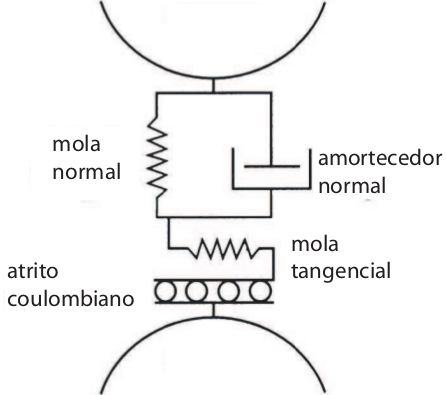
\includegraphics[width=0.9\textwidth]{04-figuras/Modelo_Forcas.png}
        \subcaption{Contact force model between agents. }
        \label{fig:forcas_modelo}
    \end{minipage}
    \begin{minipage}{.45\linewidth}
        \centering
        \includegraphics[width=0.9\textwidth]{04-figuras/Contato.tikz}
        \subcaption{Contact representation between grains.}
        \label{fig:forcas_contato}
    \end{minipage}
    \caption[Contact force model.]{Force model and representation between two circular grains. Figures taken from \cite{Sands_Powders_and_Grains}.}
    \label{fig:forcas}
\end{figure}

    A peculiarity of DEM is that it allows interpenetration between the grains. Therefore, in this model there is no deformation when two bodies are in contact. The maximum interpenetration we allow in our model is controlled by the material's hardness parameter and we impose a maximum penetration of $0.5\%$ of the radius.

    To determine the value of the interpenetration, $\delta$, in circular geometry, the Equation \ref{equ:interpenetracao}:
\begin{equation}
    \label{equ:interpenetracao}
    \delta_{i,j}^{\perp} = \left(R_{i}+R_{j}-\left|\vec{r}_{j}-\vec{r}_{i}\right|\right)\mathcal{H}(R_{i}+R_{j}-\left|\vec{r}_{j}-\vec{r}_{i}\right|),
\end{equation}
where $\delta_{i,j}^{\perp}$ is the value of the interpenetration between the grains $i$ and $j$, $R_{i}$ is the radius of the body $i$, $R_{j}$ is the radius of the body $j$, $\vec{r}_{i}$ is the position vector of the center of the body $i$, $\vec{r}_{j}$ is the position vector of the center of the body $j$ and $\mathcal{H}$ is the Heaviside step function. So, when the distance between the bodies is greater than the sum of the radii, the bodies will not be in contact and the Heaviside step function indicates that the interpenetration between the grains is null. If the distance between the bodies is lesser than the sum of the radii, the bodies will be in contact and the Heaviside step function indicates that there is interpenetration between grains, by its value being equals to one.

    With grains being in contact, the direct consequence of the interpenetration is the appearance of an elastic repulsive force, and the force depends on the interpenetration function $\delta^{\perp}$. The force expression can be calculated by the Equation \ref{equ:forca_elastica}: 
\begin{equation}
    \label{equ:forca_elastica}
    \vec{F}_{i,j}^{el} = -k_{n}\left(\delta_{i,j}^{\perp}\right)^{\frac{D}{2}}\hat{n}_{i,j},
\end{equation}
where $\vec{F}_{i,j}^{el}$ is the normal elastic force that the body $j$ causes to the body $i$ when they come in contact, $k_{n}$ is the constant related to the elasticity of the material in the direction of contact, $\delta_{i,j}^{\perp}$ is the interpenetration between the bodies $i$ and $j$, $D$ is the dimension of the system (in this case, $D=2$) and $\hat{n}_{i,j}$ is the normal direction of the contact \cite{Dissertacao, Caio-Tese, Landau}. One can write a potential for this elastic force as: $\mathcal{V} = \frac{1}{2}k_{n}\left({\delta_{i,j}^{\perp}}\right)^2$.

    Associated with the elastic force, the damping force is also present. As it is a dissipative force, a potential cannot be associated with the damping force. Most of the energy loss of granular materials is in collision. The Equation \ref{equ:forca_amortecimento} describes its behavior: 
\begin{equation}
    \label{equ:forca_amortecimento}
    \vec{F}_{i,j}^{am} = -\gamma \left(\vec{v}_{i,j}.\hat{n}_{i,j}\right)\hat{n}_{i,j},
\end{equation}
where $\vec{F}_{i,j}^{am}$ is the normal damping force that the body $j$ causes to the body $i$ when they come in contact, $\gamma$ is the damping constant related to the inelastic collision, $\vec{v}_{i,j}$ is the relative velocity between the centers of mass of bodies $i$ and $j$ and $\hat{n}_{i,j}$ is the normal contact direction \cite{Dissertacao, Caio-Tese, Computational_Granular_Dynamics}.

    The damping constant is directly linked to the restitution coefficient and can be used equivalently through the identities shown in the set of Equations \ref{equ:restituicao}. Some authors use the restitution coefficient in simulations, such as \cite{Srdjan-Tese, Luding-Tese, Computational_Granular_Dynamics}. In this thesis we will use the damping coefficient.

\begin{subequations}
    \label{equ:restituicao}
    \begin{empheq}[left={}]{align}
        \epsilon &= \exp\left(\frac{-\pi}{\sqrt{\frac{4k_{n}m}{\gamma^2}-1}}\right),\\
        \gamma &= \sqrt{\frac{4k_{n}m}{\left(\frac{\pi}{\ln\left(\epsilon\right)}\right)^2+1}},
    \end{empheq}
\end{subequations}
where $\epsilon$ is the restitution coefficient, $\gamma$ is the damping coefficient, $k_{n}$ is the stiffness related to the elasticity of the material and $m$ is the reduced mass $m=\frac{m_{i}m_{j}}{m_{i}+m_{j}}$.

    The friction force is also present in the simulation model. As the surfaces are in contact, there will be a frictional force between them if they tend to move each other. In particular, due to the circular geometry, friction forces will only act in the tangential direction. The relative velocity between the contact point of the bodies is given by the Equation \ref{equ:velocidade_relativa} below: 
\begin{equation}
    \label{equ:velocidade_relativa}
    \delta_{i,j}^{\parallel} = \vec{v}_{ij}.\hat{t}_{ij} - R_{i}\omega_{i} - R_{j}\omega_{j},
\end{equation}
where $\delta_{i,j}^{\parallel}$ is the relative velocity of the contact point of the bodies $i$ and $j$, $\vec{v}_{ij}$ is the relative velocity of the centers of mass of the bodies $i$ and $j$, $\hat{t}_{ij}$ is the tangential vector to the contact surfaces of the bodies $i$ and $j$, $R_{i}$ is the radius of the body $i$, $R_{j}$ is the radius of the body $j$, $\omega_{i}$ is the angular velocity of the body $i$ and $\omega_{j}$ is the angular velocity of the body $j$.

    For the tangential force, it is necessary to know the relative displacement of the contact point, as given by the equation \ref{equ:velocidade_relativa}, applied in the system of Equations \ref{equ:forca_atrito}, which models the Coulomb friction, and is given by:
\begin{equation}
    \label{equ:forca_atrito}
    \vec{F}_{i,j}^{at} = \left\{
    \begin{array}{l l l}
        \displaystyle -\int_{t_{0}}^{t_{f}} k_{t} \delta_{i,j}^{\parallel} \hat{t}_{ij}\, \mathrm{d} t, & \quad \textrm{if } k_{t} \left| \delta_{i,j}^{\parallel} \right| \leq \mu \left|\vec{F}_{i,j}^{n}\right| & \textrm{ (Static friction)} \\
        \displaystyle -\frac{\delta_{i,j}^{\parallel}}{\left|\delta_{i,j}^{\parallel}\right|} \mu \left| \vec{F}_{i,j}^{n} \right| \hat{t}_{ij}\, & \quad \textrm{if } k_{t} \left| \delta_{i,j}^{\parallel} \right| > \mu \left| \vec{F}_{i,j}^{n} \right| & \textrm{ (Kinetic friction)}
    \end{array}
    \right.\ ,
\end{equation}
where $\vec{F}_{i,j}^{at}$ is the friction force between the bodies $i$ and $j$, $k_{t}$ is the elastic constant of the material in the tangential direction, $\delta_{i,j}^{\parallel}$ is the relative velocity between the contact point of the bodies $i$ and $j$, $\hat{t}_{ij}$ is the tangential vector to contact surfaces of bodies $i$ and $j$, $\mu$ is the friction coefficient between the surfaces of bodies $i$ and $j$ and $\vec{F}_{i,j}^{n} = \vec{F}_{i,j}^{el} +\vec{F}_{i,j}^{am}$ is the force normal to the surfaces of bodies $i$ and $j$.

    We chose to model static and dynamic friction coefficient to be a single value for simplicity, presented the friction coefficient $\mu$. Figure \ref{fig:atrito} describe the Coulomb friction we use in the simulations.

\begin{figure}
    \centering
    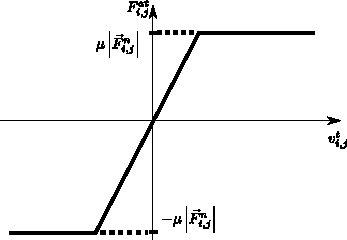
\includegraphics[width=0.5\textwidth]{04-figuras/Atrito.pdf}
    \caption[Friction.]{Friction versus relative velocity between contact. Figure taken from \cite{Caio-Tese}.}
    \label{fig:atrito}
\end{figure}

\subsubsection{The external force: Gravity}
\label{subsubchap:Gravidade}
    For this model, we assume that the gravitational force is a constant. For convenience, we normalize gravity as a unit value.

\subsection{The external force: The vibration}
    In the BNE problems, vibration must be present to agitate grains. One way to impose the vibration is to modulate an oscillatory force in the base where grains are. We chose to impose the variation in the position of walls instead of impose this variation in the force that sustains the walls.

\subsection{Temporal discretization}
    For the computational simulation of solid bodies, the kinematics equations must be rewritten as Taylor series expansions, and we chose the interpolating the velocity equation system by the algorithm known as Velocity Verlet \cite{Verlet, Computer_Simulation_of_Liquids}. The equations of motion discretized in time, as a function of the time step $\Delta t$, become as in the set of equations \ref{equ:movimento_discreto}:
\begin{subequations}
    \label{equ:movimento_discreto}
    \begin{empheq}[left={Translational}\empheqlbrace]{align}
        \label{equ:posicao_linear_discreta}
        {\vec{r}_{i}}^{\;n+1} &= {\vec{r}_{i}}^{\;n} + {\vec{v}_{i}}^{\;n} \Delta t + \frac{{\vec{a}_{i}}^{\;n}}{2} (\Delta t)^{2},\\
        \label{equ:velocidade_linear_discreta}
        {\vec{v}_{i}}^{\;n+1} &= {\vec{v}_{i}}^{\;n} + \frac{{\vec{a}_{i}}^{\;n}+{\vec{a}_{i}}^{\;n+1}}{2} \Delta t,\\
        \label{equ:aceleracao_linear_discreta}
        {\vec{a}_{i}}^{\;n+1} &= \frac{\sum_{j} {\vec{F}_{i,j}}^{\;n+1} + \sum {\vec{F}_{i,ext}}^{\;n+1}}{m_{i}},
    \end{empheq}
    \begin{empheq}[left={Rotational}\empheqlbrace]{align}
        \label{equ:posicao_angular_discreta}
        {\theta_{i}}^{n+1} &= {\theta_{i}}^{n} + {\vec{\omega}_{i}}^{\;n} \Delta t + \frac{{\vec{\alpha}_{i}}^{\;n}}{2} (\Delta t)^{2},\\
        \label{equ:velocidade_angular_discreta}
        {\vec{\omega}_{i}}^{\;n+1} &= {\vec{\omega}_{i}}^{\;n} +\frac{{\vec{\alpha}_{i}}^{\;n}+{\vec{\alpha}_{i}}^{\;n+1}}{2} \Delta t,\\
        \label{equ:aceleracao_linear_discreta}
        {\vec{\alpha}_{i}}^{\;n+1} &= {I_{i}}^{-1} \sum_{j} {\vec{\tau}_{i,j}}^{\;n},
    \end{empheq}
\end{subequations}
where $i$ is the index of the moving body, $j$ is the index of the body in contact with the body $i$, $n$ is the time step, $\vec{r}$ is the position of the body, $\vec{v}$ is the velocity of the body, $\vec{a}$ is the acceleration of the body, $\Delta t$ is the size of the time step, $\vec{F}_{i,j}$ is the contact force between the bodies $i$ and $j$, $\vec{F}_{ext}$ are the external forces, such as gravity, $m$ is the mass of the body, $\theta$ is the angular position of the body, $\vec{\omega}$ is the angular velocity of the body, $\vec{\alpha}$ is the angular acceleration of the body, $\vec{\tau}$ is the torque on the body, $I$ is the moment of inertia of the body. 

    The set of Equations \ref{equ:movimento_discreto} is written for the 2D system, since there is only one degree of freedom for the rotation, and consequently all equations are written as a function of a single parameter. The velocity approximation as the weighting between the accelerations in the current and future instants of time is the key to the minimization of the imprecision generated by the discretization \cite{Computer_Simulation_of_Liquids}.

\section{Algorithm}
    In addition to the equations that govern the system, a series of procedures must be carried out so that the simulation can take place. Each of these steps are essential for the simulation to take place, and are dependent on each other. The Algorithm \ref{alg:MD} determines the routines for executing the simulation. We use the 3rd order Gear Predictor-Corrector with the Velocity Verlet to perform the simulations \cite{Computer_Simulation_of_Liquids}.

\begin{algorithm}
    \SetKwInOut{Input}{Entrada}\SetKwInOut{Output}{Saída}
    \Input{configuração de dados inicial da simulação}
    \Output{resposta e medições de simulação ao longo do tempo}
    \While{não atingida a condição de parada da simulação}{
        \If{chegou a hora de listar os Vizinhos}{
            Determinar a lista de corpos Vizinhos\;
        }
        Preditor\;
        Detectar Contatos\;
        Cálculo de Forças\;
        Corretor\;
        \If{Possui Fluido}{
            Cálculo do Fluido\;
        }
    }
    \caption{Dadas as entradas do problema, como posições iniciais dos corpos, velocidades e acelerações, o algoritmo de Dinâmica Molecular monta uma lista de corpos que são vizinhos delimitados por uma certa região, então prediz a posição e a velocidade dos corpos no próximo instante de tempo, procura os contatos que foram formados com a predição, calcula as forças entre cada corpo em contato e inclui as forças externas, corrige as predições de velocidade e aceleração de cada corpo e calcula a dinâmica do fluido. Assim um passo de Dinâmica Molecular é construído. Retirado de \cite{Dissertacao}.}
    \label{alg:MD}
\end{algorithm}


    The algorithm stop condition depends on the purpose of the simulation. Some examples, such as static pile stability, energy fluctuations, breaking of force chains, average system velocity, number of time steps, among several other measurable parameters within the simulation can become the stopping criteria of the simulation. In this thesis, we use the number of simulation time steps as the main stopping criterion. 

    We will briefly discuss each of the routines Algorithm \ref{alg:MD}. For more details, the references \cite{Dissertacao, Computer_Simulation_of_Liquids, Computational_Granular_Dynamics} have further explanations about the routines, with examples and detailed algorithms. 

\subsection{Neighbors}
    The Neighbor-Finding algorithm (Algorithm \ref{alg:vizinhos}) presented here is not in the simplest form, but we chose the most efficient, and it is described in \cite{Dissertacao}. It consists of creating a list of all bodies that belong to a certain region of possible interaction. Creating the list minimizes the number of comparisons during execution, which provides the highest computational performance. The article "Methods of parallel computation applied on granular simulations" \cite{Methods_of_Parallel_Computation_Applied_on_Granular_Simulations} reveals the differences between some methods of creating lists of interacting bodies. This article was written during the preparation of this thesis project and is presented in the Appendix \ref{chap:Artigo}. The Algorithm \ref{alg:vizinhos} refers to the creation of a list of bodies that have the possibility of interacting with each other.

\begin{algorithm}
    \SetKwInOut{Input}{Entrada}\SetKwInOut{Output}{Saída}
    \KwIn{posição dos corpos}
    \KwOut{lista de Vizinhos}
    Dividir o espaço em regiões\;
    \ForEach{corpo}{
        Inserir o corpo na lista da região que pertence\;
        Inserir o corpo nas listas adjacentes da região que pertence\;
    }
    \caption{Algoritmo para criação da lista de corpos vizinhos. Retirado de \cite{Dissertacao}.}
    \label{alg:vizinhos}
\end{algorithm}


\begin{figure}
    \centering
    \includegraphics[width = 0.40\textwidth]{04-figuras/Vizinhos.tikz}
    \caption[Neighbor search.]{The neighbour search in Algorithm \ref{alg:vizinhos} occurs between bodies with their immediate adjacent neighborhood region. Figure taken from \cite{Dissertacao}.}
    \label{fig:vizinhos}
\end{figure}

    The figure \ref{fig:vizinhos} shows the regions that the marked body should be listed. For more details, see the references \cite{Dissertacao, Computer_Simulation_of_Liquids}. 

\subsection{Predictor}
    The prediction routine updates the positions and velocities of the bodies, allowing all forces to be calculated based on the new values. In the set of Equations \ref{equ:movimento_discreto}, equations involving terms with index $n$ are updated in this routine. The \ref{alg:preditor} algorithm shows the structure of the prediction routine.

\begin{algorithm}
    \SetKwInOut{Input}{Input}\SetKwInOut{Output}{Output}
    \Input{positions, velocities, accelerations and the time step $\Delta t$}
    \Output{positions, part of the velocities}
    \ForAll{bodies}{
        Calculate new postions\;
        Predict new velocities\;
    }
    \caption[Predictor.]{Prediction routine for state variables of bodies. Algorithm taken from \cite{Dissertacao}.}
    \label{alg:preditor}
\end{algorithm}


\subsection{Detect contacts}
    The contact detection routine uses the list of neighbors generated by the Algorithm \ref{alg:vizinhos} to check whether the listed body/neighbor pair has interpenetration, described in equation \ref{equ:interpenetracao}, and then generates a new list of bodies that interpenetrate each other to be used in the Algorithm \ref{alg:forcas}. The Algorithm \ref{alg:contatos} describes this operation.

\begin{algorithm}
    \SetKwInOut{Input}{Input}\SetKwInOut{Output}{Output}
    \Input{Neighbor list}
    \Output{Contact list}
    \ForAll{neighbor bodies}{
        Calculate the Interpenetration $\delta_{i,j}$ between bodies $i$ and $j$\;
        \If{$\delta_{i,j} > 0$}{
            Insert the pair $i$ and $j$ in the contact list\;
        }
    }
    \caption[Detect contacts.]{Detect contacts routine. Algorithm taken from \cite{Dissertacao}.}
    \label{alg:contatos}
\end{algorithm}


\subsection{Force calculation}
    The routine to calculate the forces uses the contact list generated by the Algorithm \ref{alg:contatos} to calculate the contact forces between the bodies, such as elastic forces (Equation \ref{equ:forca_elastica}), damping forces (Equation \ref{equ:forca_amortecimento}) and friction forces (Equation \ref{equ:forca_atrito}). In addition to contact forces, bodies are subjected to gravitational force. The Algorithm \ref{alg:forcas} contains the execution of the calculation of the forces. 

\begin{algorithm}
    \SetKwInOut{Input}{Input}\SetKwInOut{Output}{Output}
    \Input{positions, velocities and contact list}
    \Output{acting forces and torques in the bodies}
    \ForEach{body}{
        Apply gravity force\;
        \ForEach{body in the contact list}{
            Calculate the normal forces $\vec{N}$\;
            Calculate the rolling forces ${F}^{d}$\;
            \eIf{$|{F}^{d}| < \mu |\vec{N}|$}{
                $\vec{F}^{at} += \vec{F}^{d}\hat{t}$\;
            }{
                $\vec{F}^{at} += \mu \textrm{sign}(\vec{F}^{d}) N\hat{t}$\;
            }
            Calculate torque\;
        }
    }
%    \caption[Force calculation.]{Aqui são calculadas as resultantes das forças em cada corpo. A força $\vec{N}$ é a força normal, contribuição da força elástica $\vec{F}^{el}$ e força de amortecimento $\vec{F}^{am}$ (equações \ref{equ:forca_elastica} e \ref{equ:forca_amortecimento}), $F^{d}$ é a força de rolamento de um corpo sobre o outro, que deve ser comparado com a força de atrito estático máxima $\mu N$. Retirado e adaptado de \cite{Dissertacao}.}
    \caption[Force calculation]{In this routine, the resultant forces are calculated for each body. The force $\vec{N}$ is the normal force, contribution of the elastic force $\vec{F}^{el}$ and the damping force $\vec{F}^{am}$ (Equations \ref{equ:forca_elastica} and \ref{equ:forca_amortecimento}), $F^{d}$ is the rolling force of one body on the other, which must be compared with the maximum static friction force $\mu N$. Algorithm taken from \cite{Dissertacao}.}
    \label{alg:forcas}
\end{algorithm}


\subsection{Corrector}
    The correction routine updates the speeds and accelerations of the bodies. The forces calculated in the force calculation are used here to perform the Velocity Verlet and determine the velocities and accelerations for the next time step. In the set of Equations \ref{equ:movimento_discreto}, the equations involving terms with index $n+1$ are updated in this routine. The Algorithm \ref{alg:corretor} shows the structure of the correction routine.

\begin{algorithm}
    \SetKwInOut{Input}{Entrada}\SetKwInOut{Output}{Saída}
    \Input{resultante das forças e o passo de tempo $\Delta t$}
    \Output{estado dos corpos prontos para o próximo passo de tempo}
    \ForEach{corpo}{
        Calcular as acelerações\;
        Corrigir as velocidades\;
    }
    \caption{Rotina de correção das variáveis dos corpos. Retirado de \cite{Dissertacao}.}
    \label{alg:corretor}
\end{algorithm}


\section{Important parameters}
    Due to the presented force model, some parameters are important for the simulations. As they are governed by difference equations as a function of the temporal parameter, some criteria must be obeyed for the simulation to be stable. These conditions are related to the error propagation when continuous equations are transformed in their discrete version. One of the parameters is the time constant $\Delta t$, which in our simulations has a direct relationship with the oscillation period of the spring mass model (Kelvin-Voigt rheology), given by $\Delta t = \xi \sqrt{m_{min}/k_{n}}$, where $\xi$ is an adjustment value, $m_{min}$ is the smallest mass of the system, and $k_{n}$ is the spring constant. The factors that stabilize the simulations, they must have at least $\xi < $1/10 \cite{Dissertacao, Caio-Tese, Computer_Simulation_of_Liquids}. In this thesis we will use the factor of $1/100$ for BNE systems. 

    Another important parameter is the damping factor $\gamma$, or the restitution coefficient $\epsilon$. Due to the dissipative nature of granular materials, $\epsilon \simeq 0$, which approximates $\gamma \simeq 2\sqrt{k_{n}{m}_{min}}$, because we will have critical regimes in the spring mass equation when we use the smallest mass of the two bodies, and for all others, the damping will be subcritical \cite{Bouzid-Tese, Luding-Tese}. 

    We model the walls for the BNE problem as smooth. The technique we use is to create a virtual body that has only the fixed component that it does a boundary, while it is free to move in the other direction, coinciding to be in the closest position of the free bodies.

    In the next chapter we will describe the Brazil nut Effect (BNE) and how we set up the simulation that leads to this effect.
           % Metodologia DEM
\chapter{Brazil Nut Effect (BNE)}
\label{chap:BNE}
%    Historicamente, o fenômeno conhecido como BNE foi identificado em função das exportações da castanha do Pará em contêineres, por navios, e sempre que chegavam ao destino, observam-se que as maiores castanhas estavam no topo. Inicialmente pensou-se que os comerciantes brasileiros arranjavam as castanhas de modo que as maiores estivessem em cima e, as menores e quebradas em baixo. Após investigação, foi verificado que as castanhas maiores ascendiam devido à vibração que os contêineres sofriam ao longo do transporte \cite{Caio-Tese}.

    Historically, the phenomenon known as BNE was identified in Brazil nut exports, which were taken in containers on ships leaving Brazil, and whenever they arrived at their destination, it was observed that the largest nuts were at the top. Initially it was thought that Brazilian traders arranged the nuts so that the largest were on top and the smaller and broken ones at the bottom. After investigation, it was verified that the larger nuts rise due to the vibration that the containers suffered during transport \cite{Caio-Tese}. 

%    O BNE ocorre quando grãos de diferentes tamanhos se segregam, fazendo com que os grãos maiores se agrupam com grãos maiores, enquanto menores se agrupam com grãos menores. O efeito de segregação pode ser visto quando um sistema é agitado, ou lhe é imposto um ciclo de cisalhado \cite{Size_segregation_of_irregular_granular_materials_captured_by_time-resolved_3D_imaging}. Este fenômeno está associado com a fase granular do sistema. Num sistema granular sólido, o grão maior fica estático. Com o aumento da agitação, o sistema passa para o estado líquido, permitindo que haja movimentação dos grãos no sistema \cite{Why_the_Brazil_nuts_are_on_top}. A movimentação do material ocorre em correntes de convecção que se formam próximas das paredes e pelo preenchimento do espaço anteriormente ocupado pelo grão maior, com o efeito catraca \cite{Inertia_in_the_Brazil_nut_problem, The_water-enhance_Brazil_nut_effect}.

    The BNE occurs when grains of different sizes segregate, causing larger grains segregate from smaller ones. The segregation effect can be seen when a system is shaken, or a shear cycle is imposed \cite{Granular_Physics}. This phenomenon is associated with the granular phase of the system. In a solid-like granular system, the larger grain is static. With agitation, the system changes to a liquid state, allowing the movement of grains in the system \cite{Why_the_Brazil_nuts_are_on_top}. The movement of the material occurs in convection currents that form close to the walls, or with the ratchet effect \cite{Effects_of_convection_and_friction_on_size_segregation_in_vibrated_granular_beds, Scaling_behavior_in_convection-driven_Brazil-nut_effect, Inertia_in_the_Brazil_nut_problem, The_water-enhance_Brazil_nut_effect}, both cases allow small grains fill the space previously occupied by the larger grain, rising the larger grain. Figure \ref{fig:BNE_hejmady_convection} shows the evolution of the convection currents in a confined media. Once smaller grains collectively move to fill the void left by larger grains, smaller grains imped their downward motion; these correlations are at the basis of the observed size segregation. The ratchet effect is the granular solid-like behavior in below larger grains and the granular liquid-like behavior, where larger grains can move. The ratchet effect is also related to the Reynolds dilatancy, since the stress increases and the granular configuration changes.

\begin{figure}
    \centering
    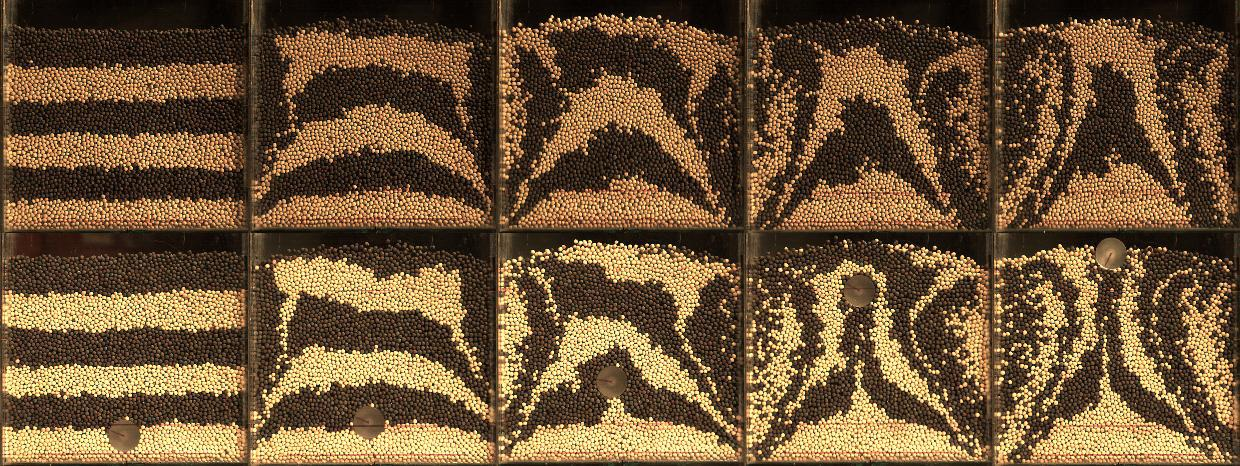
\includegraphics[width=0.65\textwidth]{04-figuras/BNE_Hejmady_Convection.png}
    \caption[Granular convection in vibrated bed.]{Evolution of the vibrated bed. Top Panels are without intruder, while bottom Panels are with an intruder. Black and yellow layers are made of mustard grains. Figure taken from \cite{Scaling_behavior_in_convection-driven_Brazil-nut_effect}.}
    \label{fig:BNE_hejmady_convection}
\end{figure}

    One of the firsts attempts to explain the BNE was made by Rosato \textit{et al.} \cite{Why_the_Brazil_nuts_are_on_top} using Monte Carlo simulations and inspired many works to classify the roles of the parameters. As an example of the larger grain rising with respect to time, Figure \ref{fig:BNE_rosato}.

\begin{figure}
    \centering
    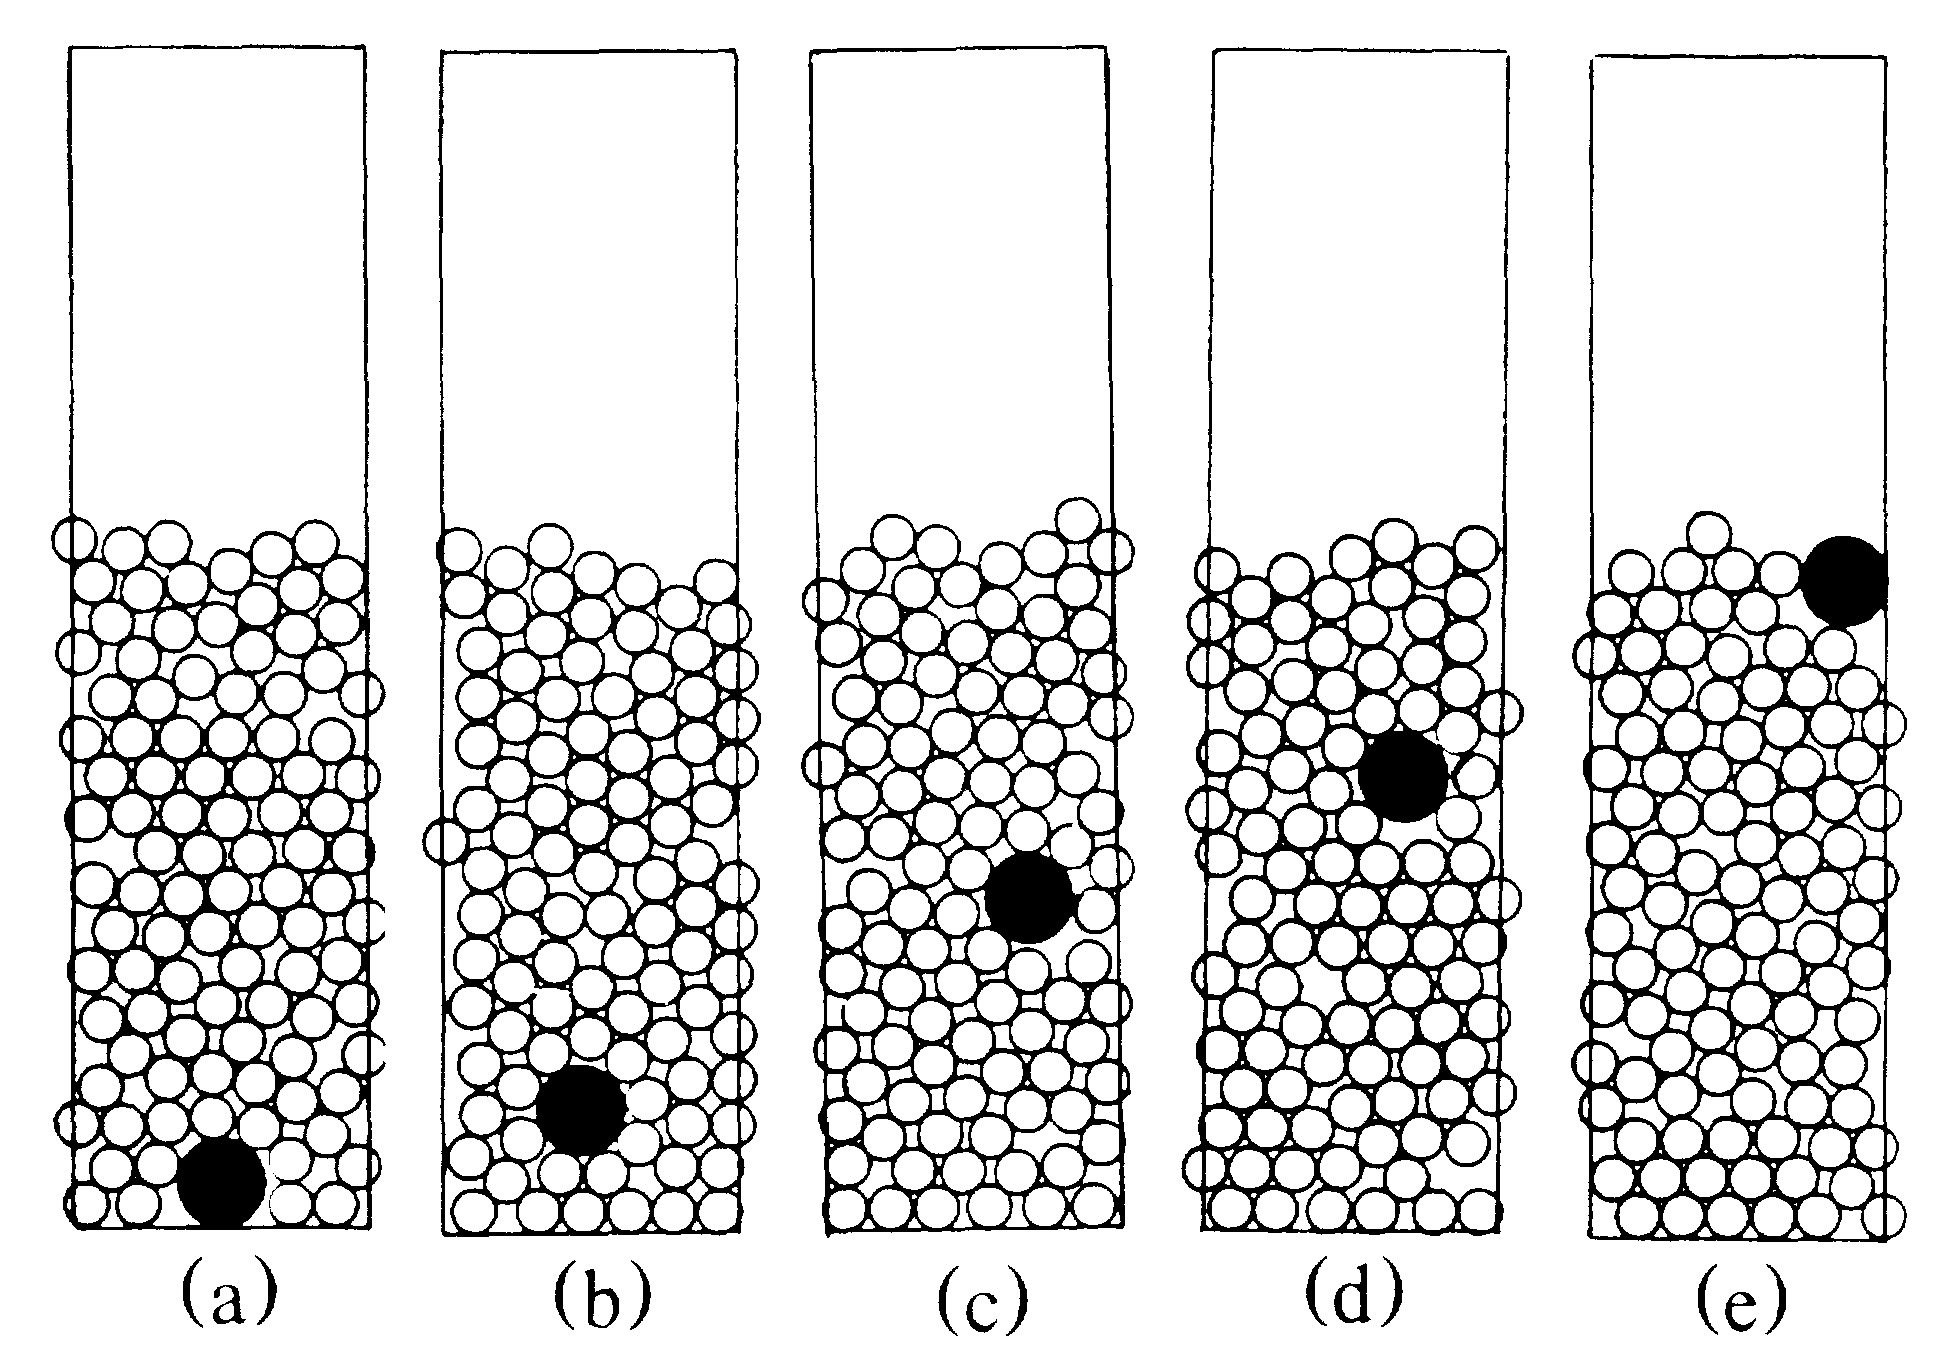
\includegraphics[width=0.65\textwidth]{04-figuras/BNE_Rosato.png}
    \caption[BNE cycles.]{Temporal evolution of shaken system of particles with periodic boundary conditions using Monte Carlo simulation. Initial configuration in Panel (a) and equally time spaced from Panels (a) to (e). Figure taken from \cite{Why_the_Brazil_nuts_are_on_top}.}
    \label{fig:BNE_rosato}
\end{figure}

%    Vários diagramas de fase foram observados para alguns dos parâmetros do BNE. Dentre as principais variáveis estão a razão de diâmetros dos grãos e a razão de densidades \cite{A_Horizontal_Brazil-Nut_Effect_and_Its_Reverse, Brazil-Nut_effect_Size_separation_of_granular_particles, Brazil-nut_effect_versus_reverse_Brazil-nut_effect_in_a_moderately_dense_granular_fluid, Categorization_of_Brazil_nut_and_its_reverse_under_less-convective_conditions_for_microgravity_geology, Competition_of_Brazil_nut_effect_buoyancy_and_inelasticity_induced_segregation_in_a_granular_mixture, Reverse_Brazil_Nut_Problem_Competition_between_Percolation_and_Condensation, Reversing_the_Brazil-Nut_Effect_Competition_between_Percolation_and_Condensation, Reverse_buoyancy_in_a_vibrated_granular_bed_Computer_Simulations, Scaling_behavior_in_convection-driven_Brazil-nut_effect, Segregation_in_a_fluidized_binary_granular_mixture_Competition_between_buoyancy_and_geometric_forces, Simple_model_for_reverse_buoyancy_in_a_vibrated_granular_system}. Dentro das caracterizações dos planos de fase, a aceleração adimensional, mostrado na equação \ref{equ:gamma}, é o parâmetro de comparação relacionado à subida do intruso.
    The most important number used in the BNE studies is the dimensionless acceleration, shown in the equation \ref{equ:gamma}. The dimensionless number is a comparison between the maximum amplitude of the vibrational acceleration and gravity. 
\begin{equation}
    \label{equ:gamma}
    \Gamma = \frac{A\omega^{2}}{g},
\end{equation}
%em que $\Gamma$ é o adimensional, $A$ é a amplitude de vibração do sistema, $\omega$ é a frequência de vibração e $g$ é o valor da gravidade.
where $\Gamma$ a dimensionless number that compares shaken acceleration with gravity, $A$ is the system amplitude of the vibration, $\omega$ is the frequency of vibration, and $g$ is the value of gravity. When $\Gamma > $ 1, then the intruder can rise, since the ascending part of the oscillation rises the magnitude of the chain forces in the media, but when the system is descending the lighter grains occupies the void space left by the bead, causing the ratchet effect. If $\Gamma < $ 1, then the intruder is not able to move, since chain forces stays there. This is the basic explanation, but not all cases work like it, as we see in some of our simulations, in Chapter \ref{chap:Resultados-BNE}.

    An experimental problem is proposed in \cite{Inertia_in_the_Brazil_nut_problem}, like we study in Chapter \ref{chap:Resultados-BNE}. In their experiment a metallic bead is placed at bottom and then agitated. They use a cylinder silo and spherical grains with size ratio between intruder and media of 3, and $\Gamma$ varies from 2.6 to 3.4, which leads the bead to rise over the media. There is a collapse of the curves involving the intruder position, the amplitude of the vibration $A$ and the oscillation period $\omega$ like in figure \ref{fig:BNE_molinari}. What we could find in our simulations is that frictionless walls also cause the bead to rise through convection currents, and the ascent ratio is similar with and without friction on the walls, see Figure \ref{fig:BNE25000_sem_Atrito_Parede}. %Refutar a tese de sem atrito nas paredes o sistema não funcionar. %Também refutar a ideia de que a ascenção do intruso não está correlacionada com as correntes de convecção. 

\begin{figure}
    \centering
    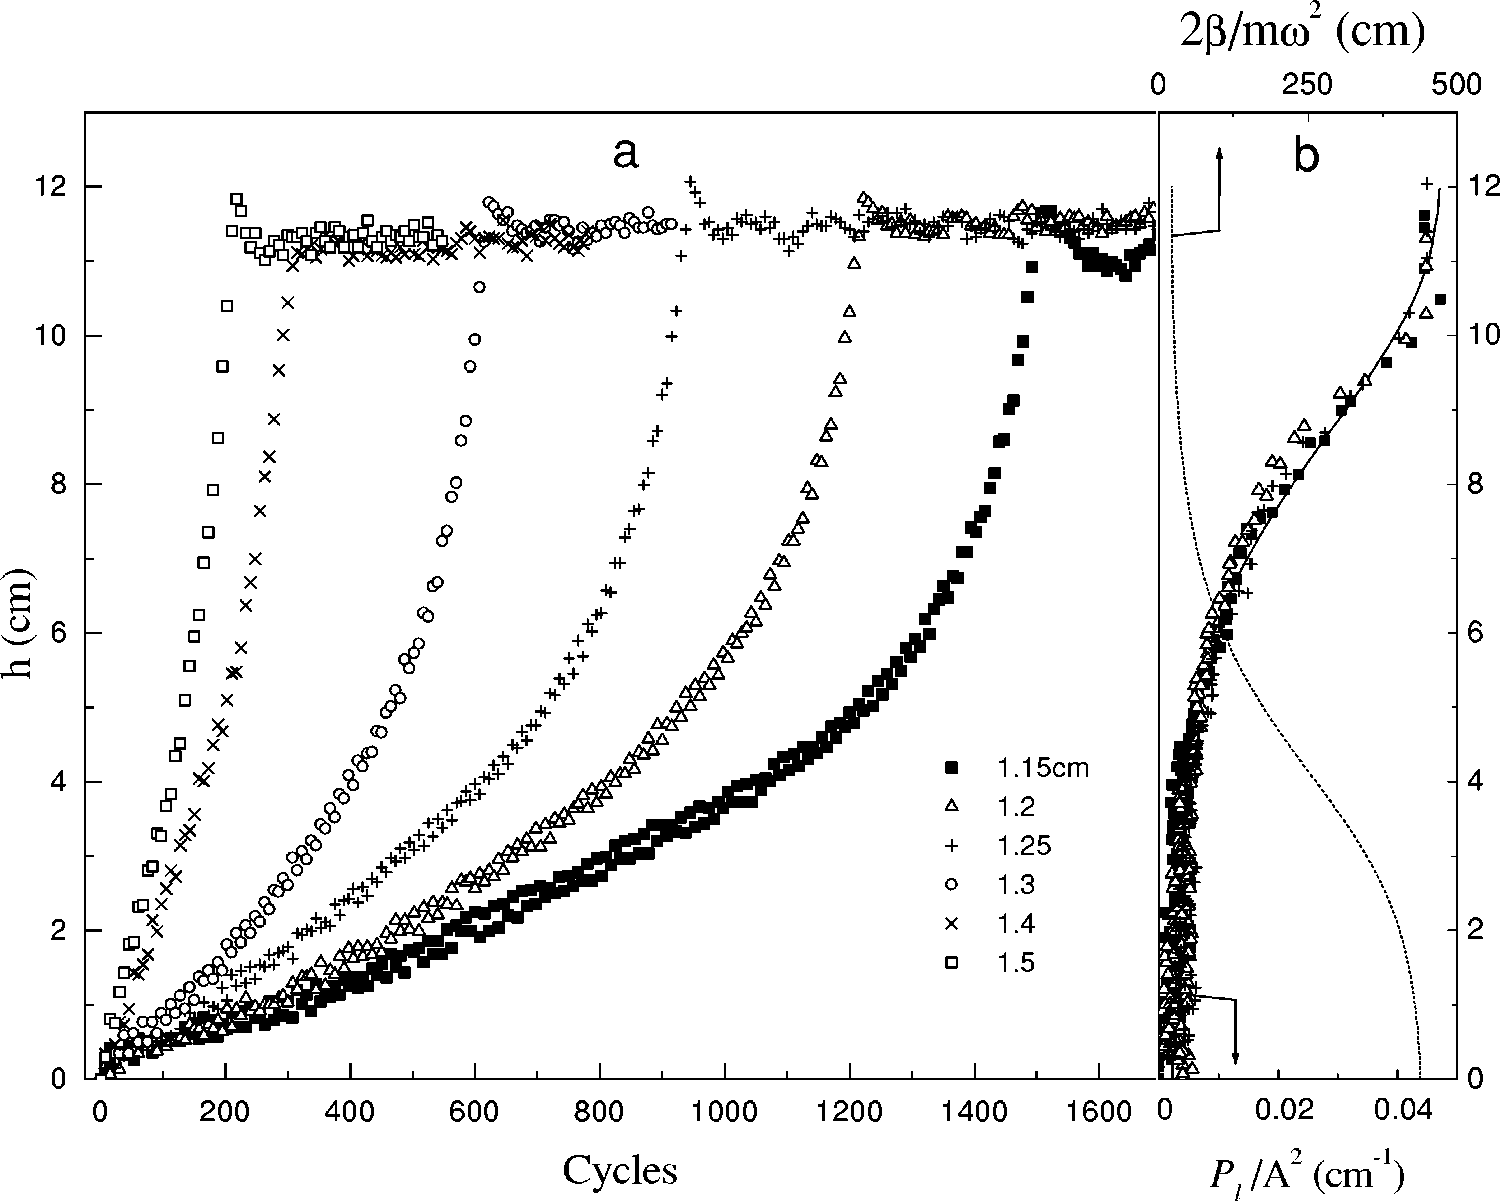
\includegraphics[width=0.65\textwidth]{04-figuras/BNE_Molinari.png}
    \caption[Intruder height in an agitated media.]{Evolution of the bead in an agitated media within a cylinder silo. Panel (a) shows the height of the intruder versus time, while Panel (b) shows the collapse of the curves. Figure taken from \cite{Inertia_in_the_Brazil_nut_problem}.}
    \label{fig:BNE_molinari}
\end{figure}

    The BNE is also influenced by the fluid that surrounds the media. In some cases, the air is relevant in the convection currents, and then leading to segregation, while vacuum leads to mixing \cite{Brazil-Nut_effect_Size_separation_of_granular_particles, Inertia_in_the_Brazil_nut_problem}. A more viscous fluid than air, like water, changes the regime of ascension of the bead, and the main mechanism that explains it is not the drag it self but the enhance of the ratcheting effect \cite{The_water-enhance_Brazil_nut_effect}.

    Several phase diagrams were observed for some of the BNE parameters. The two main variables usually analysed are the ratio of the diameters of grains and the ratio of densities of grains, as shown in Figure \ref{fig:BNE_mobius}. Another BNE phase diagram proposed by \cite{Scaling_behavior_in_convection-driven_Brazil-nut_effect} takes into account the dimensionless acceleration $\Gamma$ and the vibration threshold velocity $v_c = A \omega$.

\begin{figure}
    \centering
    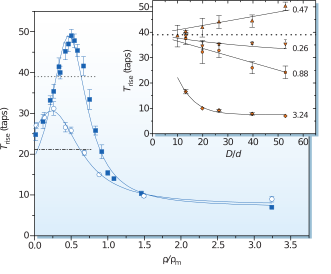
\includegraphics[width=0.65\textwidth]{04-figuras/BNE_Mobius.png}
    \caption[Phase diagram of BNE: density ratio and size ratio.]{BNE dependence on density and size ratio. The ascent time $T_{rise}$ in the main Panel versus density rate, with size ratio of 5.08 between intruder and grains with different atmospheric pressures: 1 atm. in squares ($\textcolor{blue}{\blacksquare}$) and 90 torr in circles ($\textcolor{blue}{\circ}$). The ascent time $T_{rise}$ versus the size ratio for different density ratios: 0.44, 0.48, 0.88 and 3.1. Figure taken from \cite{Brazil-Nut_effect_Size_separation_of_granular_particles}.}
    \label{fig:BNE_mobius}
\end{figure}

\begin{figure}
    \centering
    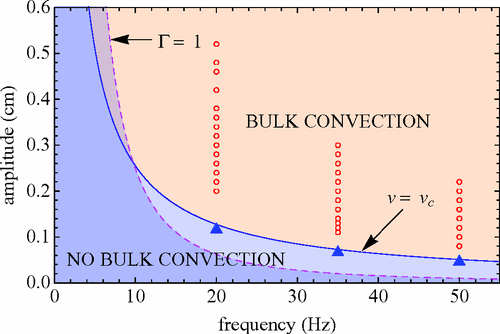
\includegraphics[width=0.65\textwidth]{04-figuras/BNE_Hejmady_PhaseSpace.png}
    \caption[Phase diagram of BNE: $\Gamma$ and $v_c$.]{BNE dependence on the dimensionless acceleration $\Gamma$ and a critical velocity $v_c$. Values of $\Gamma$ < 1 makes the intruder not rise, but also a $v < A \omega$. Figure taken from \cite{Scaling_behavior_in_convection-driven_Brazil-nut_effect}.}
    \label{fig:BNE_hejmady_convection}
\end{figure}

    Another correlated phenomena to BNE is the Reverse BNE (RBNE), in which the bead instead of rises it sinks. Many works enhanced the characterization of BNE and RBNE, in theoretical field, experimental results and numerical simulations \cite{A_Horizontal_Brazil-Nut_Effect_and_Its_Reverse, Brazil-nut_effect_versus_reverse_Brazil-nut_effect_in_a_moderately_dense_granular_fluid, Categorization_of_Brazil_nut_and_its_reverse_under_less-convective_conditions_for_microgravity_geology, Competition_of_Brazil_nut_effect_buoyancy_and_inelasticity_induced_segregation_in_a_granular_mixture, Reverse_Brazil_Nut_Problem_Competition_between_Percolation_and_Condensation, Reverse_buoyancy_in_a_vibrated_granular_bed_Computer_Simulations, Reversing_the_Brazil-Nut_Effect_Competition_between_Percolation_and_Condensation, Segregation_in_a_fluidized_binary_granular_mixture_Competition_between_buoyancy_and_geometric_forces, Simple_model_for_reverse_buoyancy_in_a_vibrated_granular_system, Hydrodynamic_theory_for_reverse_brazil_nut_segregation_and_the_non-monotonic_ascension_dynamics}. Some of these diagrams are presented here in Figures \ref{fig:RBNE_breu}, \ref{fig:RBNE_schnautz} and \ref{fig:RBNE_trujillo}.

\begin{figure}
    \centering
    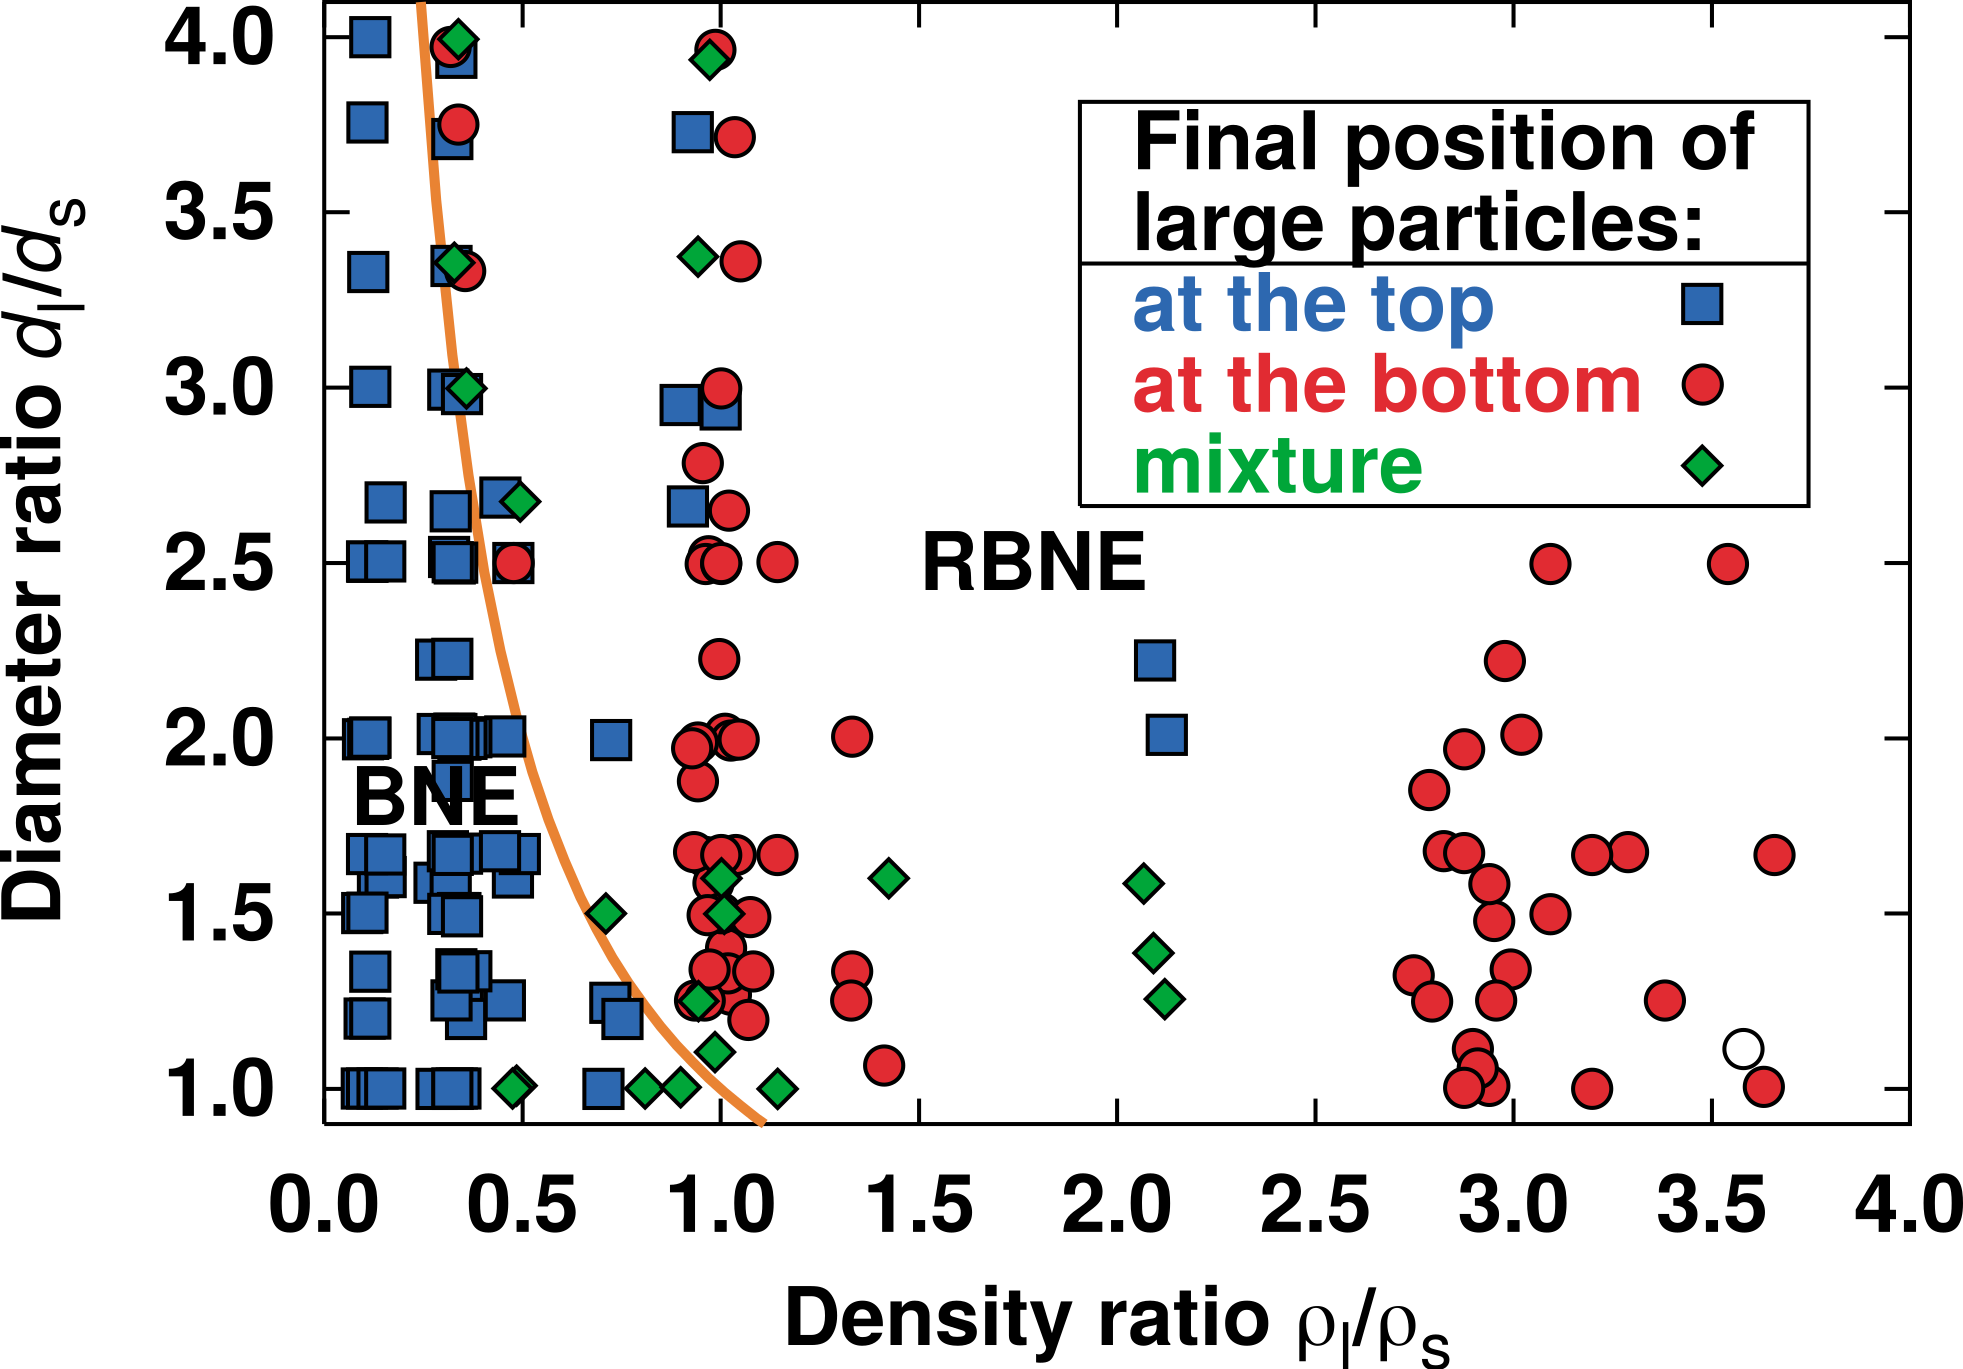
\includegraphics[width=0.65\textwidth]{04-figuras/BNE_Breu.png}
    \caption[Phase diagram of BNE/RBNE from experiment: density ratio and size ratio.]{BNE and RBNE dependence on the density ratio and the size ratio in vibrated base. The diagram shows the regime where beads rises in blue ($\textcolor{blue}{\blacksquare}$) causing the BNE, sinks in red ($\textcolor{red}{\blacksquare}$) and is mixed in green ($\textcolor{green}{\blacksquare}$). Figure taken from \cite{Reversing_the_Brazil-Nut_Effect_Competition_between_Percolation_and_Condensation}.}
    \label{fig:RBNE_breu}
\end{figure}

\begin{figure}
    \centering
    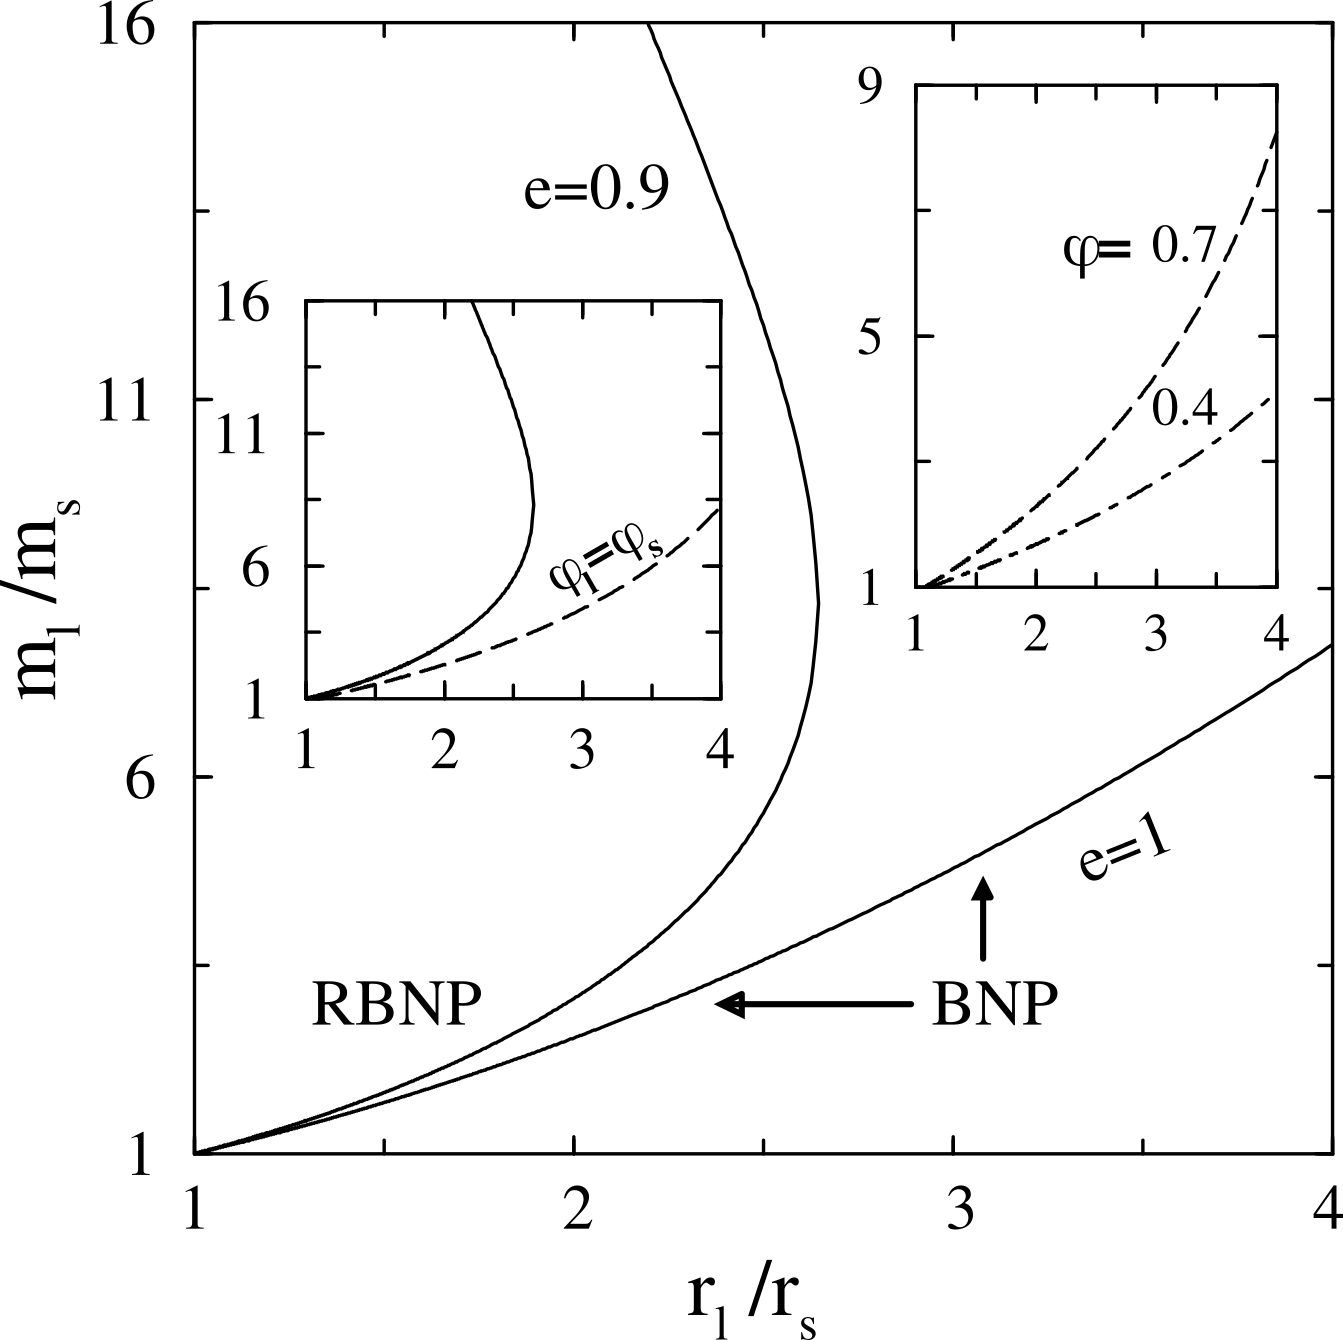
\includegraphics[width=0.65\textwidth]{04-figuras/BNE_Trujillo.png}
    \caption[Phase diagram of BNE/RBNE from analytics: density ratio and size ratio.]{BNE and RBNE dependence on the density ratio and the size ratio in vibrated base. The diagram shows the BNE-RBNE regime extracted from analytical equations of the forces in the system. $e$ is the restitution coefficient, $\phi$ is the packing fraction, $\phi_{l}$ is the portion of the packing fraction related to the intruders, $\phi_{s}$ is the packing fraction of the other grains. Left inset: phase diagram with $e$ = 0.9, $\phi_{l} / \phi_{s}$ = 10$^{-8}$ (solid curve) and $\phi_{l} / \phi_{s}$ = 1 (dashed curve). Right inset: phase diagram with $e$ = 0.9, $\phi_{l} / \phi_{s}$ = 1, $\phi$ = 0.7 (dashed curve) and $\phi$ = 0.4 (dot-dashed curve). Figure taken from \cite{Segregation_in_a_fluidized_binary_granular_mixture_Competition_between_buoyancy_and_geometric_forces}.}
    \label{fig:RBNE_trujillo}
\end{figure}

\begin{figure}
    \centering
    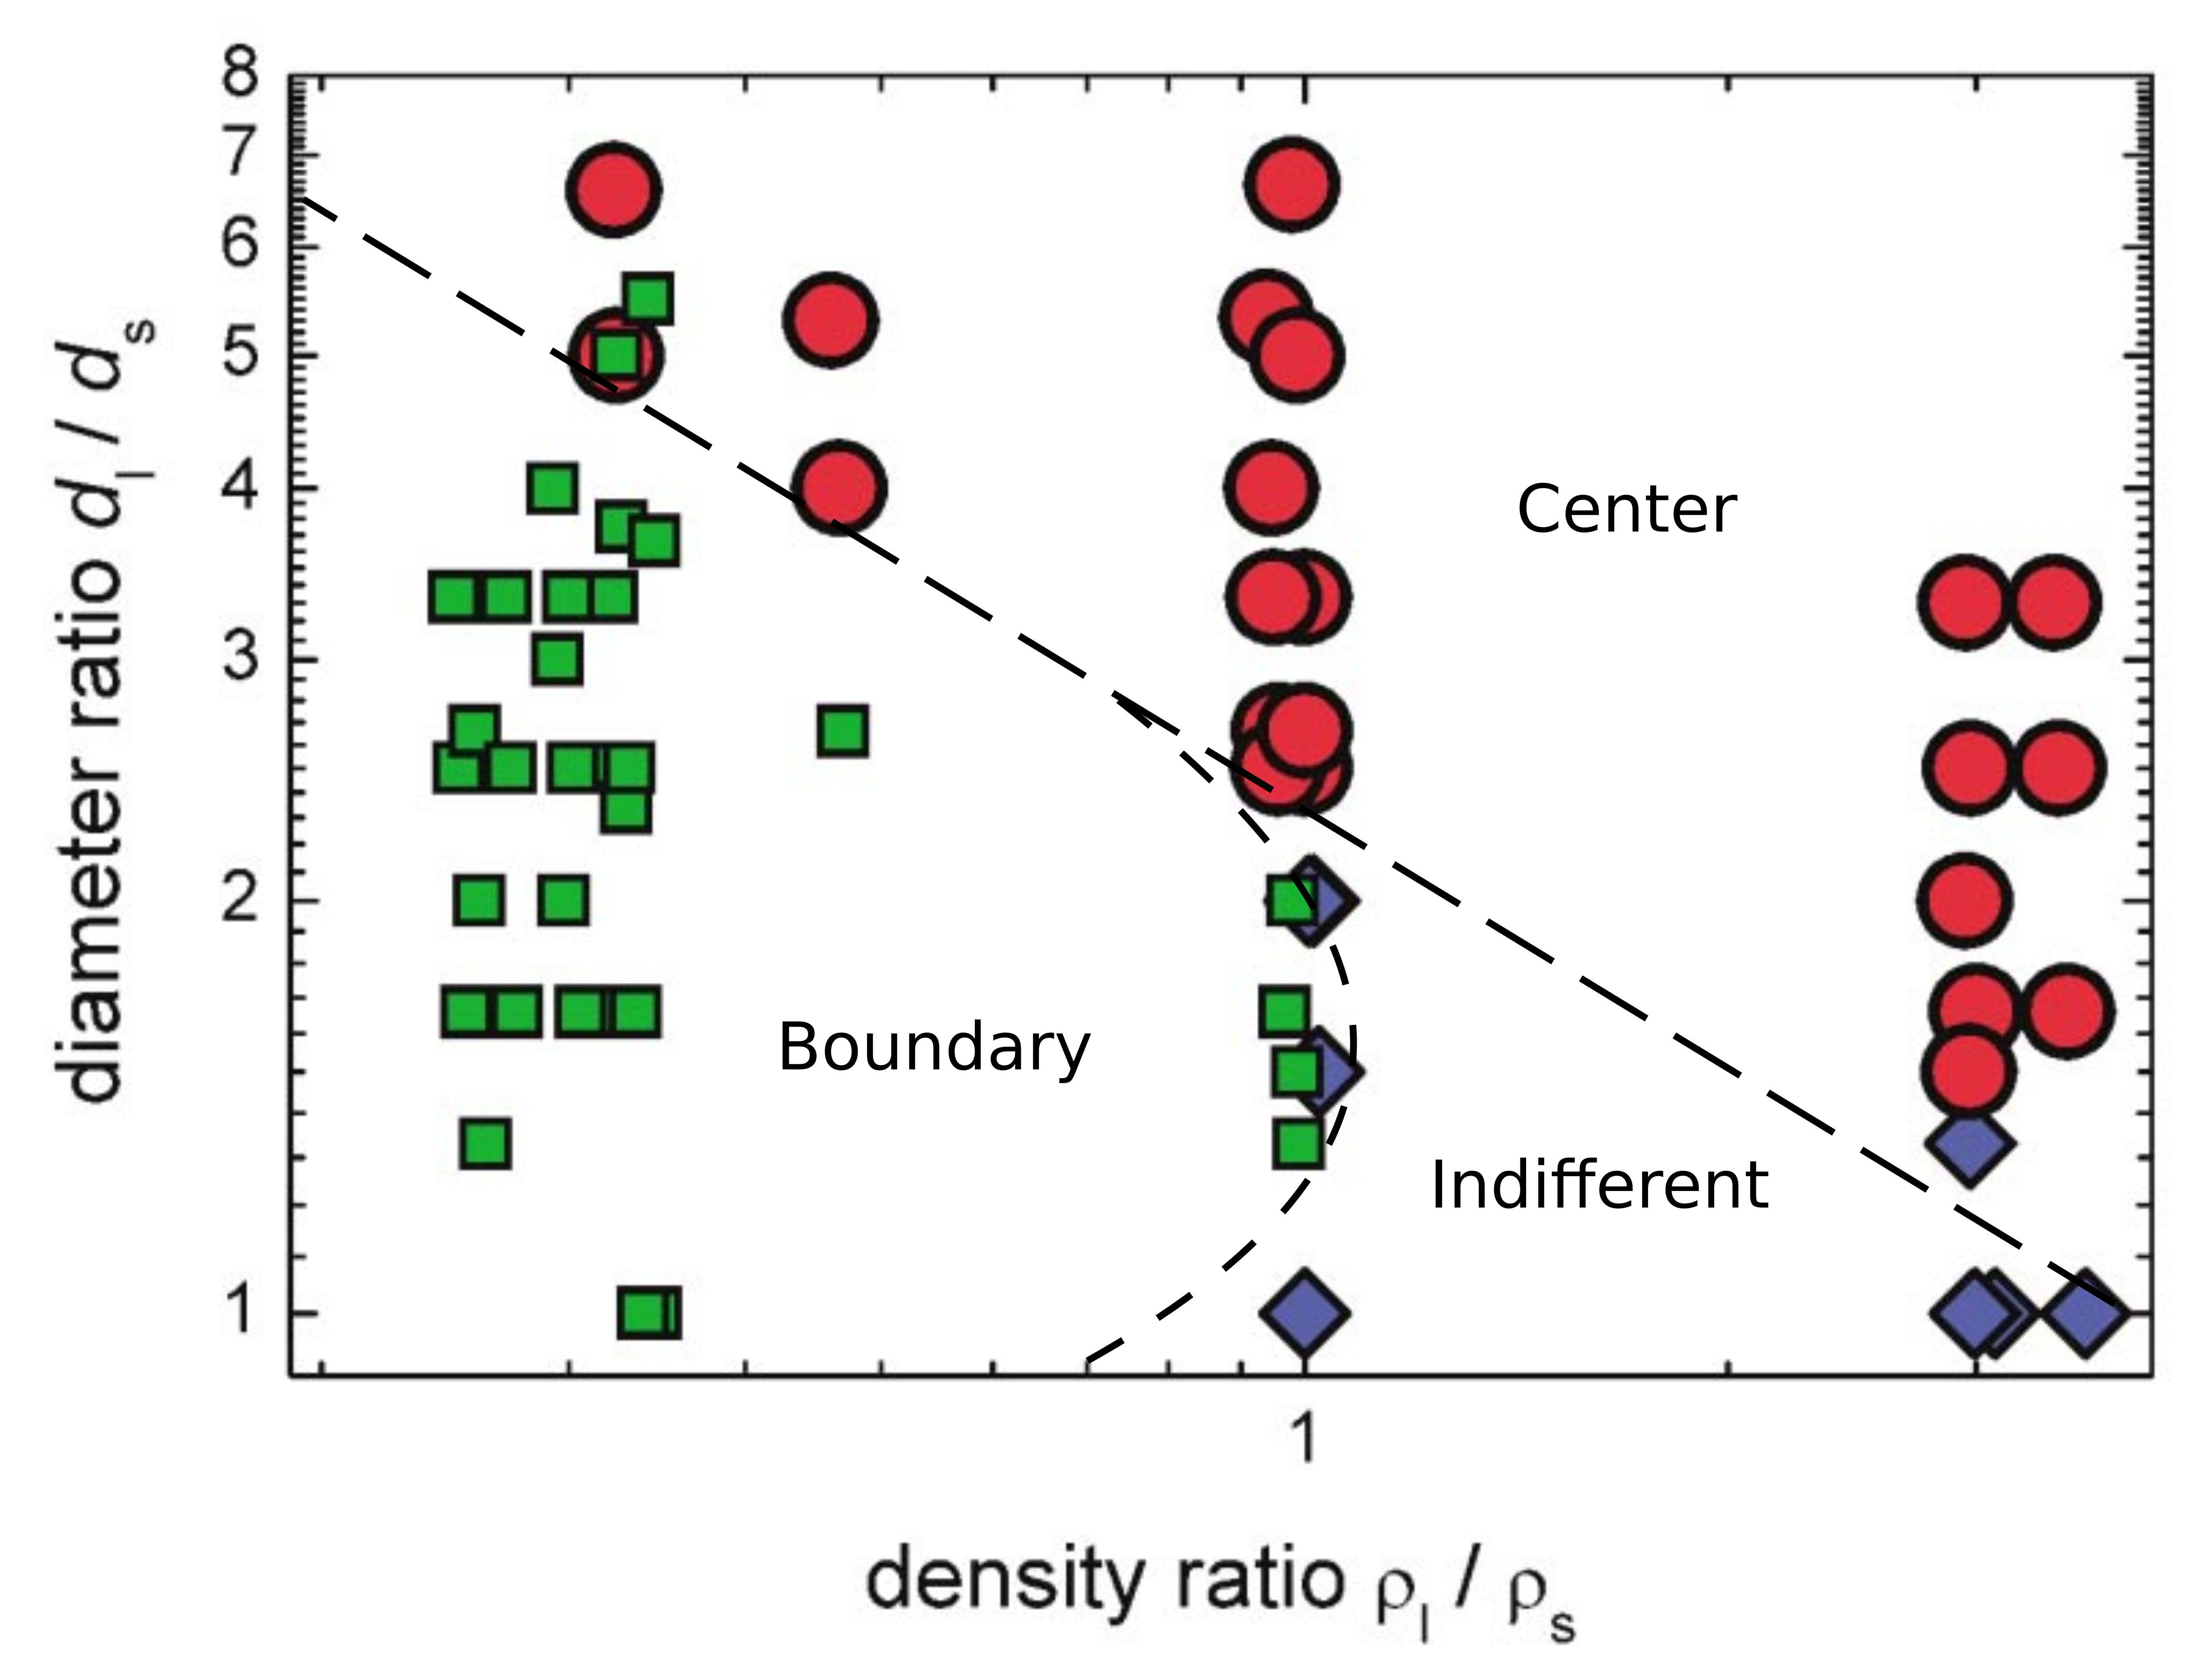
\includegraphics[width=0.65\textwidth]{04-figuras/BNE_Schnautz.png}
    \caption[Phase diagram of BNE/RBNE in swirling: density ratio and size ratio.]{BNE and RBNE dependence on the density ratio and the size ratio in swirling base. The diagram shows the regime where beads segregates in red ($\textcolor{red}{\CIRCLE}$), aggregates in green ($\textcolor{green}{\blacksquare}$) and is indifferent in blue ($\textcolor{blue}{\Diamondblack}$). Figure taken from \cite{A_Horizontal_Brazil-Nut_Effect_and_Its_Reverse}.}
    \label{fig:RBNE_schnautz}
\end{figure}

    Recently the Reference \cite{Size_segregation_of_irregular_granular_materials_captured_by_time-resolved_3D_imaging} experimentally shows that in a mixture of irregular ellipsoidal shape firstly reorient vertically, but without changing significantly their height; secondly, the grains rise upwards, and while doing so, they still tend to stay vertically aligned; and finally, when the grains reach the top, they tend to realign horizontally on the surface.

    If the intruder of the media has a non uniform distribution geometry, like a polar particle, inserted in a layer of circular grains, and when the media is agitated, the intruder starts to "self-propel" at the direction it is oriented \cite{Symmetry_properties_of_the_large-deviation_function_of_the_velocity_of_a_self-propelled_polar_particle}. This is another property that non uniform shaken granular exhibit, reorienting the position or "propelling-itself".

    %Referência do intruso andando no meio granular (está no artigo e inspirou o uso do LDF).

%Reverse BNE: A_Horizontal_Brazil-Nut_Effect_and_Its_Reverse, Brazil-nut_effect_versus_reverse_Brazil-nut_effect_in_a_moderately_dense_granular_fluid, Caracterization_of_Brazil_nut_and_its_reverse_under_less-convective_conditions_for_microgravity_geology, Competition_of_Brazil_nut_effect_buoyancy_and_inelasticity_induced_segregation_in_a_granular_mixture, Reverse_Brazil_Nut_Problem_Competition_between_Percolation_and_Condensation, Reverse_buoyancy_in_a_vibrated_granular_bed_Computer_Simulations, Reversing_the_Brazil-Nut_Effect_Competition_between_Percolation_and_Condensation, Segregation_in_a_fluidized_binary_granular_mixture_Competition_between_buoyancy_and_geometric_forces, Simple_model_for_reverse_buoyancy_in_a_vibrated_granular_system, Hydrodynamic theory for reverse brazil nut segregation and the non-monotonic ascension dynamics
%Vibrações verticais: Inertia_in_the_Brazil_nut_problem, The_water-enhance_Brazil_nut_effect, Brazil-Nut_effect_Size_separation_of_granular_particles, Caracterization_of_Brazil_nut_and_its_reverse_under_less-convective_conditions_for_microgravity_geology, Competition_of_Brazil_nut_effect_buoyancy_and_inelasticity_induced_segregation_in_a_granular_mixture, Reverse_buoyancy_in_a_vibrated_granular_bed_Computer_Simulations, Reversing_the_Brazil-Nut_Effect_Competition_between_Percolation_and_Condensation, Scaling_behavior_in_convection-driven_Brazil-nut_effect
%Vibrações laterais: Size_segregation_of_irregular_granular_materials_captured_by_time-resolved_3D_imaging, A_Horizontal_Brazil-Nut_Effect_and_Its_Reverse, 

%    No próximo capítulo, descreveremos os resultados obtidos ao simularmos o BNE.
    Next Chapter, we describe the results of our BNE simulations using the techniques presented in Chapter \ref{chap:DEM}.

%    Inertia_in_the_Brazil_nut_problem -> Atribui a convecção ao atrito das paredes e colapsa as curvas de ascensão.
%    The_water-enhance_Brazil_nut_effect -> Uso do fluido intersticial com BNE.
%    Why_the_Brazil_Nuts_are_on_top -> Atribui o BNE ao efeito catraca, usando Monte Carlo e desprezando atrito e a massa é desprezível para o efeito.
%    A_Horizontal_Brazil-Nut_Effect_and_Its_Reverse -> Vibra horizontalmente e com diferentes materiais (densidades), reproduz BNE (ida para o centro) e rBNE (ida para as bordas). Frequências de 0.5 à 2Hz, amplitude de $3,175n$mm, com $n$ variando de $3 ... 7$, diâmetro médio dos grãos de 6mm, diâmetro do intruso $1,3 ... 7$ vezes o diâmetro dos grãos e coeficiente de atrito de $0,67$. Exibe um diagrama de fase Diâmetro/Densidade.
%    Brazil-Nut_effect_Size_separation_of_granular_particles -> Descreve o fenômeno em função do diâmetro e da densidade, fixa a frequência em $13$Hz e a amplitude em $7,35$mm e o diâmetro do grão menor em $0,5$mm, ou seja, a relação amplitude e diâmetro do grão é de $14,7$ vezes. Diâmetro do intruso pode chegar à $25,4$mm, o equivalente $50800$ vezes o diâmetro do grão.
%    Brazil-nut_effect_versus_reverse_Brazil-nut_effect_in_a_moderately_dense_granular_fluid -> Analítico/teórico sobre os planos de fase das regiões BNE e rBNE em função do diagrama Diâmetro/Densidade com coeficiente de compactação e restituição.
%    Caracterization_of_Brazil_nut_and_its_reverse_under_less-convective_conditions_for_microgravity_geology -> Reproduz o BNE em condição fechada, porém com atrito baixo entre parede/grão, com condições de aceleração menores q a gravidade.
%    Competition_of_Brazil_nut_effect_buoyancy_and_inelasticity_induced_segregation_in_a_granular_mixture -> Compara os resultados do BNE em função das massas, diâmetros e coeficientes de restituição.
%    Reverse_Brazil_Nut_Problem_Competition_between_Percolation_and_Condensation -> Mostra o diagrama qualitativo da transição BNE para rBNE em função da razão dos diâmetros pelas massas. Relaciona a temperatura granular.
%    Reverse_buoyancy_in_a_vibrated_granular_bed_Computer_Simulations -> Insere um fluido como amortizador e demonstra as forças e seus efeitos.
%    Reversing_the_Brazil-Nut_Effect_Competition_between_Percolation_and_Condensation -> Mostra o diagrama BNE/rBNE em função da densidade versus diâmetro, com o diagrama de frequência por aceleração normalizada.
%    Scaling_behavior_in_convection-driven_Brazil-nut_effect ->  mostra o esquema de convecção para a contribuição no BNE
%    Segregation_in_a_fluidized_binary_granular_mixture_Competition_between_buoyancy_and_geometric_forces -> Diagrama BNE/rBNE densidade versus diâmetro
%    Simple_model_for_reverse_buoyancy_in_a_vibrated_granular_system -> Velocidade no BNE/rBNE densidade
%    Study_the_effect_of_vibration_frequency_and_amplitude_on_the_quality_of_fluidization_of_a_vibrated_granular_flow_using_discrete_element_method -> Caracteriza o fluido em função da altura do sistema.

%    Size_separation_in_vibrated_granular_matter -> Compilado dos artigos acima

%    Convection_Cells_in_Vibrating_Granular_Media -> Em relação ao BNE não é mostrado, uma vez q a distribuição dos raios dos grãos são próximas entre si. Mostra a convecção na agitação dos granulares, mesmo quando possuem condição periódica de contorno. Porém a agitação é muito alta.
 % Fundamentação teórica - BNE
% -----------------------------------------------------------------------------
% Resultados
% -----------------------------------------------------------------------------

\chapter{Result Analysis and Discussion - BNE}
\label{chap:Resultados-BNE}

%Cada capítulo deve conter uma pequena introdução (tipicamente, um ou dois parágrafos), em seção não numerada, que deve deixar claro o objetivo e o que será discutido no capítulo, bem como a organização do capítulo.

%\section{Título da seção}
%\label{sec:titSecResult}

%Inserir seu texto aqui...

%    Nesta parte da tese, utilizaremos 2500 grãos. O diâmetro médio do grão é $d = 1\pm 2.5\%$, distribuídos uniformemente. O diâmetro do intruso é de $D = 5$ vezes o diâmetro médio dos grãos. A densidade de todos os grãos é a mesma, e vale $\rho = 1/\pi$, e portanto a massa média dos grãos é de $m = 0,25$, exceto quando estiver ressaltado nas figuras. A constante de mola na direção normal é de $k_{n} = 1000$ e a tangencial é de $k_{t} = 750$. A atuação do amortecedor é no regime crítico ($\gamma = 2\sqrt{m k}$), e vale aproximadamente $\gamma = \sqrt{10}$. O atrito dos grãos valem $\mu = 0,5$, tanto entre grãos, quanto entre paredes, quando houver. O passo de tempo ($dt=pT$) vale aproximadamente $dt = \frac{1}{2000\sqrt{10}}$, utilizando a fração de $p=0,01$ do período de oscilação do modelo de contato massa mola $T = \sqrt{\frac{m}{k}}$. A largura da caixa é de $L = 37.5$ diâmetros de grão.

    In this Chapter we will present the results obtained from BNE simulations. These results were published in Reference \cite{Large-deviation_quantification_of_boundary_conditions_on_the_Brazil_nut_effect}, also present in Appendix \ref{appendix:BNE}. The parameters we used to simulate the system is 2500 grains, with average diameter $d$ = 1 $\pm$ 2.5\%, with uniform distribution, the intruder diameter $D$ = 5$d$. Grains and intruder density $\rho$ = 4/$\pi$, leading the average mass $m$ = 1, the spring constant in the normal direction $k_{n}$ = 1000 and the spring constant in the tangential direction $k_{t}$ = 750, the critical damping coefficient $\gamma$ = 2$\sqrt{m_r k_{n}}$, $m_r$ = $\frac{m_i m_j}{m_i + m_j}$, the friction coefficient $\mu$ = 0.5 between grain-grain contact, grain-intruder contact, grain-wall intruder contact and intruder-wall contact. The time step dt = $\frac{1}{100}\sqrt{\frac{m_r}{k_n}}$, the width $w$ = 37.5$d$, the gravity acceleration $g$ = 1. Any different parameter used is described properly in each corresponding Figure and in the text. As an example, Figure \ref{fig:BNE}.

%    Inicialmente, estudamos o sistema com paredes no fundo e nas laterais, formando uma caixa. Observamos, nestas simulações, correntes de convecção próximas às paredes.

\begin{figure}
    \centering
    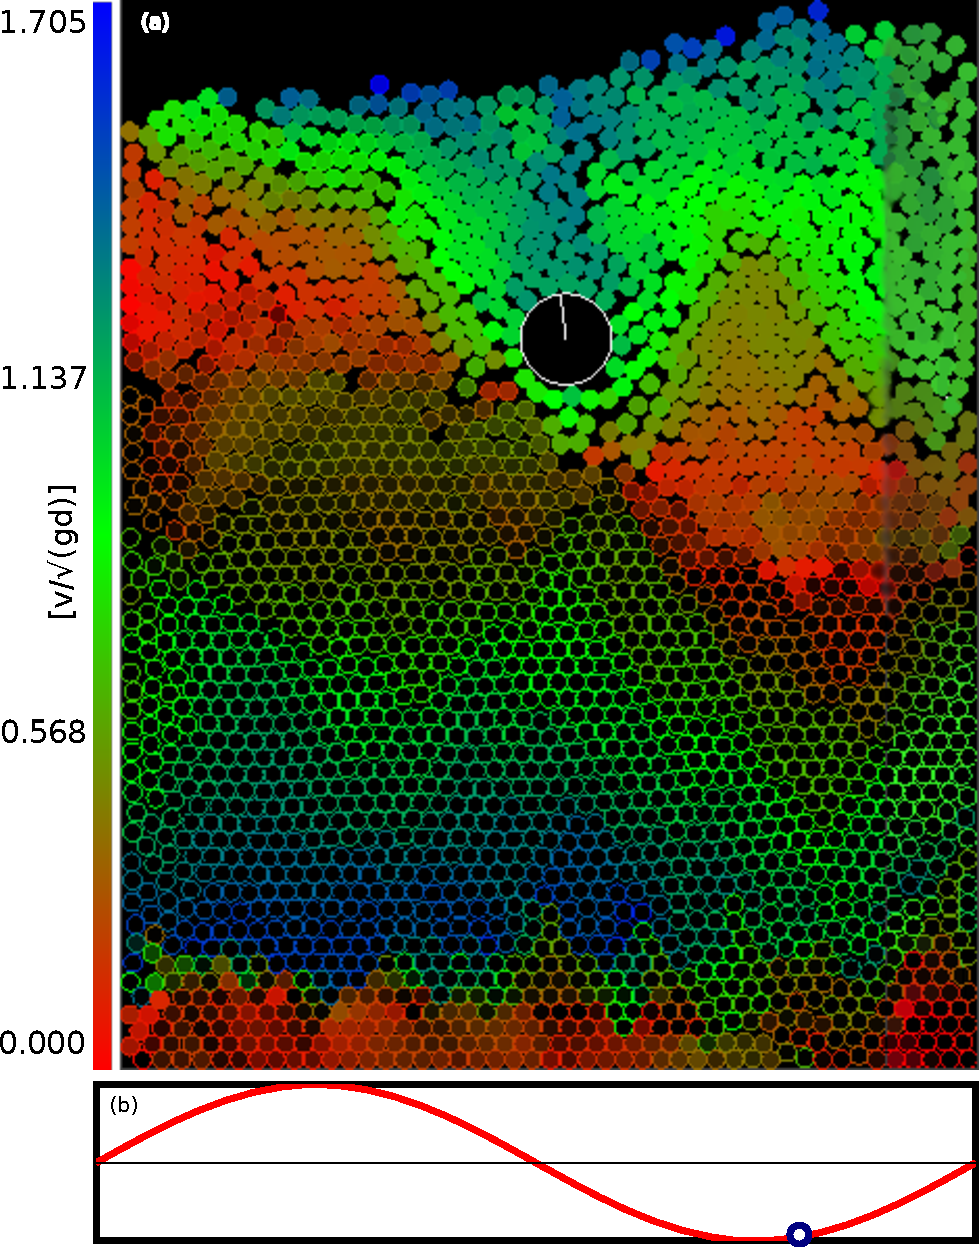
\includegraphics[width=0.65\textwidth]{04-figuras/BNE.pdf}
    \caption[BNE snapshot.]{In panel (a), a snapshot of the system lateral walls. Grains are represented by discs: hollow discs ($\textcolor{black}{\circ}$) are moving downward (with gravity) while filled ones ($\textcolor{black}{\bullet}$) are moving upward (against gravity). Color level shown at left side indicates the magnitude of the speed: red indicates no movement while blue indicates the maximum value for the speed. It is worth noting the inertia of the intruder accelerating the grains above him (bluish grains). It is also possible to observe the transition between the grains rising and falling in the reddish region around the intruder, a characteristic responsible for the granular ratchet effect. While the intruder easily displaces the grains on the way up, he is unable to move the grains that descend due to the steric exclusion. In panel (b) a sinusoidal displacement imposed to the substrate. This snapshot was taken after the minimum of the oscillation of the substrate, marked as a blue dot in this plot. Figure also present in \cite{Large-deviation_quantification_of_boundary_conditions_on_the_Brazil_nut_effect}.}
    \label{fig:BNE}
\end{figure}

    Initially, we studied the system with bottom and sidewalls, forming a box. In these simulations, we observed convection currents close to the walls. This convection currents are the main contribution to the rise of the intruder. The sequential position of the intruder in a single example is shown in Figure \ref{fig:BNE_intruderwalls}.

\begin{figure}
    \centering
    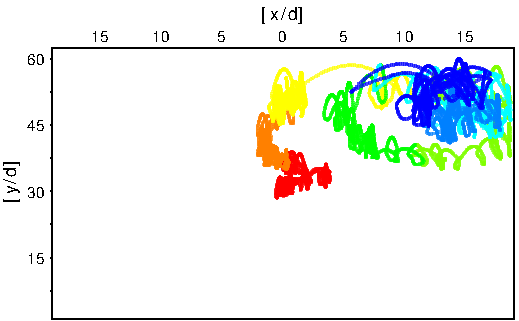
\includegraphics[width=0.65\textwidth]{04-figuras/BNE_PositionWalls.pdf}
    \caption[BNE with walls: sample of intruder positions.]{Sequential positions of the intruder $(x, y)$ taken at constant time intervals (0.316 $\sqrt{d/g}$), for a system with lateral frictional walls (fw). The shaken frequency $\omega$ = 0.256$\sqrt{d/g}$. $y$ = 0 indicates the box floor and the unities are in unities of the mean grain diameter. The change in colors indicates the time elapsed in the simulation, the red corresponds to the beginning of the simulation and the blue to the end.}
    \label{fig:BNE_intruderwalls}
\end{figure}

    The following Figures \ref{} show ascent profiles of the intruder.

\begin{figure}
    \centering
    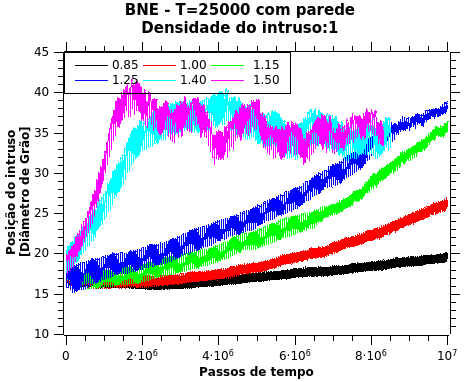
\includegraphics[width=0.65\textwidth]{04-figuras/BNE25000D1.png}
    \caption[BNE with frictional walls: $\rho_I/\rho_g$ = 1.]{Time series for intruder horizontal position at different $\Gamma$ for system with frictional walls (fw). The density $\rho_I/\rho_g$ = 1, with $\rho_I$ the density of the intruder and $\rho_g$ the density of the media. Simulations run until $...\sqrt{d/g}$. Figure also present in \cite{Large-deviation_quantification_of_boundary_conditions_on_the_Brazil_nut_effect}.}
    \label{fig:BNE25000_Parede}
\end{figure}

\begin{figure}
    \centering
    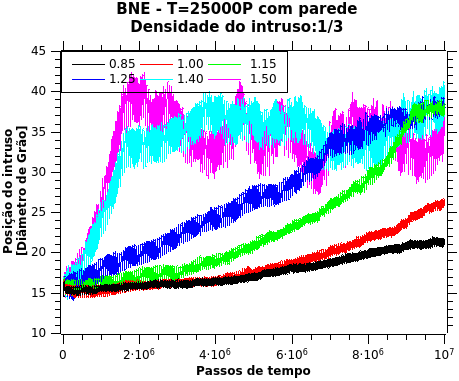
\includegraphics[width=0.65\textwidth]{04-figuras/BNE25000D1-3.png}
    \caption[BNE with frictional walls: $\rho_I/\rho_g$ = 1/3.]{Time series for intruder horizontal position at different $\Gamma$ for system with frictional walls (fw). The density $\rho_I/\rho_g$ = 1/3, with $\rho_I$ the density of the intruder and $\rho_g$ the density of the media. Simulations run until $...\sqrt{d/g}$.}
    \label{fig:BNE25000_Parede_Densidade1-3}
\end{figure}

\begin{figure}
    \centering
    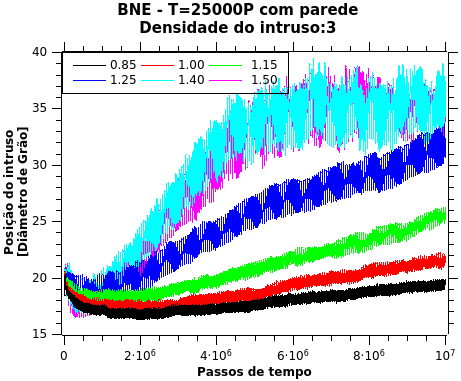
\includegraphics[width=0.65\textwidth]{04-figuras/BNE25000D3.png}
    [BNE with frictional walls: $\rho_I/\rho_g$ = 1.]{Time series for intruder horizontal position at different $\Gamma$ for system with frictional walls (fw). The density $\rho_I/\rho_g$ = 3, with $\rho_I$ the density of the intruder and $\rho_g$ the density of the media. Simulations run until $...\sqrt{d/g}$.}
    \label{fig:BNE25000_Parede_Densidade3}
\end{figure}

%    Percebemos que intrusos mais densos sobem mais lentamente que intrusos menos densos. Os tempos de subida, quando comparados, podem ser ordenados das figuras $\ref{fig:BNE25000_Parede_Densidade1-3} < \ref{fig:BNE25000_Parede} < \ref{fig:BNE25000_Parede_Densidade3}$. Assim como as correntes de convecção são mais intensas, o intruso sobe mais rapidamente e cai mais rapidamente, visto na amplitude de $\Gamma = 1,5$ para as figuras \ref{fig:BNE25000_Parede_Densidade1-3}, \ref{fig:BNE25000_Parede} e \ref{fig:BNE25000_Parede_Densidade3}, respectivamente.

    We saw that denser intruders rise more slowly than less dense intruders for all $\Gamma$. For this frequency, we saw the contrary predicted in the BNE, the denser would rise faster than the less dense. This effect may be a peculiar behavior for this frequency, or the density range we test. We also notice that the convection current is stronger the less dense the intruder is. As expected, the higher the $\Gamma$ the faster the ascent rate.

%    Quando retirado o atrito entre os grãos e as paredes, temos que o efeito da convecção no sistema diminui, ocasionando uma subida mais lenta que quando o atrito está presente. A figura \ref{fig:BNE25000_sem_Atrito_Parede} mostra a subida do intruso no sistema em que as paredes não possuem atrito.

    When frictionless walls (flw) are in play, we saw that convection decreases, causing a slower ascent rate, compared to fw. Figure \ref{fig:BNE2500_sem_Atrito_Parede} shows the intruder rise in a flw system, in opposition to the explanation in the Reference \cite{Inertia_in_the_Brazil_nut_problem}. For flw, we saw that $\Gamma$ = 0.85 was not able to rise, while fw rises with slow ascent rate.

\begin{figure}
    \centering
    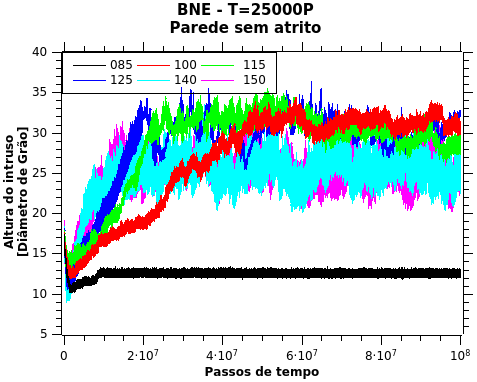
\includegraphics[width=0.65\textwidth]{04-figuras/BNE25000PsemAtrito.png}
    \caption[BNE with frictionless walls.]{Time series for intruder horizontal position at different $\Gamma$ for system with flw. The density $\rho_I/\rho_g$ = 1, with $\rho_I$ the density of the intruder and $\rho_g$ the density of the media.}
    \label{fig:BNE25000_sem_Atrito_Parede}
\end{figure}

%    Ao comparar os tempos de subida do sistema que possui atrito nas paredes (figura \ref{fig:BNE25000_Parede}) com o sistema que não possui atrito nas paredes (figura \ref{fig:BNE25000_sem_Atrito_Parede}), percebemos que o tempo de subida é maior, além de que o sistema que possui agitação menor que a gravidade não sobe, mostrando que um dos fatores que importam para o \textit{BNE} são as correntes de convecção formadas próximas das paredes.

    When comparing the rise times of fw (figure \ref{fig:BNE25000_Wall}) with flw (figure \ref{fig:BNE25000_without_Atrito_Wall}), we notice that the rise time is larger, and the system that has less agitation than gravity does not rise, showing that one of the factors that matter for the BNE are the convection currents formed close to the walls and the convection currents are enhanced by fw.

    We define the ascent rate as the difference between the initial position of the intruder to its highest position, then divide this difference by the time it takes to rise. Than we plot the ascent rate versus shaken frequency for each $\Gamma$.

\begin{figure}
    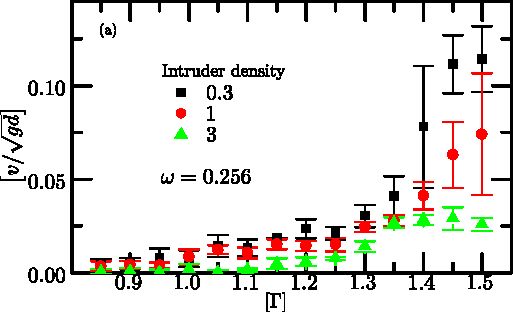
\includegraphics[width=0.65\linewidth]{04-figuras/BNE_FW_Density.pdf}
    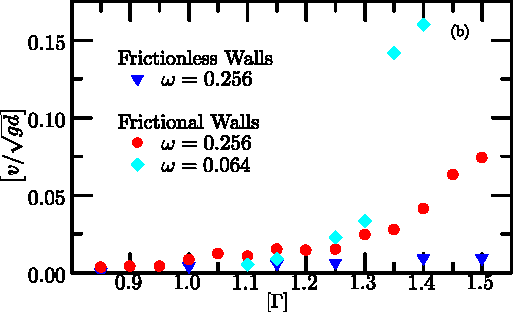
\includegraphics[width=0.65\linewidth]{04-figuras/BNE_W.pdf}
    \caption{In (a), the simulation was set to fw, width of 37.5d, shaken frequency of $0.256\sqrt{g/d}$, 2500 grains, and we have varied the intruder density, compared to the medium. In (b), a comparison between fw and flw and a change in frequency. Figure also present in \cite{Large-deviation_quantification_of_boundary_conditions_on_the_Brazil_nut_effect}.}
    \label{fig:BNE_walls}
\end{figure}

%    Quando retiramos o atrito do sistema, o intruso chega ao fundo do sistema, independente da amplitude de vibração. A figura \ref{fig:BNE25000_sem_Atrito} exibe o comportamento do intruso para o sistema sem atrito.

    When no friction is present on the system, the intruder sinks to the bottom, independently from the amplitude of the vibration. Figure \ref{fig:BNE25000_sem_Atrito} exhibits the height of the intruder in frictionless system. As expected, no friction on the system causes no BNE, and the simulations we have performed shows that the intruder sinks to bottom. We are not going to count this fact as a RBNE, since only friction has changed.

\begin{figure}
    \centering
    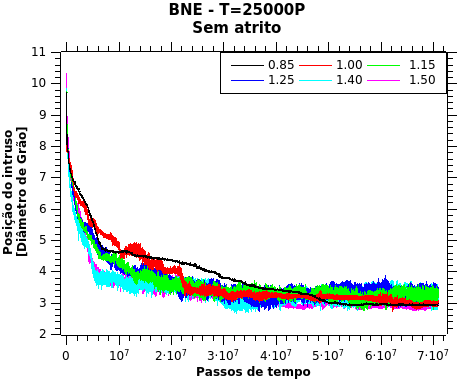
\includegraphics[width=0.65\textwidth]{04-figuras/BNE25000semAtrito.png}
    \caption[Frictionless grains and walls.]{Time series for the intruder's fall in no friction system. Independent of $\Gamma$, the intruder sinks to the bottom.}
    \label{fig:BNE25000_sem_Atrito}
\end{figure}

    If instead of having sidewalls, we replace them with a periodic boundary condition (pbc), we could have the intruder crossing from one side to another, something impossible to do with walls, but also we expect to do not have the sidewalls effect, like convection currents. As an example of the intruder position through time, Figure \ref{fig:BNE_intruderpbc}. A difference between fw and pbc is the fact that the intruder can follow the convection current in fw and sink a little bit, while in pbc it does not sink in the media.

\begin{figure}
    \centering
    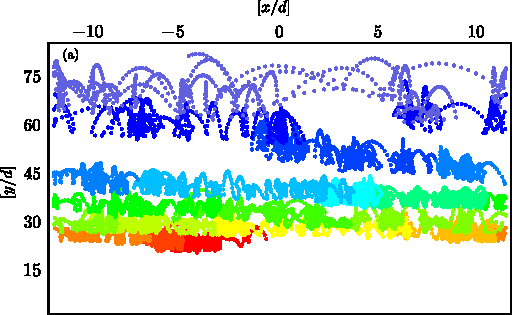
\includegraphics[width=0.65\textwidth]{04-figuras/BNE_PositionPBC.pdf}
    \caption[BNE with periodic boundary: sample of intruder positions.]{Sequential positions of the intruder $(x, y)$ taken at constant time intervals (0.316 $\sqrt{d/g}$), for a system with pbc. The shaken frequency $\omega$ = 0.213$\sqrt{d/g}$. $y$ = 0 indicates the box floor and the unities are in unities of the mean grain diameter. The change in colors indicates the time elapsed in the simulation, the red corresponds to the beginning of the simulation and the blue to the end. The width of the pbc in this sequential positions is $w$ = 25$d$. Figure also present in \cite{Large-deviation_quantification_of_boundary_conditions_on_the_Brazil_nut_effect}.}
    \label{fig:BNE_intruderwalls}
\end{figure}

%    Se ao invés de retirarmos o atrito, retirarmos as paredes laterais formando uma condição periódica de contorno de largura $28$ diâmetros de grão, verificaremos que o \textit{BNE} não acontece para o período de vibração de $25000$ passos de tempo, como mostrado na figura \ref{fig:BNE25000_Contorno}.

    The as an example of pbc intruder ascent temporal profile, Figure \ref{fig:BNE30000_Contorno}. Two differences are present here, if we compare fw and pbc: the ascent time of the intruder for each $\Gamma$ and the shaken frequency. At the same frequency applied to the fw, the pbc did not rise at all. The response is shown in Figure \ref{fig:BNE_resonance}.

%    Já no caso de períodos maiores, o BNE ocorre. A figura \ref{fig:BNE30000_Contorno} exemplifica o \textit{BNE} ocorrendo com condição periódica de contorno e período de vibração de $30000$ passos de tempo.

\begin{figure}
    \centering
    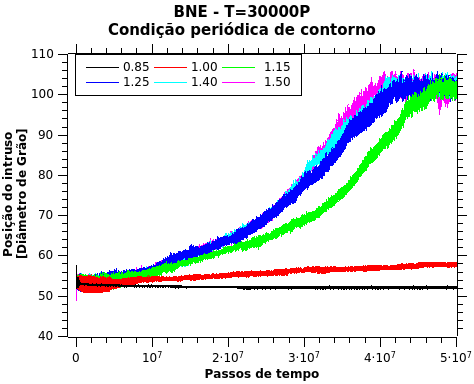
\includegraphics[width=0.65\textwidth]{04-figuras/BNE30000Contorno.png}
    \caption[BNE with periodic boundary: time series.]{Time series for intruder horizontal position at different $\Gamma$ for system with pbc. The density $\rho_I/\rho_g$ = 1, with $\rho_I$ the density of the intruder and $\rho_g$ the density of the media. The value of $\omega$ = 0.213. Figure also present in \cite{Large-deviation_quantification_of_boundary_conditions_on_the_Brazil_nut_effect}.}
    \label{fig:BNE30000_Contorno}
\end{figure}

%    Na figura \ref{fig:BNE30000_Contorno}, percebemos que acelerações menores que a gravidade não fazem o intruso ascender, enquanto acelerações próximas da gravidade tem um movimento de ascensão lento e em saltos. Por não haver paredes, as correntes de convecção não se formam no sistema, o que faz com que o intruso atinja o topo e não desça mais.

    In Figure \ref{fig:BNE30000_Contorno}, we see that accelerations less than gravity do not cause the intruder to ascend, while accelerations close to gravity have a slow, jumping ascent. Because there are no sidewalls, convection currents do not form in the system, which causes the intruder to reach the top and not descend any further. 

\begin{figure}
    \centering
    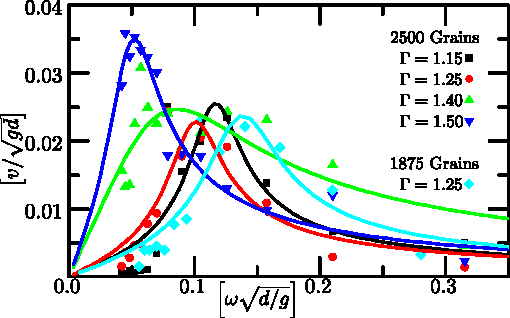
\includegraphics[width=0.65\textwidth]{04-figuras/BNE_ResonancePBC.pdf}
    \caption[BNE with periodic boundary: resonance.]{Intruder ascent rate $v$ curves for various normalized external accelerations $ \Gamma $, for the pbc case. $\Gamma = 1.15$ and $2500$ grains is in $\textcolor{black}{\blacksquare}$, $\Gamma = 1.25$ and $2500$ grains is in $\textcolor{red}{\bullet}$, $\Gamma = 1.40$ and $2500$ grains is in $\textcolor{green}{\blacktriangle}$, $\Gamma = 1.50$ and $2500$ grains is in $\textcolor{blue}{\blacktriangledown}$, $\Gamma = 1.25$ and $1875$ grains is in $\textcolor{cyan}{\Diamondblack}$, all with $37.5d$ wide. Figure also present in \cite{Large-deviation_quantification_of_boundary_conditions_on_the_Brazil_nut_effect}.}
    \label{fig:BNE_resonance}
\end{figure}

    Figure \ref{fig:BNE_resonance} shows us that the ascent rate changes with the applied frequency, and as sudden the intruder ascent to the top, we propose that the behavior of the BNE in pbc could be modelled as a resonant system, since that dependency on $\omega$ is expected for a typical resonant system. Then, in analogy, the system behaves like a forced damped harmonic oscillator, with the response in the element that dissipates energy. The equation of a linear damped harmonic oscillator is:
%
\begin{equation}
    \frac{d^2 y}{d t^2} + 2 \zeta \omega_0 \frac{d y} {d t} + \omega_0^2 y = \Gamma \sin(\omega t) ~,  
\end{equation}
%
where $\omega_0$ is the natural frequency of the system, $\zeta$ is the damping ratio, a parameter of the fitting function. The solution to this equation can be written is several forms depending on the element over which is measured the response. Considering the resonant system in analogy to a mass-spring-damper system, if we measure the transfer function over the damper element, which represents the ascent rate of the intruder, the solution for the gain reads:
%
\begin{equation}
    G(\omega) = \frac{2 \zeta \omega_0 \omega }{ \sqrt{(2 \zeta \omega_0 \omega)^2 + (\omega_0^2 - \omega^2)^2 }}~,
    \label{equ:TF}
\end{equation}
%
that we have used to fit the data in Figure \ref{fig:BNE_resonance}. Note the bell shape of the fitting curves, analogous to the sharpness curve for the amplitude magnitude typical in traditional resonance analysis. We use the fact that pbc systems does not have convection current, and the main effect to ascent the intruder is the ratchet effect.

    The data could be collapsed around the fitted parameter $\omega_0$ and results in the curve shown in Figure \ref{fig:BNE_collapse}. The fitting parameters are shown in Figure \ref{fig:BNE_fit_parameters}. Even harder grains obeys this trend. The dynamics of the resonance does not follow exactly the linear approximation, as we can observe in log-log scale, but near the peak the adjust is good.

\begin{figure}
    \centering
    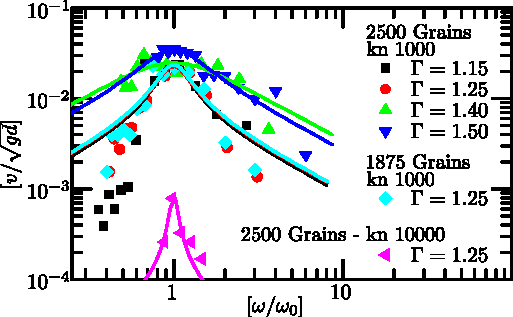
\includegraphics[width=0.65\textwidth]{04-figuras/BNE_Collapse.pdf}
    \caption[BNE with periodic boundary: resonance collapse.]{Collapse of the measured values. The data points are collapsed for all simulations with pbc. The fit can cover the ascent rate for different parameters, like stiffness $k_n$, normalized acceleration $\Gamma$, and the column above the intruder $h$. Figure also present in \cite{Large-deviation_quantification_of_boundary_conditions_on_the_Brazil_nut_effect}.}
    \label{fig:BNE_collapse}
\end{figure}

\begin{figure}
    \centering
    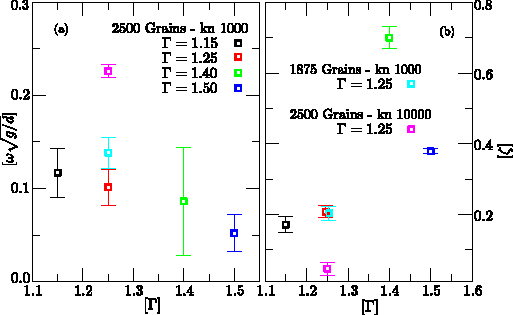
\includegraphics[width=0.65\textwidth]{04-figuras/BNE_Fit.pdf}
    \caption[BNE with periodic boundary: resonance fitting parameters.]{Fit of the parameters of using Equation (\ref{equ:TF}). In (a), the fitted natural frequency $\omega_0$ shows little dependence with $\Gamma$. In (b), the dissipation parameter shows agreement within the error bars to a constant value. Figure also present in \cite{Large-deviation_quantification_of_boundary_conditions_on_the_Brazil_nut_effect}.}
    \label{fig:BNE_collapse}
\end{figure}

    The damping effect $\zeta$ in the fit does not relate to the damping factor $\gamma$ (or restitution coefficient $\epsilon$) of the grains contact, once the $\gamma$ is critical and would lead to dissipation of energy enough to resonance does not happen in the contact interaction. A further investigation into this system linking force balance or energy balance to the proposed resonance is needed. We propose a scale in the frequency $\omega \propto \sqrt{k_n^3}/h$ while the ascent rate $v \propto \frac{d}{h g}\left(\sqrt{\frac{k_n/m}{\Gamma}}\right)^3$, where $k_n$ is the stiffness of the grains, $h$ is the difference between the top layer of grains and the intruder position, $d$ is the grain diameter, $g$ is the gravity, $m$ is the mass of the grains, and $\Gamma$ is the dimensionless shaken acceleration compared to the gravity.

\begin{figure}
    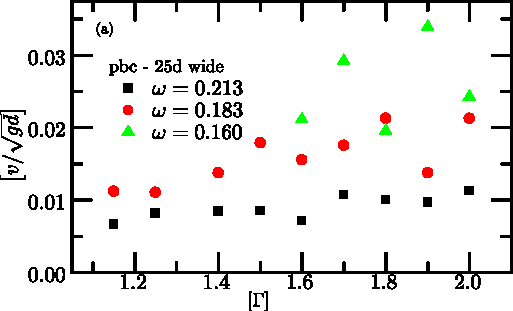
\includegraphics[width=0.65\linewidth]{04-figuras/BNE_PBC25.pdf}
    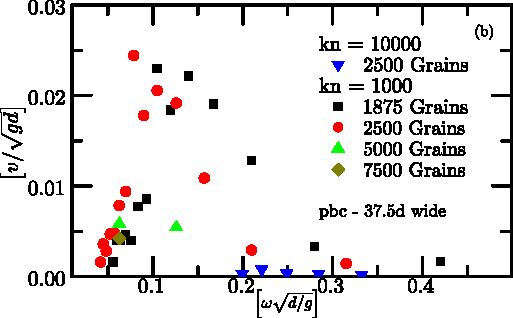
\includegraphics[width=0.65\linewidth]{04-figuras/BNE_PBC37.pdf}
    \caption[BNE with periodic boundary: 25$d$ and 37.5$d$.]{In (a), 25d wide in pbc. Increase $\Gamma$ leads to increase ascent rate. In (b) 37.5 wide in pbc. Figure also present in \cite{Large-deviation_quantification_of_boundary_conditions_on_the_Brazil_nut_effect}.}
    \label{fig:BNE_pbc}
\end{figure}

    And at least comparison in Figure \ref{fig:BNE_pbc}, another exploration on the parameters: width of 25$d$ and different number of grains in width of 37.5$d$, all in pbc.

    To reinforce the idea of the resonance, we analyse the fluctuation properties of the ratchet effect using Large Deviation Function (LDF) \cite{Symmetry_properties_of_the_large-deviation_function_of_the_velocity_of_a_self-propelled_polar_particle, Large_Deviations_in_Physics}. We quantify the fluctuations of the ascent rate distribution of the intruder measuring the normalized  $W_{\tau}$ as:
%
\begin{equation}
    W_{\tau}(t) = \frac{1}{\tau} \int_t^{t+\tau} \frac{v(t')}{\left<v\right>} dt'~, 
\end{equation}
%
where $v(t)$ is the intruder vertical velocity at time $t$ and $\left< \cdot \right>$ denotes the average over $[0,t+\tau]$. Next, we have calculated $P(W_{\tau})$, the density probability function of $W_\tau$, and obtained the RF at the limit
%
\begin{equation}
    RF(W_\tau) = -\lim_{\tau \rightarrow \infty} \frac{1}{\tau} \ln P(W_\tau)~.
\end{equation}

    We could collapse the curves for long range integration times, when we can see the BNE regime acting in the system. The short time integration did not collapse, once the predominant dynamic is the external oscillation. Figure \ref{fig:LDFgamma} shows the LDF in fw and pbc. When fw are in play, the asymmetry between falling and rising is pronounced, shown with the metric $P(W_{\tau})$ in Figure \ref{fig:LDFgamma}(b). On the other hand, when pbc is consider, the asymmetry of upward and downward is only observed on a high value of $\tau$, Figure \ref{fig:LDFgamma}(d). The $RF$ reaches its value in small $W_{\tau}$ for fw, Figure \ref{fig:LDFgamma}(a), while only long values of $W_{\tau}$ exhibit larger jumps in pbc.

\begin{figure}
    \centering
    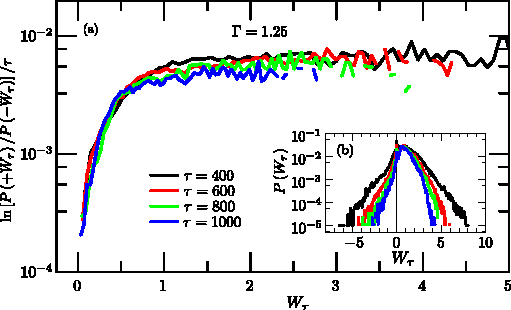
\includegraphics[width = 0.49\linewidth]{04-figuras/BNE_LDF_FW.pdf}
    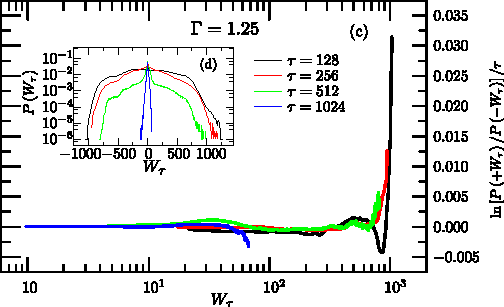
\includegraphics[width = 0.49\linewidth]{04-figuras/BNE_LDF_PBC.pdf}
    \caption[BNE with periodic boundary: large deviation.]{Inset: $P(W_\tau)$ for $\Gamma = 1.25$ and several values of $\tau$ as shown in the legends, for both systems: with frictional walls at left and pbc at right. Main panels: collapse of the RF function calculated for $\Gamma = 1.25$, and several values of $ \tau$.  Data collapse was performed by dividing the ratio between upward and downward probabilities by the integration time $\tau$. For the range of integration times considered, a remarkable collapse is observed. The frictional walls case is shown at left and pbc at right panel. Observe that distributions for pbc are much more symmetric than those for fw, which lean strongly to the positive side. Figure also present in \cite{Large-deviation_quantification_of_boundary_conditions_on_the_Brazil_nut_effect}.}
    \label{fig:LDFgamma}
\end{figure}

%    No próximo capítulo, descreveremos os modos de transporte de grãos quando arrastados por um fluido.

    Next Chapter we describe the techniques to simulate the fluid.
            % Resultados
\chapter{Methodology - CFD}
\label{chap:CFD}

    In this Chapter we describe the model we chose to simulate the fluid, the hypotheses and approximations, the discretization of equations, some methods to solve them, the algorithm and the results of the fluid. The we chose to simulate a Finite Difference Method (FDM) with an Eulerian\footnote{
    Eulerian method: a fixed mesh in space with the representative flow evolves in time. The reference point is in the position space.

    Lagrangian method: a fixed mesh that moves with the frame and represents the flow in time. The reference point is in the velocity space.

    Lattice Boltzmann method: a fixed lattice is set to represent the collision and streaming in time.
} method.

\section{The fluid model}
    The general equation that governs the system is the Navier-Stokes equations, which is the application of Newton's second law to specific mass in continuous media and the application of the conservation laws of mass and momentum \cite{Physical_Hydrodynamics, Fluid_Mechanics}. For the equation of mass conservation, we have the Equation \ref{equ:conservacao_massa}: 
\begin{equation}
    \frac{\partial \rho^{f}}{\partial t} +\vec{\nabla}.(\rho \vec{u}^{f}) = 0,
    \label{equ:conservacao_massa}
\end{equation}
where $\rho^{f}$ is the fluid density, and $\vec{u}^{f}$ is the fluid velocity.

    The Equation \ref{equ:conservacao_momento} describes the momentum conservation as:
\begin{equation}
    \frac{\partial}{\partial t}\left(\rho^{f}\vec{u}^{f}\right) +\vec{\nabla}.\left(\rho^{f}\vec{u}^{f}\otimes\vec{u}^{f}\right) = \overline{\overline{\sigma}} +p_{ext},
    \label{equ:conservacao_momento}
\end{equation}
where $\rho^{f}$ is the fluid density, $\vec{u}^{f}$ is the fluid velocity, $\overline{\overline{\sigma}}$ is the fluid stress tensor (pressure $p$ and viscosity $\tau$ terms) and $p_{ext}$ is the external pressure, or the body pressure like gravity or drag forces induced by presence of grains.

    In formulating the momentum conservation, there is internally the mass conservation, and if we write the terms of the equation making the inner products and the derivatives, we have the Equation: 
\begin{equation}
    \rho^{f} \frac{\partial \vec{u}^{f}}{\partial t} +\rho^{f}\left(\vec{u}^{f}.\vec{\nabla}\right)\vec{u}^{f} = \vec{\nabla}.\overline{\overline{\sigma}} +p_{ext},
    \label{equ:Navier-Stokes}
\end{equation}
where $\rho^{f}$ is the fluid density, $\vec{u}^{f}$ is the fluid velocity, $\overline{\overline{\sigma}}$ is the fluid stress tensor (pressure $p$ and viscosity $\tau$ terms) and $p_{ext}$ is the body pressure. The fluid stress tensor $\overline{\overline{\sigma}}$ is written in 2D like:
\begin{equation}
    \overline{\overline{\sigma}} = \left(
    \begin{matrix}
        \sigma_{xx} & \tau_{xz} \\
        \tau_{zx} & \sigma_{zz}
    \end{matrix}
    \right),
    \label{equ:tensor_tensao}
\end{equation}
where $\overline{\overline{\sigma}}$ is the fluid stress tensor, $\sigma_{xx}$ and $\sigma_{zz}$ are the pressure components in the $x$ and $z$ directions, respectively, and the fluid pressure is $p=-\frac{1}{2}(\sigma_{xx}+\sigma_{zz})$, while the shear components are $\tau_{xz}$ and $\tau_{zx}$.

    The equations above describe most of the fluids, but other enclosures must be done to determine which technique is going to be applied, since the Navier-Stokes equations are not analytically solvable yet and in some cases we have more variables than equations. With this hint in mind, we decided to model the fluid as a incompressible Newtonian fluid. Additionally, we consider that there is no circulation of the fluid in the direction of the gravity (the fluid flows only in $x$ direction), have periodic boundary condition (pbc) in $x$ direction (what happens in the left boundary is exactly same condition to the right boundary) and is constant in the $x$ direction, setting a quasi-1D fluid flow, that changes in the $z$ direction, but only flows in $x$. The pbc implies in some simplifications on Equations \ref{equ:conservacao_massa}, \ref{equ:conservacao_momento} e \ref{equ:Navier-Stokes}. Automatically, to the Equation \ref{equ:conservacao_massa}, the incompressible Newtonian fluid approach leads to any variation in the fluid density $\rho^f$ to be null, so $\frac{\partial \rho^f}{\partial t} $ = 0, and if this part is null, then $\vec{\nabla}.(\rho \vec{u}^{f})$ = 0 is so, and as $\frac{\partial u_z^f}{\partial z}$ = 0, $\frac{\partial u_x^f}{\partial x}$ is also null, and it contributes to the assumption that the fluid should be the same in $x$ direction. Also the shear stress $\tau_{xz}$ = $\tau_{zx}$ is symmetric. The component of the pressure $\sigma_{xx}$ = 0, due to the pbc, in Equation \ref{equ:Navier-Stokes}. With all this simplification, we have the total shear stress written as:
\begin{equation}
    \vec{\nabla}.\overline{\overline{\sigma}} = \frac{\partial \tau}{\partial z} \hat{x} - \frac{\partial p}{\partial z} \hat{z}
    \label{equ:divergente_tensor_tensao}
\end{equation}
where $\overline{\overline{\sigma}}$ is the stress tensor of the fluid, $\tau$ is the shear flow component, $p$ is the pressure of the fluid (which has only component in $z$ direction), $\hat{x}$ is the flow direction and $\hat{z}$ is the gravity direction.

    An important measure is the fluid strain rate, given by: 
\begin{equation}
    \dot{\gamma}_{xz} = \frac{1}{2} \left(\frac{\partial u_{x}}{\partial z} +\frac{\partial u_{z}}{\partial x} \right),
    \label{equ:taxa_deformacao}
\end{equation}
where $\dot{\gamma_{xz}}$ and $\dot{\gamma_{zx}}$ are the components of the strain rate tensor, $u_{x}$ is the fluid velocity in the flow direction and $u_{z}$ is the fluid velocity in the direction of gravity.

    In this approach, the shear flow controls some characteristics of the fluid, such as the transition from laminar to turbulent approach. The following equation relates the shear and the strain rate:
\begin{equation}
    \tau = \rho^{f}(\nu+\nu_{t})\dot{\gamma},
    \label{equ:cisalhamento}
\end{equation}
where $\tau$ is the shear flow, $\rho^{f}$ is the fluid density, $\nu$ is the intrinsic viscosity of the fluid, $\nu_t$ is the contribution of the turbulent model, in therms of viscosity, and $\gamma$ is the strain rate. To model a Newtonian fluid, the turbulent part must be null.

    Appling the assumed hypothesis about the fluid in the Navier-Stokes equations (Equation \ref{equ:Navier-Stokes}), the following system according to the flow direction ($x$) and gravity ($z$):
\begin{subequations}
    \begin{empheq}[left={}\empheqlbrace]{align}
        \rho^{f} \frac{\partial u_{x}^{f}}{\partial t} &= \frac{\partial \tau}{\partial z} & : \hat{x},
        \label{equ:fluido_x} \\
         0 &= -\frac{\partial \sigma_{zz}}{\partial z} + \rho^{f}g & : \hat{z},
         \label{equ:fluido_y}
    \end{empheq}
    \label{equ:fluido}
\end{subequations}
where $\rho^f$ is the fluid density, $u_x^f$ is the velocity in the flow direction, $\tau$ is the shear stress, $\sigma_{zz}$ is the stress component in the direction of the gravity and $g$ is the value of the gravity acceleration.

    As expected, the change of pressure depends on gravity and fluid density. Integrating Equation \ref{equ:fluido_y}, the pressure is:
\begin{equation}
    \sigma_{zz} = \rho^f g z.
\end{equation}

    For the fluid strain rate, applying fluid considerations results in:
\begin{equation}
    \dot{\gamma_{xy}} = \frac{\partial u_{x}}{\partial z},
    \label{equ:taxa_deformacao_final}
\end{equation}
where $\dot{\gamma_{xy}}$ is the strain rate tensor component, $u_x$ is the fluid velocity in the flow direction and $z$ is the gravity direction.

    Now, lets analyze the regimes of the fluid: viscous steady-state and viscous transient.

\subsection{Viscous steady-state regime}
\label{sec:viscous_steady}
    For the viscous regime, all turbulence vanishes, than only viscosity plays a role in the shear. To find a steady-state than, the variation of the velocity in time must be zero, or:
    \begin{equation}
        \frac{\partial u}{\partial t} = 0,
        \label{equ:dudt0}
    \end{equation}
meaning that:
    \begin{equation}
        \frac{\partial \tau}{\partial z} = 0,
        \label{equ:dtaudz0}
    \end{equation}
and if the variation on $\tau$ is independent of the time and space, in this special case of no turbulence, we can write Equation \ref{equ:viscous_steady0} in function of the variation of the velocity over the space as:
    \begin{equation}
        \frac{\partial u}{\partial z} = \frac{\tau}{\rho \nu},
        \label{equ:viscous_steady0}
    \end{equation}
with $\tau = \rho {u_{*}}^{2}$ imposed on top ($u_{*}$ been the characteristic velocity of the imposed shear), and it is constant everywhere. Integrating equation and applying the bottom boundary condition, $u=0$, we get:
    \begin{equation}
        u^+ = z^+,
        \label{equ:viscous_steady1}
    \end{equation}
with $u^+ = u/u_{*}$ and $z^+ = z u_{*}/\nu$.

\begin{figure}[H]
    \centering
    \parbox{0.495\textwidth}{
        \centering
        \includegraphics[width= 0.45\textwidth]{04-figuras/viscous_steady_velocity.tikz}
        \subcaption{Normalized velocity of viscous steady-state profile.}
        \label{fig:viscous_steady_velocity}
    }
    \parbox{0.495\textwidth}{
        \centering
        \includegraphics[width= 0.45\textwidth]{04-figuras/viscous_steady_shear.tikz}
        \subcaption{Normalized shear of viscous steady-state profile.}
        \label{fig:viscous_steady_shear}
    }
    \caption[Steady-state analytical solution for viscous fluid profiles.]{Velocity and shear steady-state profiles for the viscous fluid. With viscosity, the response of the velocity profile tends to be a line, and the steady-state makes the shear profile a constant.}
    \label{fig:viscous_steady}
\end{figure}

    As we are not limited by an upper boundary, the fluid has an infinity characteristic length in the steady-state regime.

    So then, we now know the exact solution in the steady-state for the viscous fluid. The fluid velocity profile and the fluid shear profile must follow as in figure \ref{fig:viscous_steady}. As said before, the shear profile is constant everywhere, and the velocity profile is a line.

\subsection{Viscous transient regime}
    Having the stationary solution in hands, we can think if there is a possibility to describe the transient regime of the equation \ref{equ:fluido_x}. This is a linear partial differential equation: the diffusion equation. Equation \ref{equ:viscous_transient_velocity_full_solution} is the general solution\footnote{For more details, Attachments \ref{chap:Calculations} have the whole calculation to get in the solution we got. It is also described in \cite{Boyce}, Chapter 10.} with the boundary conditions and generic initial velocity profile $u_0(z)$.
\begin{equation}
    \begin{split}
        u^+ = z^+ +\frac{2}{h}\sum_{n=1}^\infty\Bigg\{
        &{\int_0^h\left[\frac{u_0\left(\zeta\right)}{u_*}-\frac{u_*}{\nu}\zeta\right]\sin\left(\pi\frac{2n-1}{2h}\zeta\right) \mathrm{d}\zeta}\\
        &{\sin\left(\pi\frac{2n-1}{2h}z\right)}
        {e^{-{\left(\pi\frac{2n-1}{2h}\right)}^2\nu t}}
        \Bigg\},
    \end{split}
    \label{equ:viscous_transient_velocity_full_solution}
\end{equation}
where $z^+$ is the normalized steady-state solution, $u_0(\zeta)/u_*$ is the normalized initial velocity profile that covers all the domain between $0$ and $h$, $h$ is the height where we impose the shear to propagate through all of the system, and the integral is the transformation of the function transient into the Fourier coefficients.

    The first difference here appears in delimiting an height $h$ at the top. With it, we know that time to change from the initial condition to the stationary regime is dependent of $h^2$, so, higher we impose shear, greater is the time to converge to the final solution. If $h\to\infty$, also the time to converge goes to infinity. It also plays a role in the modes of the Fourier solution.

    Looking at the presented solution in equation \ref{equ:viscous_transient_velocity_full_solution}, we can see that it decays with an exponential in time, obeying the differential partial equation \ref{equ:fluido_x} according through time, and it is oscillates with an infinite sum of sin in function of space, which is the solution for differential equation of second order in the same equation \ref{equ:fluido_x}.

    For the initial condition, we choose the one stationary regime with imposed shear as $\tau = \rho {\left(u_*-\Delta u_*\right)}^2$, and then $u_0(z)=(u_*-\Delta u_*)^2 z/\nu$. In terms of Fourier coefficients, we have:
    \begin{equation}
        -\frac{8}{\pi^2}h^+ \epsilon\left(2-\epsilon\right)\frac{\left(-1\right)^{n-1}}{\left(2n-1\right)^2},
    \end{equation}
that is linear in $z$, because $u_0(z) = z(u_*-\Delta u_*)^2/\nu$ is linear in $z$. Then, with this, the solution become as following:
\begin{equation}
    \begin{split}
        u^+ = z^+ -\frac{8}{\pi^2}h^+\epsilon\left(2-\epsilon\right)\\
        \sum_{n=1}^\infty\left[
        {\frac{\left(-1\right)^{n-1}}{\left(2n-1\right)^2}}
        {\sin\left(\pi\frac{2n-1}{2h}z\right)}
        {e^{-{\left(\pi\frac{2n-1}{2h}\right)}^2\nu t}}
        \right]
    \end{split}
    \label{equ:viscous_transient_velocity}
\end{equation}

    If we get the the Fourier mode with higher amplitude and slowest response in equation \ref{equ:viscous_transient_velocity}, than we can write the velocity as the function:
    \begin{equation}
        u^+ = \left[z^+ -\frac{8}{\pi^2}h^+\epsilon\left(2-\epsilon\right)\sin\left(\frac{\pi}{2h}z\right)e^{-{\left(\frac{\pi}{2h}\right)}^2\nu t}\right]
        \label{equ:viscous_transient_velocity1}
    \end{equation}

    Also, the shear have a temporal evolution, since it is function of the velocity. If we take the derivative of the velocity in function of the space, we can extract the function of shear in time and in space. The 1$^{st}$ Fourier mode of the shear evolves as:
    \begin{equation}
        \tau^+ = \left[1 -\frac{4}{\pi}\epsilon\left(2-\epsilon\right)\cos\left(\frac{\pi}{2h}z\right)e^{-{\left(\frac{\pi}{2h}\right)}^2\nu t}\right]
        \label{equ:viscous_transient_shear1}
    \end{equation}

    So, if $\epsilon \ll 1$, then the steady-states are close each other, and the linearization around $\Delta u_*$ simplifies the transition between two steady states close each other. The reason to get the first Fourier mode is to determine the temporal dominant behavior over the equation.

    Than, with the linear approximation described in Equations \ref{equ:viscous_transient_velocity1} and \ref{equ:viscous_transient_shear1}, we can see the temporal evolution of the profiles in Figures \ref{fig:viscous_transient0} and \ref{fig:viscous_transient}.

\begin{figure}[H]
    \centering
    \includegraphics{04-figuras/viscous_transient.tikz}
    \caption[Temporal solution for viscous fluid profiles.]{Temporal evolution of the mean velocity and shear at bottom through time with height $h=25$ and $\Delta u_*=0.1 u_*$. The curves matches as expected, an exponential decay, from one given point to the asymptotic. Higher modes than the 1$^{st}$ Fourier mode contributes heavily in the beginning but decay fast, and for the main behavior, the 1$^{st}$ Fourier mode gives a good approximation of the temporal evolution. Here we introduce a curve created by the discretization of the equations, that is going to be discuss in section \ref{sec:discrete}.}
    \label{fig:viscous_transient}
\end{figure}

    Looking at the response on Figure \ref{fig:viscous_transient}, one can see that it evolves like an exponential, but to be sure, we plot the variables in semi-log scale. Figure \ref{fig:viscous_transient0} shows the response without the stationary value, focusing the nature of the transition regime.

\begin{figure}[H]
    \centering
    \parbox{1\textwidth}{
        \centering
        \includegraphics[width=0.495\textwidth]{04-figuras/viscous_transient_velocity0.tikz}
        \subcaption{Normalized mean velocity. In green we have Euler discretization method, in blue we have all Fourier modes and in red we have 1$^{st}$ Fourier mode of viscous transient-state subtracted the stationary regime. For the Fourier modes we have $h=10$ dotted, $h=25$ lined and $h=100$ dashed with $\Delta u_*/u_*$ varying from $10^{-1}$ to $10^{-3}$.}
        \label{fig:viscous_transient_velocity0}
    }
    \parbox{1\textwidth}{
        \centering
        \includegraphics[width=0.495\textwidth]{04-figuras/viscous_transient_shear0.tikz}
        \subcaption{Normalized shear of the bottom layer. In green we have Euler discretization method, in blue we have all Fourier modes and in red we have 1$^{st}$ Fourier mode of viscous transient-state subtracted the stationary regime. For the Fourier modes we have $h=10$ dotted, $h=25$ lined and $h=100$ dashed with $\Delta u_*/u_*$ varying from $10^{-1}$ to $10^{-3}$.}
        \label{fig:viscous_transient_shear0}
    }
    \caption[Normalized profiles for viscous fluid.]{Normalized velocity and shear stress evolution of viscous transient-state profile through time. All curves collapses at the same one, showing that there is only one behavior that domains the response: the exponential decay. Indeed, as we have expected from the equation in time to go from one stationary regime to another stationary regime from an exponential decay.}
    \label{fig:viscous_transient0}
\end{figure}

    It is also important to look at the approximation of the Fourier's 1$^\textrm{st}$ mode in velocity $\mathcal{U}_1$ (Equation \ref{equ:mode1}) in comparison with the original function, that in this case is a line (Equation \ref{equ:viscous_steady1}) for velocity, and is a constant for shear. Equation \ref{equ:mode1} contains the first mode linearized in $\Delta u_*$ and figure \ref{fig:mode1} has the visual comparison between approximation of the 1$^{st}$ mode and the full solution.

\begin{equation}
    \mathcal{U}_1 = -\frac{u_*^2}{\nu}\frac{\Delta u_*}{u_*}h\frac{16}{\pi^2}\sin\left(\frac{\pi}{2h}z\right)
    \label{equ:mode1}
\end{equation}

\begin{figure}[H]
    \centering
    \includegraphics[width=0.65\textwidth]{04-figuras/mode1.tikz}
    \caption[Comparison between 1$^{st}$ Fourier mode and exact solution for viscous fluid velocity.]{Amplitude of the first Fourier mode in comparison with exact solution. In red, the initial amplitude of the first Fourier mode, in blue the initial amplitude of the all modes.}
    \label{fig:mode1}
\end{figure}

    With the description of the viscous transient regime described and approximated to the first Fourier mode and linearised around the ratio $\Delta u_*/u_*$, now it is time to introduce the turbulence term and see how it evolves in time.

    For the stationary turbulent model, using Prandtl turbulent model, the Reference \cite{Numerical_simulation_of_turbulent_sediment_transport} and see the Appendix \ref{chap:Turbulence}.

\section{Force model - Fluid forces}
\label{subchap:Modelo_Forcas}
    The forces modelled in this thesis include the contact forces between agents (Chapter \ref{chap:DEM}, which belong to the rheological model of grains), the interaction forces between grain and fluid, and the gravitational force. 

\label{subsubchap:Fluido}
    The force that the fluid exerts on the grains can be understood as a contribution from different models and cases. A more detailed formulation of each portion of forces that the fluid exerts on each body is described by the equation:
\begin{equation}
    \vec{F}_{i}^{Fluid} = \vec{F}_{i}^{Arch} +\vec{F}_{i}^{Drag} +\vec{F}_{i}^{Magnus} +\vec{F}_{i}^{Lift} +\vec{F}_{i}^{AddedMass} +\vec{F}_{i}^{Basset},
    \label{equ:forcas_fluido}
\end{equation}
where $\vec{F}_{i}^{Fluid}$ is the total forces contribution that the fluid exerts on the grain $i$, $\vec{F}_{i}^{Arch}$ is the Archimedes' force that acts on the grain $i$, $\vec{F}_{i}^{Drag}$ is the drag force on the grain $i$, $\vec{F}_{i}^{Magnus}$ is the Magnus' force on the grain $i$, $\vec{F}_{i}^{Lift}$ is the lift force on the grain $i$, $\vec{F}_{i}^{AddedMass}$ is the added mass force on the grain $i$ and $\vec{F}_{i}^{Basset}$ is the Basset's force on grain $i$. As a simplification of the model, we will use only Archimedes' and fluid drag forces \cite{Fluid_Mechanics, Numerical_simulation_of_turbulent_sediment_transport, Maurin-Tese}.

    Archimedes' force can be written as in the equation \ref{equ:arquimedes}, while the drag force can be written as in the equation \ref{equ:arraste}: 
\begin{equation}
    \vec{F}_{i}^{Arch} = \frac{\pi}{6} d_{i}^{3} \vec{\nabla}.\overline{\overline{\sigma}},
    \label{equ:arquimedes}
\end{equation}
where  $\vec{F}_{i}^{Arch}$ is the Archimedes' force on grain $i$, $d_i$ is the diameter of the grain $i$ and $\vec{\nabla}.\overline{\overline{\sigma}}$ is the divergent of the fluid stress tensor $\overline{\overline{\sigma}}$, and:
\begin{equation}
    \vec{F}_{i}^{Drag} = \frac{\pi}{8}\rho_{f}d_{i}^{2}C_{d}(\mathcal{G}_{u})\left|\vec{u}_{f}-\vec{v}_{i}\right|(\vec{u}_{f}-\vec{v}_{i}),
    \label{equ:arraste}
\end{equation}
where $\vec{F}_{i}^{Drag}$ is the drag force on grain $i$, $\rho_f$ is the fluid density, $d_i$ is the diameter of the grain $i$, $C_{d}(\mathcal{G}_{u})$ is the drag coefficient based on the body Galileo number, described by Equation \ref{equ:reynolds_arraste}, $\vec{u}_{f}$ is the fluid velocity, $\vec{v}_{i}$ is the grain velocity \cite{Numerical_simulation_of_turbulent_sediment_transport}.

\begin{equation}
    C_{u}(\mathcal{G}_{u}) = \left( \sqrt{C_{d}^{\infty}} +\sqrt{\frac{\mathcal{G}_{u}^{c}}{\mathcal{G}_{u}}} \right)^{2}
    \label{equ:reynolds_arraste}
\end{equation}
where $C_{u}(\mathcal{G}_{u})$ is the drag coefficient based on the body Galileo number, $C_{d}^{\infty} \simeq$ 0.5 is the drag coefficient in the turbulent limit ($\mathcal{G}_{u} \to \infty$), $\mathcal{G}_{u}^{c} \simeq$ 24 is the body transition Galileo number, in which the drag coefficient becomes almost constant, and Equation \ref{equ:reynolds_fluido_grao} relates the body Galileo number to the parameters of the system:
\begin{equation}
    \mathcal{G}_{u} = \frac{d_{i}}{\nu} \left| \vec{u}_{f} -\vec{v}_{i} \right|
    \label{equ:reynolds_fluido_grao}
\end{equation}
where $d_i$ is the diameter of the grain $i$, $\nu_{tot}$ is the dynamic viscosity of the system ($\nu+\nu_t$), $\vec{u}_{f}$ is the fluid velocity and $\vec{v}_i$ is the velocity of the grain $i$.

    With these equations, grain and fluid exchange motion. By third Newton's law, grains exert body forces on the fluid, and fluid reacts with fluid forces on the grains. By the computation of the fluid forces, we couple the exchange of momentum between grain and fluid, applying the fluid force on the grain divided by the area of the grain into the fluid.

\subsection{Temporal discretization}
\label{sec:discrete}
    To numerically solve the fluid equations, a mesh is constructed in $z$ direction, and average it in the $x$ direction each time step. This average make the system to be smoother, but at same time it gives the probability to have particles' properties in function of $z$. This smoothness makes the solution more stable to interact the fluid with the grains and update both of them. The first way to think in the discrete equations is the explicit\footnote{The explicit way of solving a FDM solves the system for the next time step with the original differential equation operations. All discretization is done on the functions of the current time step resulting in the later time step. The disadvantage of this technique is the instability factor of the solution that can occur. The advantage is that the system can always be written by these equations.} form. Then Equations \ref{equ:fluido_x} and \ref{equ:viscous_steady0} becomes:    
\begin{subequations}
    \begin{empheq}[left={}\empheqlbrace]{align}
        {U_{x}}_{\;k}^{n+1} &= {U_{x}}_{\;k}^{\;n} + \frac{\Delta t}{\rho^{f}\Delta z} \left[\tau_{\;k}^{\;n} -\tau_{k-1}^{\;n}\right] - \frac{\Delta t}{\rho^{f}}\frac{\phi_{\;k}^{\;n}}{1-\phi_{\;k}^{\;n}}{f_x}_{\;k}^{\;n},
        \label{equ:fluido_discreto_velocidade} \\
        \tau_{\;k}^{\;n} &= \rho^{f} \left[\nu\right]\left(\frac{{U_{x}}_{k-1}^{n}-{U_{x}}_{\;k}^{\;n}}{\Delta z}\right),
        \label{equ:fluido_discreto_cisalhamento}
    \end{empheq}
    \label{equ:fluido_discreto_explicito}
\end{subequations}
where $k$ is the fluid spatial discretization index, $n$ is the time step, ${U_x}_{\;k}^{n+1}$ is the fluid flow velocity in height $k \Delta z$ and time $(n+1)\Delta t$, ${U_x}_{\;k}^{n}$ is the fluid flow velocity in height $k \Delta z$ and time $n\Delta t$, $\Delta z$ is the fluid meshing space, $\Delta t$ is the time step interval, $\rho^f$ is the fluid density, $\phi$ is the packing fraction that solid part occupies, $\tau$ is fluid shear, $f_x$ is the force per volume in the $x$ direction that grains exert on the fluid, $\nu$ is the fluid viscosity. The stability condition must be obeyed:
\begin{subequations}
    \begin{empheq}{align}
        \frac{2\Delta t}{\left(\Delta z\right)^{2}} < 1,
        \label{equ:estabilidade_laminar} \\
        \frac{2\Delta t}{\left(\Delta z\right)^{2}} < 1,
        \label{equ:estabilidade_turbulento}
    \end{empheq}
    \label{equ:estabilidade}
\end{subequations}
if there is no grains to exert body force on the fluid, otherwise the stability must be much more rigorous, once numerical errors are amplified due to discretization \cite{Transferencia_de_calor_e_mecanica_dos_fluidos_computacional, Numerical_Methods_for_Scientists_and_Engineers, Numerical_Recipes, Numerical_Solution_of_Partial_Differential_Equations}.

    But as the explicit form of the equation is unstable, we can rewrite it in the implicit\footnote{The implicit way of solving a FDM solves the next time step system based on the differential equation roots of the problem. All discretization is done considering the roots that solve the equation. The disadvantage of this technique is the fact that there is not always an algorithm that finds the roots. The advantage is that the stability factor is more permissive.} form:
\begin{equation}
    {U_{x}}_{\;k}^{\;n} -\frac{\Delta t}{\rho^f}\frac{\phi_{\;k}^{\;n}}{1-\phi_{\;k}^{\;n}}{f_x}_{\;k}^{\;n} = -\frac{\Delta t \nu}{\left(\Delta z\right)^2}{U_{x}}_{\;k-1}^{\;n+1} \left(1+2\frac{\Delta t \nu}{\left(\Delta z\right)^2}\right){U_{x}}_{\;k}^{\;n+1} -\frac{\Delta t \nu}{\left(\Delta z\right)^2}{U_{x}}_{\;k+1}^{\;n+1},
    \label{equ:fluido_discreto_implicito}
\end{equation}
where $k$ is the fluid spatial discretization index, $n$ is the time step, ${U_x}_{\;k}^{n+1}$ is the fluid flow velocity in height $k \Delta z$ and time $(n+1)\Delta t$, ${U_x}_{\;k}^{n}$ is the fluid flow velocity in height $k \Delta z$ and time $n\Delta t$, $\Delta z$ is the fluid meshing space, $\Delta t$ is the time step interval, $\rho^f$ is the fluid density, $\phi$ is the packing fraction that solid part occupies, $\tau$ is fluid shear, $f_x$ is the force per volume in the $x$ direction that grains exert on the fluid, $\nu$ is the fluid viscosity. But as we can inspect, it is not possible to direct extract the result from this equation, since we have a temporal dependency. For our luck\footnote{Unluckily there is no implicit form for turbulent model. To solve the turbulent part by implicit form, one can use a Newton-Raphson algorithm to find the roots and with the root invert the system. I personally chose to do not include this topic in this thesis, once I have not tested the algorithm nor could find the approximated analytical solution to temporal evolution of the Prandl turbulent model.} there is an implicit form and this equation can be written in a linear matrix form:
\begin{equation}
    \left[Tridiag\right].\left[{U_x}_{\;k}^{n+1}\right] = \left[{U_x}_{\;k}^{n} -\lambda \frac{\phi}{1-\phi} {f_x}_{\;k}^{n}\right],
\end{equation}
where $\left[Tridiag\right]$ is a tridiagonal matrix and $\lambda = \frac{\nu \Delta t}{\left(\Delta z\right)^2}$. The tridiagonal matrix have principal diagonal equals to 1+2$\lambda$ and upper and lower diagonals equals to $-\lambda$. Then the inverse of the matrix is applied both sides, and the temporal solution is extracted. To make faster calculations, we use Thomas algorithm (Algorithm \ref{alg:Thomas}) to invert the matrix and extract the product to the vector $U-\lambda \frac{\phi}{1-\phi}f$.

\section{Algorithm}
    Also a series of procedures must be carried out to reach the goal to simulate grain and fluid. As we have discussed in Chapter \ref{chap:DEM}, the simulation of the grain phase should be done, but now taking into the account the fluid force equations into the force calculation routine. The temporal evolution of the fluid phase is adjusted to follow the same time step of the grain phase, and coupling both with the exchange of momentum. The main algorithm that simulates both phases is describe in Algorithm \ref{alg:MD-Fluid}, with the introduction of the fluid phase in blue.

\begin{algorithm}
    \SetKwInOut{Input}{Input}\SetKwInOut{Output}{Output}
    \Input{initial simulation data setup}
    \Output{response and simulation measurements over time}
    \While{not reached the stop condition of the simulation}{
        \textcolor{gray}{
        \If{it is time to List the Neighbors}{
            List the Neighbors\;
        }
        Predictor\;
        Detect Contacts\;
        Force Calculation\;
        Corrector\;
        }
        \textcolor{blue}{Update fluid\;}
    }
%    \caption{Dadas as entradas do problema, como posições iniciais dos corpos, velocidades e acelerações, o algoritmo de Dinâmica Molecular monta uma lista de corpos que são vizinhos delimitados por uma certa região, então prediz a posição e a velocidade dos corpos no próximo instante de tempo, procura os contatos que foram formados com a predição, calcula as forças entre cada corpo em contato e inclui as forças externas, corrige as predições de velocidade e aceleração de cada corpo e calcula a dinâmica do fluido. Assim um passo de Dinâmica Molecular é construído. Retirado de \cite{Dissertacao}.}
    \caption[DEM+CFD algorithm.]{Given the input of the problem, such as initial positions of bodies, velocities and accelerations, the algorithm assembles a list of bodies that are neighbors delimited by a certain region, then predicts the position and velocity of the bodies at the next instant of time, looks for the contacts that were formed with the prediction, calculates the forces between each body in contact and includes the external forces, and corrects the velocity and acceleration predictions for each body and calculate the fluid dynamics. Thus a DEM+CFD step is constructed. Algorithm adapted from \cite{Dissertacao}.}
    \label{alg:MD-Fluid}
\end{algorithm}


\subsection{Force calculation}
    The introduction of the fluid causes additional forces to be calculated in the force calculation routine. The Algorithm \ref{alg:forcas-fluido} introduce the fluid forces on the grains. The insertion of the fluid phase is highlighted in blue.

\begin{algorithm}
    \SetKwInOut{Input}{Input}\SetKwInOut{Output}{Output}
    \Input{positions, velocities and contact list}
    \Output{acting forces and torques in the bodies}
    \ForEach{body}{
        \textcolor{gray}{
        Apply gravity force\;
        \ForEach{body in the contact list}{
            Calculate the normal forces $\vec{N}$\;
            Calculate the rolling forces ${F}^{d}$\;
            \eIf{$|{F}^{d}| < \mu |\vec{N}|$}{
                $\vec{F}^{at} += \vec{F}^{d}\hat{t}$\;
            }{
                $\vec{F}^{at} += \mu \textrm{sign}(\vec{F}^{d}) N\hat{t}$\;
            }
            Calculate torque\;
        }
        }
        \textcolor{blue}{
        Calculate drag force \;
        Calculate Archimedes' force \;
        }
    }
%    \caption[Force calculation.]{Aqui são calculadas as resultantes das forças em cada corpo. A força $\vec{N}$ é a força normal, contribuição da força elástica $\vec{F}^{el}$ e força de amortecimento $\vec{F}^{am}$ (equações \ref{equ:forca_elastica} e \ref{equ:forca_amortecimento}), $F^{d}$ é a força de rolamento de um corpo sobre o outro, que deve ser comparado com a força de atrito estático máxima $\mu N$. Retirado e adaptado de \cite{Dissertacao}.}
    \caption[Force calculation with fluid force]{In this routine, the resultant forces are calculated for each body. The force $\vec{N}$ is the normal force, contribution of the elastic force $\vec{F}^{el}$ and the damping force $\vec{F}^{am}$ (Equations \ref{equ:forca_elastica}, \ref{equ:forca_amortecimento}), $F^{d}$ is the rolling force of one body on the other, which must be compared with the maximum static friction force $\mu N$. Archimedes' and drag forces are calculated every time step on each grain, according to the Equations \ref{equ:arquimedes} and \ref{equ:arraste}. Algorithm adapted from \cite{Dissertacao}.}
    \label{alg:forcas-fluido}
\end{algorithm}


\subsection{The fluid}
    The fluid calculation routine consists of updating the fluid mesh\footnote{The fluid mesh consists of the geometric division of space to perform simulation, and is based on discrete points in space associated with a continuous function. This process is the Finite Discrete Method (FDM) \cite{Numerical_Heat_Transfer_and_Fluid_Flow}.} as a function of the system of Equations \ref{equ:fluido_discreto_explicito} and \ref{equ:fluido_discreto_implicito}. The mesh of this fluid is one-dimensional, since we consider the variation of velocities only in the $z$ direction. Thus, we consider a linear mesh of spacing $\Delta z$, where $\Delta z$ is a fraction of the average grain of the system. For good sampling, we use $\Delta z \simeq$ 0.1$d$, where $d$ is the average grain diameter. To calculate the pressure that the fluid exerts on the grain, we use the fraction of the body that belongs to the layer in which it is inserted. The sum of all body fractions in the layer results in the packing fraction.

\begin{algorithm}
    \SetKwInOut{Input}{Entrada}\SetKwInOut{Output}{Saída}
    \Input{perfil de velocidades e cisalhamento do fluido, forças de arrasto e arquimedes nos grãos, passos de tempo $\Delta t$ e de espaço $\Delta y$}
    \Output{estado do fluido para o próximo passo de tempo}
    \ForEach{corpo}{
        Calcula as pressões dos corpos no fluido\;
    }
    \ForAll{fluido}{
        Calcula o cisalhamento do fluido\;
        Atualiza a velocidade do fluido\;
    }
    \caption{Rotina que atualiza os estados do fluido para o próximo passo de tempo.}
    \label{alg:fluido}
\end{algorithm}


    The explicit way to calculate the fluid is strait forward, just plug in the Equations \ref{equ:fluido_discreto_explicito}, first the shear, later the velocity, since the velocity is dependent on the shear. The implicit way to calculate the fluid needs the attention to the matrix inversion of the system, and it solves the velocity without depending on the shear, so the shear should be extracted after the velocity results. To inverse the matrix, one can do naïvely, with a computational complexity of $\mathcal{O}(n^3)$ or use Thomas' algorithm (Algorithm \ref{alg:Thomas}), with a computational complexity $\mathcal{O}(n)$, $n$ been the number of points in the mesh.

\begin{algorithm}
    \SetKwInOut{Input}{Input}\SetKwInOut{Output}{Output}
    \Input{fluid velocity profile, fluid pressures due to presence of grains, time step $\Delta t$ and space step $\Delta z$}
    \Output{fluid state to the next time step}
    $\lambda \gets \nu \Delta t / (\Delta z)^2$\;
    $\alpha_1 \gets 0$\;
    $\beta_1 \gets 0$\;
    \For{$k \gets 2$ to K-1 by 1}{
        $\alpha_k \gets -lambda/(1+2\lambda+\lambda \alpha_{k-1})$\;
        $\beta_k \gets ({U_x}_{k}^{n}-\Delta t {f_{x}}_{k}^{n} \frac{\phi}{1-\phi}/\rho^f+\lambda \beta_{k-1})/(1+2\lambda +\lambda \alpha_{k-1})$\;
    }
    ${U_x}_{K}^{n+1} \gets {U_x}_{K}^{n}+\Delta t \tau_{*} ({U_x}_{K-2}^{n}-{U_x}_{K-3}^{n}) / \Delta z$\;
    \For{$k \gets K-1$ to 2 by -1}{
        ${U_x}_{k}^{n+1} \gets \beta_k -\alpha_k {U_x}_{k}^{n}$\;
    }
    \caption[Thomas' algorithm.]{Thomas algorithm adapted to solve the fluid velocity.}
    \label{alg:Thomas}
\end{algorithm}


\section{Important parameters}
    For the fluid, three dimensionless control parameters are important: the density ratio, described by the Equation \ref{equ:razao_densidade}, the Galileo number, which relates the inertial forces with the viscous forces, described by the Equation \ref{equ:Reynolds} and the number of Shields, which relates drag forces to inertial forces, described by the Equation \ref{equ:Shields} \cite{Numerical_simulation_of_turbulent_sediment_transport}.

    The following equation describes the density ratio between grain and fluid:
\begin{equation}
    \label{equ:razao_densidade}
    \mathcal{D}_{R} = \frac{\rho^{p}}{\rho^{f}},
\end{equation}
where $\mathcal{D}_{R}$ is the density ratio, $\rho^{p}$ is the grain density and $\rho^f$ is the fluid density.

    The second dimensionless fluid control parameter is the Galileo number, given by:
\begin{equation}
    \label{equ:Reynolds}
    \mathcal{G} = \frac{d}{\nu}\sqrt{\left(\mathcal{D}_{R}-1\right)gd},
\end{equation}
where $\mathcal{G}$ is the Galileo number in the grain scale, $d$ is the average grain diameter, $\nu$ is the fluid velocity, $\mathcal{D}_{R}$ is the density ratio and $g$ is the gravity value of the system.

    The third dimensionless fluid control parameter is the Shields number:
\begin{equation}
    \label{equ:Shields}
    \Theta = \frac{u_{*}^{2}}{\left(\mathcal{D}_{R}-1\right)gd},
\end{equation}
where $\Theta$ is the Shields number, $u_{*}$ is the characteristic shear velocity, $\mathcal{D}_{R}$ is the density ratio, $g$ is the gravity value and $d$ is the average grain diameter.

    The Table \ref{tab:units} shows some dimensionless parameters we use in this thesis.

\begin{table}
    \centering
    \begin{tabular}{l r}
        \hline
        Fluid height & $z^+ = zu_*/\nu$ \\
        Fluid velocity & $u^+ = u/u_*$ \\
        Fluid shear stress & $\tau^+ = \tau/\rho {u_*}^2$ \\
        Fluid shear imposed at height $h$ & $h^+ = hu_*/\nu$ \\
        Time constant of the fluid & $t^+ = t\pi^2\nu/4h^2$ \\
        Imposed shear ratio & $\epsilon = \Delta u_*/u_*$ \\
        \hline \hline
    \end{tabular}
    \caption{Table of units normalization related to the fluid.}
    \label{tab:units}
\end{table}


    Next Chapter we describe the sediment transport.
           % Metodologia CFD
\chapter{Sediment transport}
\label{chap:Transporte-Sedimentos}
    The sediment transport is the movement of solid particles, carried by a fluid over a distance, flowing in the same direction. The transport is a combination of action of gravity on the system and the fluid forces, mainly the fluid drag force. A vast number of phenomena are related to the fluid transport, such as in industrial processes (when transporting ores through a pipeline), or the transformation of landscapes (in the formation or disappearance of dunes) \cite{Granular_Media_Between_Fluid_and_Solid}. The different fluids acts differently, resulting in phenomena like: pluvial erosion, river erosion and silting, all caused by water; and phenomena caused by wind, like dunes and desertification. 

    The types of transport can be classified as shown in Figure \ref{fig:transport_mode}, in which sediments are removed from one location and deposited into another, in different temporal and spatial scales. A formation can appear on the scale of minutes from a few centimetres high on the bottoms of rivers and oceans, to geological formations thousands of years old and hundreds of kilometres long.

\begin{figure}[H]
    \centering
    \includegraphics[width = 0.75 \textwidth]{04-figuras/TransportModes.png}
    \caption[Transport modes.]{Schematic diagram of different transport modes. Figure taken from \cite{Granular_Media_Between_Fluid_and_Solid}.}
    \label{fig:transport_mode}
\end{figure}

    Solid materials can be transported by the following modes: bedload, which is the transport of material rolling over a thin layer of the granular base and occurs when the gravitational force is the most prevalent force in the system \cite{Bedforms_in_a_turbulent_stream}. Bedload can occur on the bottom of streams and lakes and on the surface of a land. Saltation is the transport mode of materials that collides with the granular base in jumps, occurring when gravitational and drag forces are the most relevant in the system, and can be seen in rivers and in wind erosive processes. Finally suspension is the transport mode of materials in which the drag forces caused by turbulent fluctuations become the order of magnitude of the grain weight and dominate the dynamics of the system \cite{FVSCS}. Suspension may be observed in sandstorms or when sweeping house dust. 

    Single-phase models are not able to reproduce the physics involved in this problem. Models of granular materials without the presence of fluid do not exhibit the properties of transport modes such as bedload, saltation and suspension. Likewise, fluid models without sediments are not able to describe the deposition, erosion or even saturation properties. Therefore, it is necessary that the model has the two phases described, sediment and fluid. 

    Two intrinsic properties of drag are the saturation length scale $L_\textrm{sat}$ and the saturation time scale $T_\textrm{sat}$. The saturation length scale quantifies the characteristic distance for the grains to have the maximum density transported by the fluid $q_\textrm{sat}$. The saturation time scale, on the other hand, indicates the characteristic time for the transported material density to decay when the fluid velocity decreases sharply, or for the transported material density to increase when the fluid velocity increases sharply \cite{Granular_Media_Between_Fluid_and_Solid}. The main transport governing equation is the Transport Equation, which relates the quantities:
\begin{equation}
    T_\textrm{sat} \frac{\partial q}{\partial t} + L_\textrm{sat} \frac{\partial q}{\partial x} = q_\textrm{sat} - q,
    \label{equ:transporte}
\end{equation}
where $T_{sat}$ is the saturation time that flux takes to adjust, $L_{sat}$ is the saturation length that flux takes to adjust, $q_{sat}$ is the saturated flux, $q$ is the flux, $t$ is the time and $x$ is the direction of the flux.

    Aiming at a model capable of reproducing such characteristics, the use of DEM combined with the use of FDM simulate the behavior of grains and fluid, interacting with different approaches to continuous fluid and discrete to granular material. 

    To describe the interactive behavior between fluid and granular material, we will use computer simulations based on the work of Dr. Philippe Claudin \cite{Numerical_simulation_of_turbulent_sediment_transport, Sand_ripples_and_dunes, Direct_numerical_simulations_of_aeolian_sand_ripples}. By imposing the initial conditions of the fluid, the time needed for the new regime to reach stationary conditions is measured. The number of grains flowing through the system, in the steady state, provides the saturated volumetric flow $q_\textrm{sat}$, which serves as a parameter for comparing and measuring the saturation time and the saturation length. The process is repeated for each input parameter, thus quantifying the different transitions between modes of transport.

\begin{figure}[H]
    \centering
    \includegraphics[width=0.65\textwidth]{04-figuras/flux_density.pdf}
    \caption[Transport volumetric flux.]{A schematic of the volumetric flux $q$. Figure taken from \cite{Granular_Media_Between_Fluid_and_Solid}.}
    \label{fig:flux_density}
\end{figure}

    The saturated flux $q_\textrm{sat}$ is the main quantity we analyze the sediment transport. It measures the volume of the particles crossing a vertical surface of unit transverse size per unit time. The definition is as it follows:
\begin{equation}
    q_\textrm{sat} = \frac{1}{A \phi_b} \frac{\pi}{6}d^3 \sum_p u^p,
    \label{equ:qsat}
\end{equation}
where $A$ is the surface area that particles cross, $\phi_b$ is the packing fraction of the base, $d$ is the average grain diameter and $u^p$ is the grain velocity.

    Other two quantities related to the saturated flux is the number of of transported grains per unit area $n$ and the mean grain horizontal velocity $u_p$:
\begin{equation}
    n = \frac{\left(\sum_p u_p\right)^2}{A\sum_p {u_p}^2}
    \label{equ:n}
\end{equation}
\begin{equation}
    \bar{u}_p = \sum_p \frac{\sum_p {u_p}^2}{\sum_p {u_p}}
    \label{equ:up}
\end{equation}
and the relation between $q_\textrm{sat}$, $n$ and $\bar{u}_p$ is:
\begin{equation}
    q_\textrm{sat} = \frac{1}{\phi_b} \frac{\pi}{6} d^3 n \bar{u}_p.
\end{equation}

\section{Threshold}
    To describe the bedload transportation threshold, we are going to write the momentum equations in steady state ($\sum F = 0$) and find the values where they get balanced, for the maximum velocity of the fluid lays the grains in rest. So, the forces that will hold grains statically until moving are given by:
\begin{equation}
    m\frac{\partial u_p}{\partial t} = F_{Drag} + F_{Friction},
\end{equation}
where the acceleration of the particle is $m\frac{\partial u_p}{\partial t} = 0$, due to the steady state regime, $F_{Drag}$ is the drag force, $F_{Friction}$ is the friction force.

\begin{equation}
    F_{Drag} = 3\pi \rho_f \nu d\left(u_f-u_p\right),
\end{equation}
is the drag force onto grains, where $\rho_f$ is the density of the fluid, $\nu$ is the viscosity of the fluid, $d$ is the diameter of the grain, $u_f$ is the fluid velocity and $u_p$ is the grains velocity.

\begin{equation}
    F_{Friction} = -\mu_s F_{Gravity},
\end{equation}
is the friction force, and is dependent of the gravity, where $\mu_s$ is the static friction coefficient, related to the Coulomb friction.

\begin{equation}
    F_{Gravity} = \frac{\pi}{6}d^3\left(\rho_p-\rho_f\right)g,
\end{equation}
is the gravity force onto the grains, where $\rho_p$ is the grains density and $g$ is the gravitational acceleration.

    And since we know that the fluid shear stress is given by:
\begin{equation}
    \tau_f = \rho_f \nu \frac{\partial u_f}{\partial z},
\end{equation}
where $\tau_f$ is the fluid shear stress, these equations combined and considering the fact that only the upper half of the particle feels drag force\footnote{As the upper layer of grains are in rest, the fluid flows more in this upper layer of grains, and almost vanish below it.}, we have:
\begin{equation}
    u_f = \frac{\tau_f}{\rho_f\nu}\frac{d}{2}.
\end{equation}
while $u_p = 0$.

    Using the Shields number (Equation \ref{equ:Shields}) and manipulating previous equations, when applied drag force is equals to friction force, we can find the threshold by:
\begin{equation}
    \Theta_t = \frac{2}{9}\mu_s,
\end{equation}
the $\Theta_t$ is the threshold that grains flow. Below this threshold grains do not move, while above it grains flows with the fluid.

\section{Contribution of moving grains}
    To introduce the contribution of the moving grains, we are still going to use most of the previous calculation. Still, particles have reached steady state, so $m\frac{\partial u_p}{\partial t} = 0$ is still valid. Considering that grains are moving, we have the balance force:
\begin{equation}
    0 = F_{Drag} + F_{Friction} + F_{Grains},
\end{equation}
now $F_{Grains}$ is the force due to the moving grains, where it is:
\begin{equation}
    F_{Grains} = \frac{\rho_p d^3 u_p \tau_p d^2}{d^2/\nu},
\end{equation}
where $\rho_p d^3 u_p$ is the momentum carried by moving grains, $\tau_p$ is the grains shear stress and $d^2/\nu$ is the characteristic time to this viscous contact dynamics.

    Looking to the limit just after the threshold, one can get a discontinuity on the grains velocity, and we expect for this behaviour an abrupt change on the friction coefficient, once we change from static regime to moving regime. Then we rewrite equations to include this term:
\begin{equation}
    \frac{3}{2}\pi\rho_f\nu d u_p = \frac{3}{2}\pi\rho_f\nu d u_f - \mu_d \frac{\pi}{6}d^3 \left(\rho_p-\rho_f\right)g,
\end{equation}
where $\mu_d$ is the new friction coefficient. Then, rewriting $u_p = v_0$ just in the limit after the threshold, we have:
\begin{equation}
    v_0 = \frac{2}{9}\left(\mu_s-\mu_d\right)v_b,
\end{equation}
where $v_b = \sqrt{\left(\frac{\rho_p}{\rho_f}-1\right)gd}$ is the normalised velocity by the grains parameters.

    Now, the grains shear stress is:
\begin{equation}
    \tau_p \propto n,
\end{equation}
where $n$ is the number of moving grains by the cross section parallel to the fluid flow divided by the area of this cross section. From previous analysis, we quantify $n$, $\overline{u}_p$ and $q$ as following:
\begin{subequations}
    \begin{empheq}{align}
        n = a_n \left( \Theta - \Theta_t \right) \frac{1}{d^2},\\
        \overline{u}_p = \mathcal{G} \, \frac{\Theta - \Theta_t + u_0}{1 - a_u \left( \Theta - \Theta_t \right)} \, u_b,\\
        q_\textrm{sat} = \frac{1}{\phi_b} \frac{\pi}{6} d^3 n \overline{u}_p,
    \end{empheq}
    \label{equ:flux_steadystate_model}
\end{subequations}
where $n$ is the number of transported grains per unit area, $a_n$ is the adjusted parameter to the data present in Figure \ref{fig:TM_profiles}(d), $\Theta$ is the Shields number, $\Theta_t$ is the threshold where transportation happens, $d$ is the average grain diameter, $\overline{u}^p$ is the mean grain horizontal velocity, $\mathcal{G}$ is the Galileo number, $u_0$ is the adjusted velocity to the data present in Figure \ref{fig:TM_profiles}(d), $a_u$ is the adjusted parameter to the data present in Figure \ref{fig:TM_profiles}(d), $u_b = \sqrt{\mathcal{D}_{R}gd}$ is the normalized velocity by the grains parameters, $q$ is the the volume of the particles (at the bed density) crossing a vertical surface of unit transverse size per unit time.
 % Fundamentação teórica - Fluido
% -----------------------------------------------------------------------------
% Resultados
% -----------------------------------------------------------------------------

\chapter{Análise e Discussão dos Resultados - CFD}
\label{chap:Resultados-CFD}

%Cada capítulo deve conter uma pequena introdução (tipicamente, um ou dois parágrafos), em seção não numerada, que deve deixar claro o objetivo e o que será discutido no capítulo, bem como a organização do capítulo.

%\section{Título da seção}
%\label{sec:titSecResult}

%Inserir seu texto aqui...
         % Resultados
%%---------------------------------- CAPITULO VI ------------------------------%
%\thispagestyle{empty}
\chapter{Cronograma e Plano de Estudos}
\section{Cronograma}
\label{ch:Chronogram}

    Apresentamos uma proposta de doutorado sanduíche para iniciar dos trabalhos com o prof. Dr. Philippe Claudin, do laboratório \textit{Physique et Méchanique des Milliex Hétérogènes} (PMMH) da \textit{École Superieure de Physique et Chemie Industrielles de la ville de Paris} (ESPCI) em Setembro de 2018 e retornar ao Brasil em Julho de 2019. A tabela \ref{tab:CronogramaFRA} contém a proposta das atividades do doutorado sanduíche. Pretende-se contribuir com o desenvolvimento científico através da escrita de ao menos um artigo, publicado em periódico que possua alto fator de impacto ao final desta parceria.

\setlength{\tabcolsep}{3pt}

\begin{table}[h]
    \begin{tabular}{| l|c|c|c|c|c|c|c|c|c|c|c |}
        \textbf{Atividades} & \multicolumn{11}{c}{\textbf{Mês do ano}}                                       \\
                                           & Set & Out & Nov & Dez & Jan & Fev & Mar & Abr & Mai & Jun & Jul \\
\hline        Revisão bibliográfica        &  X  &  X  &  X  &  X  &  X  &  X  &  X  &  X  &     &     &     \\
\hline        Equacionamento do modelo     &  X  &  X  &  X  &  X  &  X  &     &     &     &     &     &     \\
\hline        Escrita do código fonte      &     &  X  &  X  &  X  &  X  &  X  &  X  &  X  &  X  &     &     \\
\hline        Validação do modelo          &     &     &  X  &  X  &  X  &  X  &  X  &  X  &  X  &  X  &     \\
\hline        Escrita da tese              &     &     &  X  &  X  &  X  &  X  &  X  &  X  &  X  &  X  &  X  \\
\hline        Resultados preliminares      &     &     &  X  &  X  &     &     &     &     &     &     &     \\
\hline        Ajustes dos parâmetros       &     &     &     &     &     &  X  &  X  &  X  &     &     &     \\
\hline        Análise dos resultados finais&     &     &     &     &     &     &     &  X  &  X  &  X  &  X  \\
\hline \hline Participação em congresso    &     &     &     &     &  X  &  X  &     &     &     &     &     \\
\hline        Escrita do artigo            &     &     &     &     &     &     &     &     &     &  X  &  X  
    \end{tabular}
    \caption{Atividades programadas para a realização do doutorado sanduíche.}
    \label{tab:CronogramaFRA}
\end{table}

    Após o retorno ao Brasil, pretendemos seguir com o cronograma apresentado na tabela \ref{tab:CronogramaBRA}, que contempla o encerramento desta tese pela compilação dos resultados obtidos durante o tempo de desenvolvimento do sanduíche e anteriormente.

\begin{table}[h]
    \begin{tabular}{| l|c|c|c|c|c |}
        \textbf{Atividades} & \multicolumn{5}{c}{\textbf{Mês do ano}}    \\
                                           & Ago & Set & Out & Nov & Dez \\
\hline        Compilação dos resultados    &  X  &  X  &     &     &     \\
\hline        Escrita da tese              &  X  &  X  &  X  &     &     \\
\hline        Marcação da banca            &     &     &     &  X  &     \\
\hline \hline Defesa da tese               &     &     &     &     &  X
    \end{tabular}
    \caption{Atividades programadas para a realização após o retorno do doutorado sanduíche.}
    \label{tab:CronogramaBRA}
\end{table}

\section{Plano de estudos do doutorado sanduíche}
\label{ch:Estudos}

Faremos uma revisão da bibliografia baseada nos métodos de simulação de materiais granulares, o qual o candidato, o orientador e o coorientador já possuem experiência e publicações internacional. A adição as técnicas de simulação da mecânica dos fluidos ao problema caracteriza-o como um problema de transporte. Tal revisão tem o intuito de aprimorar as técnicas computacionais e o melhor embasamento no equacionamento da interação entre fluido e granular, além de verificar o estado da arte e as últimas tendências do problema.

Como a definição do trabalho e de validação prévia, revemos a forma de equacionar a mecânica dos fluidos. O intuito é de encontrar uma forma computacional mais estável para resolver o FEM. Estudamos o sistema descrito no artigo \textit{"Numerical simulation of turbulent sediment transport, from bed load to saltation."}, publicado na \textit{Physics of Fluids}, de autoria do Dr. Philippe Claudin, o coorientador \cite{Numerical_simulation_of_turbulent_sediment_transport}.

Aprimoraremos o código fonte, adequando das equações que regem o sistema. Validaremos o modelo baseando-se nos resultados da literatura, como os modos de transportes e suas propriedades. Utilizaremos as métricas já descritas pela geografia física e pela mecânica estatística.

Analisaremos os resultados preliminares do transporte de grãos como base para o início da validação das equações do modelo e das regras que regem o sistema, a fim de obter resultados que exprimam a realidade. Em seguida, ajustaremos os parâmetros necessários para a realização específica das propriedades na qual desejamos observar e documentar em forma de artigos e na base da tese a ser escrita.

A participação em um congresso na área e a publicação em periódico internacional de relevância tornam-se de importantes para a divulgação das ideias e dos resultados. O congresso tem objetivo de fazer contatos com outros grupos de pesquisa, aprimorando assim as habilidades e a colaboração entre os assuntos tratados em âmbito internacional. O artigo promove boa oportunidade posicionar bem o Brasil e o CEFET-MG com as revistas de relevância para a ciência internacional. O código fonte é um dos produtos diretos da pesquisa, e que pode ser patenteado após a conclusão da mesma.

                % Cronograma
% -----------------------------------------------------------------------------
% Conclusão
% -----------------------------------------------------------------------------

\chapter{Conclusions}
\label{chap:Conclusao}
    First of all, we successfully use the DEM technique to simulate dry granular materials and we coupled it with FDM to simulate the transport fluid.

%    Para os as simulações do BNE conseguimos reproduzir as propriedades de ascessão do intruso com diferentes densidades, diferentes amplitudes de vibração e diferentes frequências de vibração, observando a importância do atrito nas paredes do sistema. Mais do que isso, conseguimos realizar o BNE em um sistema que possui condição periódica de contorno e suas diferenças para o sistema de caixa fechada.
    For the BNE simulations we were able to reproduce the intruder's ascent properties with different densities, different vibration amplitudes and different vibration frequencies, noting the importance of frictional walls on convection effect of the system. More than that, we were able to perform the BNE in a system that has a periodic boundary condition and its differences to the closed box system. We characterized the intruder's ascent rate according to the shaken frequency, understanding that the BNE phenomena in this conditions can be interpreted as a resonance effect. An important metric was applied, enhancing our understanding of the BNE phenomena: the LDF.

%    Para o sedimento de transportes, conseguimos validar as propriedades físicas que regem o sistema, condizendo simulação com a conservação de movimento. Validamos o fluido de acordo com a literatura e acoplamos grão e fluido de forma a interagirem sobre as leis da física.

    For the sediment transport, we were able to validate the physical properties that govern the system, matching simulation with movement conservation. We validate the fluid according to the literature and couple grain and fluid so that they interact under the laws of physics. We also extracted and characterized the transport law for viscous bedload regime exploring systematically two parameters: the Galileo number $\mathcal{G}$ and the Shields number $\Theta$. Well characterized the steady-state, we moved to the transient regime, exploring the saturation time $T_\textrm{sat}$ and further the saturation length $L_\textrm{sat}$. We could deduce constitutive relations from force balance and from dimensionless analysis.

%Procure fazer uma análise crítica de seu trabalho, destacando os principais resultados e as contribuições deste trabalho para a área de pesquisa.

\section{Future works}
\label{sec:trabalhosFuturos}

    At this moment, we are finishing the last simulations to extract the saturation length $L_\textrm{sat}$ and preparing the manuscript documenting our results of the viscous bedload transport. We plan to submit this work on the Journal of Fluid Mechanics, detailing all the work we did until now in this subject.

    We also plan to analyse the fluctuations in the BNE when the intruder enters in the convection current in problems with fw, and we think in how to explore this problem using the metrics of the energy, relating the BNE with its loss of energy.

    Personally, I am planning to improve the numerical technique to simulate 3D granular materials, and extend the CFD also to 3D to analyse dune formations in viscous transportation. The CFD field is vast, but I wish to simulate mesh techniques using Discret Fourier Transform (DFT), since the fast algorithm, Fast Fourier Transform (FFT), is executable in the order of $\mathcal{O}(n \log{n})$ and seems to be perfectly matching with the granular phase.

%Também deve indicar, se possível e/ou conveniente, como este trabalho pode ser estendido ou aprimorado.

%\section{Considerações Finais}
%\label{sec:consideracoesFinais}

%As derradeiras palavras para encerramento do seu trabalho acadêmico.

% -----------------------------------------------------------------------------
% OBS: a norma ABNT estabelece que em qualquer tipo de trabalho acadêmico monográfico
% deve haver um capítulo de conclusão
% -----------------------------------------------------------------------------
                 % Conclusão

% Insere os elementos pós-textuais
\postextual
% -----------------------------------------------------------------------------
% Referências
% -----------------------------------------------------------------------------

% -----------------------------------------------------------------------------
% Carrega o arquivo "base-referencias.bib" e extrai automaticamente as referências citadas
% -----------------------------------------------------------------------------

\bibliography{./base-referencias}{}
\bibliographystyle{abnt-num} % Define o estilo ABNT para formatar a lista de referências

% -----------------------------------------------------------------------------
% Este arquivo não necessita de ser editado.
% -----------------------------------------------------------------------------
           % Referências
\begin{apendicesenv}
\partapendices

\chapter{Artigos publicados}
\label{chap:Artigo}
    A seguir os artigos publicados desde o início desta pesquisa. O primeiro artigo apresentado refere-se a publicação feita sobre este doutoramento, com resultados mistos das técnicas utilizadas na dissertação de mestrado \cite{Dissertacao} e este projeto de tese. O segundo e terceiro artigos apresentados referem-se a publicações feitas durante a dissertação, mas que expressam as técnicas utilizadas neste projeto de tese.

\section{\textit{Large-deviation quantification of boundary conditions on the Brazil nut effect}}
\label{appendix:BNE}
    This paper was published on the Physical Review E, and it is one of the main themes of this thesis, refering to chapter \ref{chap:BNE}.

\section{\textit{Methods of parallel computation applied on granular simulations}}

    Este artigo foi publicado no quatrienal do congresso \textit{Powders \& Grains 2017}, que é o maior congresso sobre materiais granulares, e que está em sua 8ª edição.

\includepdf[pages=-]{./08-apendice/ArtigoPG2017.pdf}

\section{\textit{Mechanical properties of inclined frictional granular layers}}

    Este artigo foi publicado na \textit{Granular Matter}, uma das maiores revistas sobre material granular e é uma revista A2 segundo a classificação \textit{qualis} da CAPES e possui fator de impacto de $1,762$.

\includepdf[pages=-]{./08-apendice/ArtigoGM.pdf}

\section{\textit{Non-Gaussian behavior in jamming / unjamming transition in dense granular materials}}

    Este artigo foi publicado no quatrienal do congresso \textit{Powders \& Grains 2013}, que é o maior congresso sobre materiais granulares, e que estava em sua 7ª edição.

\includepdf[pages=-]{./08-apendice/ArtigoPG2013.pdf}

\chapter{Códigos}

    Coloquei os códigos utilizados para este projeto de tese em um GIT para a maior comodidade e facilidade do acesso. O endereço eletrônico é \url{https://github.com/BoscoWarhammer/Doutorado}.

\end{apendicesenv}
             % Apêndices
%% -----------------------------------------------------------------------------
% Anexos
% -----------------------------------------------------------------------------

\begin{anexosenv}
\partanexos

% -----------------------------------------------------------------------------
% Primeiro anexo
% -----------------------------------------------------------------------------

\chapter{Nome do anexo}     % edite para alterar o título deste anexo
\label{chap:anexoA}

Lembre-se que a diferença entre apêndice e anexo diz respeito à autoria do texto e/ou material ali colocado.

Caso o material ou texto suplementar ou complementar seja de sua autoria, então ele deverá ser colocado como um apêndice. Porém, caso a autoria seja de terceiros, então o material ou texto deverá ser colocado como anexo.

Caso seja conveniente, podem ser criados outros anexos para o seu trabalho acadêmico. Basta recortar e colar este trecho neste mesmo documento. Lembre-se de alterar o "label"{} do anexo.

Organize seus anexos de modo a que, em cada um deles, haja um único tipo de conteúdo. Isso facilita a leitura e compreensão para o leitor do trabalho. É para ele que você escreve.

% -----------------------------------------------------------------------------
% Novo anexo
% -----------------------------------------------------------------------------

\chapter{Dica: nomes no BibTeX}
\label{chap:anexoB}

Se você utiliza LaTeX para a redação de artigos já deve ter se deparado com algum tipo de problema no modo como o nome dos autores é apresentado no documento final (pior é quando a "descoberta"{} ocorre depois de já ter submetido o paper). Muitas vezes é difícil encontrar uma maneira certa de escrever o nome no arquivo *.bib e garantir que ele seja transcrito corretamente independente do estilo utilizado. Este texto tem o intuito de discutir o modo como o BibTeX interpreta o nome dos autores e ajudar na árdua tarefa de organizar a bibliografia.

Pessoalmente eu prefiro fornecer o nome completo dos meus autores para o BibTeX, sem abreviações e sem omitir nomes, quando possível. Desse modo, eu dou garantia que a minha bibliografia irá conter todos os dados para referenciar o autor independente do estilo utilizado para apresentá-lo. Depois disso, eu simplesmente espero que o BibTeX faça a abreviação e a colocação dos nomes da maneira correta de acordo com o estilo indicado. No entanto, para que essa tarefa seja feita é preciso apresentar os nomes da maneira correta para que a sua divisão seja feita de forma apropriada.

Para entender como o BibTeX divide um nome, é preciso conhecer antes as diversas partes que podem compor o nome de uma pessoa, que, a princípio, são: primeiro nome, nome do meio, ligação, último nome e júnior. A descrição de cada uma dessas partes é feita a seguir.

\begin{itemize}
    \item \textbf{Primeiro nome:} é o nome da pessoa, geralmente utilizado para identificar uma pessoa em um contexto informal. Ex.: Diego, João, Maria etc. Em alguns casos o primeiro nome pode ser composto por dois nomes, como Maria Ana, Victor Hugo, etc. Nestes casos, deve-se observar como a pessoa utiliza o nome para poder diferenciar a segunda parte como Primeiro nome ou Nome do meio.

    \item \textbf{Nome do meio:} é o nome que sucede o primeiro nome, mas antecede o último nome, geralmente abreviado, por simplicidade. Ex.: Alan Mathison Turing, "Mathison"{} é o nome do meio. É comum uma pessoa possuir mais do que um nome do meio e também é comum que o nome do meio de alguns autores seja desconhecido, devido às abreviações e omissões feitas pelo mesmo.

    \item \textbf{Ligação:} também chamado de separador, são as palavras "de"{}, "da"{}, "do"{}, "e"{}, "von"{}, entre outras que ligam um nome ao outro. Em John von Neumann e Ricardo Luis de Azevedo da Rocha, por exemplo, as palavras "von"{}, "de"{}  e "da"{}  são as ligações. Num contexto geral, elas normalmente são grafadas com inicial minúscula para não serem confundidas com o nome do meio e, embora não seja comum em todos lugares do mundo, no Brasil é comum um nome possuir até mais do que uma ligação.

    \item \textbf{Último nome:} também chamado de nome de família, é o nome utilizado para identificar uma pessoa em situações formais, como referência em artigos, livros etc. Ex.: Albert Einstein, "Einstein"{} é o último nome.

\item \textbf{Júnior:} é um sufixo do nome que indica a existência de um parente com o mesmo nome. Geralmente abreviado como "Jr."{} pode ser apresentado de diversas formas como "Filho"{}, "Neto"{} ou traduzido para o idioma de origem do dono do nome, como "fils"{} (filho) em francês. Ex.: John Forbes Nash Jr.
\end{itemize}

Quando indicamos o nome de um autor no BibTeX ele interpreta os nomes seguindo uma das três regras a seguir:

\begin{enumerate}
    \item \textbf{Nenhuma vírgula:} {Primeiro nome} {ligação} {Último nome}

    \item \textbf{Uma vírgula:} {ligação} {Último nome}, {Primeiro nome}

    \item \textbf{Duas vírgulas:} {ligação} {Último nome}, {Júnior}, {Primeiro nome}
\end{enumerate}

Como pode-se notar, a distinção entre essas três possíveis interpretações se dá com base na quantidade de vírgulas que foram inseridas e no posicionamento da ligação, que devem sempre ser escritas com a inicial minúscula. O(s) nome(s) do meio são todos os nomes que estão após o primeiro nome, porém antes da ligação e do último nome. A princípio, o BibTeX interpreta os nomes do meio como sendo parte do primeiro nome.

Para mostrar como isso pode gerar problemas, imagine, por exemplo, se o nome "John Forbes Nash Jr."{} fosse apresentado em um arquivo BibTeX. Como nenhuma vírgula foi inserida, será entendido que "John Forbes Nash"{} é o primeiro nome e "Jr."{} é o último nome, o que não seria correto. De forma semelhante, se for apresentado na forma "Nash Jr., John Forbes", então "John Forbes"{} será o primeiro nome enquanto "Nash Jr."{} será o último nome, que também está incorreto.

Portanto, a maneira correta de referenciar seria utilizando a terceira opção pois é a única que inclui o Jr. (utilizando duas vírgulas): "Nash, Jr., John Forbes"{}, fazendo com que "John Forbes"{} seja compreendido como primeiro nome, "Nash"{} como último nome e "Jr."{} como o júnior.

Outro grande problema ocorre quando um nome possui mais do que uma ligação, como em "Ricardo Luis de Azevedo da Rocha"{}. Quando o BibTeX lê um nome como esse, ele entende que tudo que vem após o ligador, faz parte do último nome. Neste caso, "Ricardo Luis"{} seria tratado como o primeiro nome e "Azevedo da Rocha"{} como último nome.

Para evitar esse comportamento, devemos optar pela segunda opção (utilizando uma vírgula), ou seja, "da Rocha, Ricardo {Luis de} Azevedo"{}, fazendo com que o último nome seja somente "Rocha"{} e precedido pelo seu ligador.

Note que neste último exemplo o ligador e o nome que o antecede foram delimitados por chaves. Este é um pequeno e útil truque que pode ser feito para garantir que os ligadores não sejam inclusos ao abreviar nomes (Ex.: Universidade de São Paulo, abrevia-se U.S.P. ao invés de U. de S.P. ou U.d.S.P.). Fazendo isso, o BibTeX passa a tratar "Luis de"{} como um único nome e o abrevia corretamente quando necessário.

E qual a importância de garantir que o BibTeX interprete corretamente as diversas partes de um nome? A verdade é que cada estilo trata o nome de uma maneira diferente: o IEEE, por exemplo, coloca apenas as iniciais do primeiro nome e a ligação seguida do último nome; a Nature, por outro lado, coloca a ligação e o último nome, seguido das iniciais do primeiro nome; e assim por diante. Assim sendo, entender como os nomes são interpretados nos ajuda a garantir que o mesmo seja sempre dividido da maneira correta e formatado apropriadamente independente do estilo fornecido.

Por fim, e não menos importante, também deixo aqui um aviso sobre a acentuação no BibTeX. Eu já presenciei diversos problemas com relação a acentuação nos nomes dos autores, títulos dos artigos etc. Em especial os problemas ocorreram quando eu estava utilizando o abnTeX, que é um projeto que tem o objetivo de implementar o padrão ABNT em formato TeX. Embora este projeto não seja um dos mais ativos, ele ainda é muito utilizado e alguns grupos de pesquisa utilizam estilos que nada mais são do que versões derivadas deste (como é o caso do laboratório que faço parte).

O problema é que este estilo possui uma falha (descrita em \href{http://abntex.codigolivre.org.br/node5.html}{http://abntex.codigolivre.org.br}), que impede que acentos sejam convertidos corretamente em letras maiúsculas. Para contornar o problema eles pedem que sejam utilizados códigos para descrever os acentos nos arquivos *.bib ao invés de inseri-los diretamente pelo teclado. Dado a quantidade de problemas que essa falha me gerou, julgo isso como uma boa prática e deixo aqui a minha recomendação de que não sejam utilizados caracteres não-ASCII nos arquivos *.bib.

Como os arquivos *.bib são interpretados pelo LaTeX, é possível utilizar alguns comandos em seus campos. A saber, segue os comandos para formar os acentos mais comuns:
\\
\\
\\

[A parte final do texto original foi suprimida, por conter incorreções.]\footnote{Nesta parte era apresentado os comandos \LaTeX{} para acentuação. No entanto, foi constatado que os comandos, se utilizados como apresentado, provocariam erros na transformação de minúsculas para maiúsculas e vice-versa, algo bastante recorrente no estilo \texttt{abntex2}. Para a tabela com os comandos corretos veja \autoref{fig:acentos-latex}.}.
\\
\\
\\

[Em \href{http://en.wikibooks.org/wiki/LaTeX/Special_Characters}{http://en.wikibooks.org/wiki/LaTeX/Special\underline{ }Characters}] você encontra diversos outros acentos e símbolos para serem utilizados no LaTeX.

Referência:\\

Alexander Binder. Help On BibTeX Names. Disponível em <\href{www.kfunigraz.ac.at/~binder/texhelp/bibtx-23.html}{www.kfunigraz.ac.at/...}>. Acessado em 4 de março de 2011.

\end{anexosenv}
                % Anexos
% -----------------------------------------------------------------------------
% Índice Remissivo
% -----------------------------------------------------------------------------

% -----------------------------------------------------------------------------
% Este comando gera automaticamente o índice remissivo para os termos definidos
% no corpo do documento
% -----------------------------------------------------------------------------

\printindex

% -----------------------------------------------------------------------------
% Este arquivo não necessita de ser editado.
% -----------------------------------------------------------------------------
      % Índice Remissivo

\end{document}
